\section{Systematic Uncertainties}
\label{as:systematic_uncertainties}

%% ============================================================
% Systematics table for MET variable, combined channel, k-value None, met type patType1CorrectedPFMet, 2orMoreBtags b-tag region
%% ============================================================
\begin{table}[htbp]
\centering
\caption{Systematic uncertainties for the normalised \ttbar cross section measurement with respect to \MET variable
at a centre-of-mass energy of 7 TeV (combination of electron and muon channels).}
\label{tab:MET_systematics_7TeV_combined}
\resizebox{\columnwidth}{!} {
\begin{tabular}{lrrrrrr}
\hline
Uncertainty source & 0--27~\GeV& 27--52~\GeV& 52--87~\GeV& 87--130~\GeV& 130--172~\GeV& $\geq 172$~\GeV \\
\hline
b tagging efficiency $-1\sigma$ (\%) & 0.03 & 0.01 & -0.01 & -0.03 & -0.05 & -0.07 \\ 
b tagging efficiency $+1\sigma$ (\%) & -0.03 & -0.01 & 0.01 & 0.03 & 0.05 & 0.07 \\ 
Electron efficiency $-1\sigma$ (\%) & -0.00 & 0.00 & 0.00 & -0.00 & -0.00 & -0.01 \\ 
Electron efficiency $+1\sigma$ (\%) & 0.01 & 0.01 & -0.01 & -0.02 & -0.01 & 0.01 \\ 
Jet energy resolution $-1\sigma$ (\%) & -0.00 & -0.02 & -0.02 & 0.04 & 0.14 & 0.25 \\ 
Jet energy resolution $+1\sigma$ (\%) & 0.06 & 0.03 & -0.01 & -0.08 & -0.14 & -0.17 \\ 
Jet energy scale $-1\sigma$ (\%) & -0.18 & -0.11 & 0.03 & 0.25 & 0.51 & 0.72 \\ 
Jet energy scale $+1\sigma$ (\%) & -0.11 & 0.02 & 0.10 & -0.01 & -0.23 & -0.43 \\ 
Muon efficiency $-1\sigma$ (\%) & -0.00 & -0.00 & 0.00 & 0.00 & 0.01 & 0.01 \\ 
Muon efficiency $+1\sigma$ (\%) & 0.00 & 0.00 & -0.00 & -0.00 & -0.00 & -0.01 \\ 
PDF uncertainty $-1\sigma$ (\%) & 1.23 & 0.57 & 0.49 & 0.68 & 0.65 & 2.08 \\ 
PDF uncertainty $+1\sigma$ (\%) & 1.23 & 0.57 & 0.49 & 0.68 & 0.65 & 2.08 \\ 
Pile-up $-1\sigma$ (\%) & -0.00 & -0.00 & 0.00 & 0.01 & 0.01 & 0.01 \\ 
Pile-up $+1\sigma$ (\%) & 0.04 & 0.03 & -0.01 & -0.05 & -0.10 & -0.13 \\ 
QCD cross section \ensuremath{+1\sigma} (\%) & 0.00 & 0.00 & 0.00 & -0.00 & -0.00 & -0.00 \\ 
QCD cross section \ensuremath{-1\sigma} (\%) & 0.00 & 0.00 & -0.00 & -0.00 & -0.00 & -0.00 \\ 
QCD shape uncertainty (\%) & 0.02 & 0.01 & -0.01 & -0.02 & -0.03 & -0.04 \\ 
Single top cross section $+1\sigma$ (\%) & -0.00 & -0.00 & 0.00 & 0.00 & 0.00 & -0.00 \\ 
Single top cross section $-1\sigma$ (\%) & -0.00 & 0.00 & 0.00 & 0.00 & -0.00 & -0.00 \\ 
$\mathrm{t}\bar{\mathrm{t}}$ cross section $+1\sigma$ (\%) & 0.00 & 0.00 & 0.00 & -0.00 & -0.00 & -0.00 \\ 
$\mathrm{t}\bar{\mathrm{t}}$ cross section $-1\sigma$ (\%) & 0.00 & 0.00 & -0.00 & -0.00 & -0.00 & -0.00 \\ 
Top mass down (\%) & -0.02 & 0.02 & 0.10 & -0.18 & -0.26 & -0.02 \\ 
Top mass up (\%) & 0.20 & -0.16 & 0.02 & -0.17 & 1.07 & -0.20 \\ 
Matching down (\%) & 0.03 & 0.14 & -0.00 & -0.66 & -0.21 & 2.55 \\ 
Matching up (\%) & -0.07 & -0.12 & 0.34 & 0.06 & -0.86 & -1.57 \\ 
$Q^{2}$ down (\%) & -0.09 & 0.08 & 0.20 & -0.37 & -0.24 & -1.04 \\ 
$Q^{2}$ up (\%) & -0.57 & 0.03 & 0.38 & -0.26 & 0.09 & 0.38 \\ 
V+jets cross section \ensuremath{+1\sigma} (\%) & -0.00 & -0.00 & 0.00 & 0.00 & 0.00 & 0.00 \\ 
V+jets cross section \ensuremath{-1\sigma} (\%) & 0.00 & 0.00 & 0.00 & -0.00 & -0.00 & -0.00 \\ 
V+jets (matching down) (\%) & -0.31 & -0.14 & 0.11 & 0.33 & 0.51 & 0.63 \\ 
V+jets (matching up) (\%) & -0.42 & -0.18 & 0.16 & 0.42 & 0.58 & 0.69 \\ 
V+jets ($Q^{2}$ down) (\%) & -0.62 & -0.28 & 0.21 & 0.66 & 1.00 & 1.25 \\ 
V+jets ($Q^{2}$ up) (\%) & -0.39 & -0.17 & 0.14 & 0.41 & 0.60 & 0.72 \\ 
Hadronisation uncertainty (\%) & 3.30 & 2.19 & 0.93 & 5.16 & 7.94 & 11.30 \\ 
Luminosity $+1\sigma$ (\%) & 0.00 & 0.00 & -0.00 & -0.00 & -0.00 & -0.00 \\ 
Luminosity $-1\sigma$ (\%) & 0.00 & 0.00 & -0.00 & -0.00 & -0.00 & -0.00 \\ 
Electron energy $-1\sigma$ (\%) & -0.07 & -0.05 & 0.01 & 0.10 & 0.20 & 0.27 \\ 
Electron energy $+1\sigma$ (\%) & 0.03 & 0.02 & -0.00 & -0.05 & -0.10 & -0.14 \\ 
Muon energy $-1\sigma$ (\%) & 0.00 & -0.00 & -0.00 & 0.00 & 0.01 & 0.02 \\ 
Muon energy $+1\sigma$ (\%) & 0.03 & 0.02 & -0.01 & -0.04 & -0.07 & -0.10 \\ 
Tau energy $-1\sigma$ (\%) & 1.09 & 0.61 & -0.27 & -1.36 & -2.45 & -3.33 \\ 
Tau energy $+1\sigma$ (\%) & -1.07 & -0.61 & 0.24 & 1.37 & 2.51 & 3.41 \\ 
Unclustered energy $-1\sigma$ (\%) & 0.29 & 0.19 & -0.05 & -0.41 & -0.79 & -1.11 \\ 
Unclustered energy $+1\sigma$ (\%) & -0.17 & -0.11 & 0.02 & 0.24 & 0.48 & 0.66 \\ 
$p_\mathrm{T}(t,\bar{t})$ reweighting (\%) & 0.91 & 1.36 & 1.41 & 1.86 & 6.51 & 14.73 \\ 
\hline 
Total (\%) & 4.26  & 2.99  & 2.23  & 6.05  & 11.01  & 19.45 \\ 
\hline 
\end{tabular}
}
\end{table}

\begin{landscape}
%% ============================================================
% Systematics table for HT variable, combined channel, k-value None, met type patType1CorrectedPFMet, 2orMoreBtags b-tag region
%% ============================================================
\begin{table}[htbp]
\centering
\caption{Systematic uncertainties for the normalised \ttbar cross section measurement with respect to \HT variable
at a centre-of-mass energy of 7 TeV (combination of electron and muon channels).}
\label{tab:HT_systematics_7TeV_combined}
\resizebox{\columnwidth}{!} {
\begin{tabular}{lrrrrrrrrrrrrrr}
\hline
Uncertainty source & 120--185~\GeV& 185--215~\GeV& 215--247~\GeV& 247--283~\GeV& 283--323~\GeV& 323--365~\GeV& 365--409~\GeV& 409--458~\GeV& 458--512~\GeV& 512--570~\GeV& 570--629~\GeV& 629--691~\GeV& 691--769~\GeV& $\geq 769$~\GeV \\
\hline
b tagging efficiency $-1\sigma$ (\%) & -0.02 & -0.02 & -0.02 & -0.03 & -0.03 & -0.01 & 0.01 & 0.06 & 0.11 & 0.16 & 0.20 & 0.24 & 0.26 & 0.27 \\ 
b tagging efficiency $+1\sigma$ (\%) & 0.02 & 0.02 & 0.02 & 0.02 & 0.01 & 0.00 & -0.02 & -0.06 & -0.10 & -0.14 & -0.17 & -0.20 & -0.21 & -0.22 \\ 
Electron efficiency $-1\sigma$ (\%) & -0.23 & -0.23 & -0.21 & -0.14 & 0.02 & 0.22 & 0.41 & 0.56 & 0.66 & 0.72 & 0.75 & 0.75 & 0.74 & 0.74 \\ 
Electron efficiency $+1\sigma$ (\%) & 0.65 & 0.62 & 0.55 & 0.35 & -0.07 & -0.60 & -1.10 & -1.50 & -1.78 & -1.94 & -1.99 & -1.95 & -1.89 & -1.83 \\ 
Jet energy resolution $-1\sigma$ (\%) & 0.67 & 0.53 & 0.29 & -0.02 & -0.33 & -0.60 & -0.81 & -0.90 & -0.90 & -0.80 & -0.66 & -0.50 & -0.35 & -0.21 \\ 
Jet energy resolution $+1\sigma$ (\%) & -3.46 & -2.71 & -1.41 & 0.16 & 1.72 & 3.01 & 3.88 & 4.29 & 4.32 & 4.08 & 3.66 & 3.21 & 2.76 & 2.44 \\ 
Jet energy scale $-1\sigma$ (\%) & -3.16 & -2.47 & -1.27 & 0.11 & 1.37 & 2.41 & 3.24 & 3.87 & 4.28 & 4.49 & 4.55 & 4.53 & 4.39 & 4.25 \\ 
Jet energy scale $+1\sigma$ (\%) & -1.54 & -1.00 & -0.13 & 0.67 & 1.09 & 1.23 & 1.16 & 0.94 & 0.57 & 0.10 & -0.48 & -1.07 & -1.60 & -1.99 \\ 
Muon efficiency $-1\sigma$ (\%) & 0.02 & 0.01 & 0.00 & -0.00 & -0.01 & -0.01 & -0.02 & -0.02 & -0.01 & -0.01 & 0.00 & 0.01 & 0.02 & 0.03 \\ 
Muon efficiency $+1\sigma$ (\%) & 0.00 & 0.00 & 0.00 & 0.00 & 0.00 & 0.00 & 0.00 & -0.00 & -0.01 & -0.01 & -0.02 & -0.03 & -0.03 & -0.04 \\ 
PDF uncertainty $-1\sigma$ (\%) & 0.79 & 0.32 & 0.34 & 0.48 & 0.61 & 0.81 & 0.63 & 0.63 & 0.79 & 1.02 & 1.27 & 1.41 & 1.58 & 1.21 \\ 
PDF uncertainty $+1\sigma$ (\%) & 0.79 & 0.32 & 0.34 & 0.48 & 0.61 & 0.81 & 0.63 & 0.63 & 0.79 & 1.02 & 1.27 & 1.41 & 1.58 & 1.21 \\ 
Pile-up $-1\sigma$ (\%) & 0.05 & 0.02 & -0.02 & -0.07 & -0.09 & -0.07 & -0.01 & 0.08 & 0.16 & 0.23 & 0.28 & 0.32 & 0.32 & 0.30 \\ 
Pile-up $+1\sigma$ (\%) & -0.13 & -0.09 & -0.01 & 0.06 & 0.12 & 0.12 & 0.08 & 0.03 & -0.01 & -0.05 & -0.07 & -0.08 & -0.07 & -0.04 \\ 
QCD cross section \ensuremath{+1\sigma} (\%) & -0.01 & -0.01 & -0.01 & -0.00 & 0.00 & 0.01 & 0.01 & 0.01 & 0.02 & 0.02 & 0.02 & 0.02 & 0.02 & 0.02 \\ 
QCD cross section \ensuremath{-1\sigma} (\%) & 0.02 & 0.02 & 0.01 & -0.00 & -0.01 & -0.02 & -0.03 & -0.03 & -0.03 & -0.03 & -0.03 & -0.03 & -0.03 & -0.03 \\ 
QCD shape uncertainty (\%) & 0.10 & 0.09 & 0.07 & 0.04 & -0.01 & -0.08 & -0.14 & -0.18 & -0.21 & -0.24 & -0.27 & -0.31 & -0.36 & -0.41 \\ 
Single top cross section $+1\sigma$ (\%) & -0.00 & -0.00 & -0.00 & -0.00 & -0.00 & 0.00 & 0.00 & 0.00 & 0.01 & 0.01 & 0.01 & 0.01 & 0.01 & 0.01 \\ 
Single top cross section $-1\sigma$ (\%) & -0.01 & -0.01 & -0.00 & -0.00 & 0.00 & 0.01 & 0.01 & 0.01 & 0.01 & 0.01 & 0.01 & 0.01 & 0.01 & 0.01 \\ 
$\mathrm{t}\bar{\mathrm{t}}$ cross section $+1\sigma$ (\%) & 0.00 & 0.00 & -0.00 & -0.00 & -0.00 & -0.00 & 0.00 & 0.00 & 0.00 & 0.00 & 0.00 & 0.00 & 0.00 & 0.00 \\ 
$\mathrm{t}\bar{\mathrm{t}}$ cross section $-1\sigma$ (\%) & 0.01 & 0.00 & -0.00 & -0.01 & -0.01 & -0.01 & -0.00 & -0.00 & 0.00 & 0.00 & 0.01 & 0.01 & 0.01 & 0.01 \\ 
Top mass down (\%) & -0.12 & 0.11 & -0.10 & 0.20 & -0.01 & -0.00 & 0.02 & -0.07 & -0.14 & -0.11 & -0.03 & 0.20 & 0.12 & -0.27 \\ 
Top mass up (\%) & 0.11 & 0.09 & -0.17 & 0.39 & -0.46 & 0.40 & -0.22 & -0.29 & 0.28 & -0.79 & -1.67 & 0.18 & 1.16 & 0.21 \\ 
Matching down (\%) & -1.21 & -0.21 & -0.38 & 0.72 & 0.58 & 0.73 & 0.36 & 1.69 & 0.26 & -0.56 & -0.08 & 0.14 & -1.38 & -3.95 \\ 
Matching up (\%) & -1.26 & -0.44 & -0.01 & 0.88 & 0.14 & 0.23 & 0.33 & 1.21 & 0.43 & -0.17 & -0.41 & -0.19 & 1.66 & 3.68 \\ 
$Q^{2}$ down (\%) & -7.76 & -4.32 & -0.85 & 2.30 & 3.62 & 5.13 & 5.49 & 5.26 & 4.81 & 4.33 & 2.72 & 2.50 & 3.04 & 2.12 \\ 
$Q^{2}$ up (\%) & 5.26 & 2.43 & -0.12 & -1.07 & -2.97 & -3.04 & -3.31 & -2.32 & -1.89 & -2.29 & -2.20 & -2.36 & 0.53 & -0.66 \\ 
V+jets cross section \ensuremath{+1\sigma} (\%) & -0.00 & -0.00 & -0.00 & -0.00 & 0.00 & 0.00 & 0.01 & 0.01 & 0.01 & 0.01 & 0.02 & 0.02 & 0.02 & 0.02 \\ 
V+jets cross section \ensuremath{-1\sigma} (\%) & -0.01 & -0.01 & -0.00 & -0.00 & 0.00 & 0.01 & 0.01 & 0.01 & 0.01 & 0.01 & 0.02 & 0.01 & 0.01 & 0.01 \\ 
V+jets (matching down) (\%) & -0.41 & -0.42 & -0.40 & -0.26 & 0.04 & 0.41 & 0.76 & 1.03 & 1.21 & 1.31 & 1.37 & 1.39 & 1.42 & 1.44 \\ 
V+jets (matching up) (\%) & 0.87 & 0.59 & 0.15 & -0.24 & -0.46 & -0.54 & -0.57 & -0.60 & -0.69 & -0.80 & -0.86 & -0.85 & -0.80 & -0.74 \\ 
V+jets ($Q^{2}$ down) (\%) & 1.19 & 0.79 & 0.14 & -0.49 & -0.90 & -1.02 & -0.92 & -0.68 & -0.36 & 0.00 & 0.39 & 0.73 & 1.04 & 1.28 \\ 
V+jets ($Q^{2}$ up) (\%) & -0.16 & -0.21 & -0.26 & -0.23 & -0.07 & 0.19 & 0.47 & 0.70 & 0.84 & 0.89 & 0.89 & 0.86 & 0.84 & 0.84 \\ 
Hadronisation uncertainty (\%) & 1.13 & 2.96 & 3.29 & 2.32 & 0.27 & 1.74 & 3.66 & 5.46 & 6.60 & 7.17 & 7.54 & 7.48 & 7.96 & 9.89 \\ 
Luminosity $+1\sigma$ (\%) & 0.02 & 0.01 & 0.01 & -0.00 & -0.01 & -0.01 & -0.02 & -0.02 & -0.02 & -0.02 & -0.01 & -0.01 & -0.01 & -0.01 \\ 
Luminosity $-1\sigma$ (\%) & 0.01 & 0.01 & 0.00 & -0.00 & -0.01 & -0.01 & -0.01 & -0.02 & -0.02 & -0.01 & -0.01 & -0.01 & -0.00 & -0.00 \\ 
$p_\mathrm{T}(t,\bar{t})$ reweighting (\%) & 1.91 & 0.76 & 0.22 & 0.96 & 1.22 & 1.06 & 0.57 & 0.05 & 0.57 & 0.84 & 0.93 & 0.65 & 0.01 & 4.85 \\ 
\hline 
Total (\%) & 10.03  & 7.08  & 4.65  & 4.40  & 5.10  & 7.27  & 8.76  & 10.13  & 10.60  & 10.87  & 10.69  & 10.72  & 11.54  & 14.09 \\ 
\hline 
\end{tabular}
}
\end{table}

\end{landscape}
\begin{landscape}
%% ============================================================
% Systematics table for ST variable, combined channel, k-value None, met type patType1CorrectedPFMet, 2orMoreBtags b-tag region
%% ============================================================
\begin{table}[htbp]
\centering
\caption{Systematic uncertainties for the normalised \ttbar cross section measurement with respect to \ST variable
at a centre-of-mass energy of 7 TeV (combination of electron and muon channels).}
\label{tab:ST_systematics_7TeV_combined}
\resizebox{\columnwidth}{!} {
\begin{tabular}{lrrrrrrrrrrrrr}
\hline
Uncertainty source & 146--277~\GeV& 277--319~\GeV& 319--361~\GeV& 361--408~\GeV& 408--459~\GeV& 459--514~\GeV& 514--573~\GeV& 573--637~\GeV& 637--705~\GeV& 705--774~\GeV& 774--854~\GeV& 854--940~\GeV& $\geq 940$~\GeV \\
\hline
b tagging efficiency $-1\sigma$ (\%) & 0.05 & 0.05 & 0.04 & 0.02 & -0.03 & -0.09 & -0.17 & -0.21 & -0.20 & -0.12 & 0.06 & 0.27 & 0.46 \\ 
b tagging efficiency $+1\sigma$ (\%) & 1.78 & 1.41 & 0.64 & -0.26 & -1.07 & -1.67 & -2.09 & -2.43 & -2.72 & -2.89 & -2.96 & -2.93 & -2.85 \\ 
Electron efficiency $-1\sigma$ (\%) & 0.33 & 0.27 & 0.13 & -0.03 & -0.18 & -0.31 & -0.42 & -0.52 & -0.60 & -0.64 & -0.61 & -0.55 & -0.48 \\ 
Electron efficiency $+1\sigma$ (\%) & 1.41 & 1.11 & 0.47 & -0.29 & -0.97 & -1.43 & -1.66 & -1.76 & -1.79 & -1.70 & -1.50 & -1.22 & -0.96 \\ 
Jet energy resolution $-1\sigma$ (\%) & 1.17 & 0.96 & 0.54 & -0.04 & -0.69 & -1.27 & -1.69 & -1.94 & -2.06 & -2.05 & -1.94 & -1.77 & -1.58 \\ 
Jet energy resolution $+1\sigma$ (\%) & -0.06 & -0.03 & 0.00 & 0.04 & 0.08 & 0.09 & 0.01 & -0.15 & -0.26 & -0.22 & -0.01 & 0.31 & 0.62 \\ 
Jet energy scale $-1\sigma$ (\%) & 0.38 & 0.26 & 0.04 & -0.17 & -0.36 & -0.46 & -0.42 & -0.25 & 0.03 & 0.31 & 0.52 & 0.68 & 0.86 \\ 
Jet energy scale $+1\sigma$ (\%) & 0.47 & 0.49 & 0.48 & 0.30 & -0.05 & -0.52 & -1.13 & -1.76 & -2.24 & -2.39 & -2.22 & -1.90 & -1.62 \\ 
Muon efficiency $-1\sigma$ (\%) & -0.00 & -0.00 & -0.00 & -0.00 & -0.00 & -0.00 & 0.00 & 0.01 & 0.01 & 0.02 & 0.03 & 0.03 & 0.03 \\ 
Muon efficiency $+1\sigma$ (\%) & 0.00 & 0.00 & 0.00 & 0.00 & 0.00 & -0.00 & -0.00 & -0.01 & -0.02 & -0.03 & -0.03 & -0.04 & -0.05 \\ 
PDF uncertainty $-1\sigma$ (\%) & 0.88 & 0.48 & 0.39 & 0.51 & 0.82 & 0.94 & 0.77 & 0.77 & 0.93 & 1.30 & 1.66 & 1.71 & 1.49 \\ 
PDF uncertainty $+1\sigma$ (\%) & 0.88 & 0.48 & 0.39 & 0.51 & 0.82 & 0.94 & 0.77 & 0.77 & 0.93 & 1.30 & 1.66 & 1.71 & 1.49 \\ 
Pile-up $-1\sigma$ (\%) & 0.13 & 0.12 & 0.08 & 0.06 & 0.04 & -0.01 & -0.12 & -0.31 & -0.57 & -0.85 & -1.12 & -1.35 & -1.50 \\ 
Pile-up $+1\sigma$ (\%) & 2.08 & 1.65 & 0.76 & -0.31 & -1.31 & -2.04 & -2.54 & -2.90 & -3.12 & -3.13 & -2.96 & -2.68 & -2.40 \\ 
QCD cross section \ensuremath{+1\sigma} (\%) & -0.05 & -0.04 & -0.02 & 0.01 & 0.03 & 0.05 & 0.06 & 0.06 & 0.07 & 0.07 & 0.06 & 0.06 & 0.05 \\ 
QCD cross section \ensuremath{-1\sigma} (\%) & -0.04 & -0.03 & -0.01 & 0.01 & 0.02 & 0.04 & 0.04 & 0.05 & 0.05 & 0.05 & 0.04 & 0.04 & 0.04 \\ 
QCD shape uncertainty (\%) & 1.84 & 1.48 & 0.71 & -0.21 & -1.06 & -1.73 & -2.23 & -2.67 & -3.02 & -3.26 & -3.37 & -3.41 & -3.37 \\ 
Single top cross section $+1\sigma$ (\%) & 1.59 & 1.25 & 0.56 & -0.25 & -0.99 & -1.51 & -1.86 & -2.12 & -2.31 & -2.41 & -2.43 & -2.37 & -2.27 \\ 
Single top cross section $-1\sigma$ (\%) & 1.77 & 1.40 & 0.63 & -0.28 & -1.11 & -1.70 & -2.08 & -2.37 & -2.57 & -2.67 & -2.68 & -2.61 & -2.50 \\ 
$\mathrm{t}\bar{\mathrm{t}}$ cross section $+1\sigma$ (\%) & 1.61 & 1.27 & 0.56 & -0.27 & -1.02 & -1.55 & -1.88 & -2.12 & -2.29 & -2.37 & -2.36 & -2.30 & -2.19 \\ 
$\mathrm{t}\bar{\mathrm{t}}$ cross section $-1\sigma$ (\%) & 1.78 & 1.41 & 0.63 & -0.28 & -1.10 & -1.70 & -2.10 & -2.39 & -2.61 & -2.73 & -2.74 & -2.68 & -2.57 \\ 
Top mass down (\%) & -0.13 & -0.08 & 0.00 & 0.05 & 0.22 & 0.07 & -0.10 & -0.20 & 0.07 & 0.22 & 0.29 & 0.40 & 0.13 \\ 
Top mass up (\%) & -0.35 & -0.41 & 0.06 & 0.40 & 0.20 & 0.26 & -0.52 & 0.82 & -0.23 & -0.41 & 1.44 & 0.97 & 1.00 \\ 
Matching down (\%) & -0.85 & -0.53 & -0.17 & 0.59 & 0.95 & 0.91 & 0.72 & 0.05 & -1.26 & 0.89 & 0.28 & -2.05 & -2.88 \\ 
Matching up (\%) & -1.04 & -0.47 & 0.37 & 0.34 & 0.32 & 0.32 & 0.31 & 0.20 & 0.18 & 1.02 & 0.78 & 1.94 & 2.98 \\ 
$Q^{2}$ down (\%) & -8.15 & -4.40 & 0.17 & 3.23 & 4.38 & 5.37 & 5.75 & 4.98 & 3.97 & 4.55 & 3.03 & 2.71 & 2.13 \\ 
$Q^{2}$ up (\%) & 5.43 & 2.06 & -0.32 & -2.00 & -2.96 & -3.20 & -3.46 & -2.03 & -1.93 & -1.14 & -1.21 & 0.16 & 0.38 \\ 
V+jets cross section \ensuremath{+1\sigma} (\%) & -0.02 & -0.01 & 0.01 & 0.02 & 0.03 & 0.03 & 0.01 & -0.02 & -0.06 & -0.10 & -0.11 & -0.12 & -0.11 \\ 
V+jets cross section \ensuremath{-1\sigma} (\%) & 1.61 & 1.27 & 0.57 & -0.25 & -0.99 & -1.53 & -1.89 & -2.15 & -2.36 & -2.47 & -2.49 & -2.43 & -2.33 \\ 
V+jets (matching down) (\%) & -1.03 & -0.83 & -0.43 & 0.12 & 0.70 & 1.18 & 1.46 & 1.48 & 1.35 & 1.21 & 1.11 & 1.07 & 1.08 \\ 
V+jets (matching up) (\%) & 0.03 & 0.01 & -0.04 & -0.05 & 0.05 & 0.16 & 0.15 & 0.01 & -0.18 & -0.35 & -0.48 & -0.56 & -0.59 \\ 
V+jets ($Q^{2}$ down) (\%) & -1.47 & -1.21 & -0.69 & 0.03 & 0.89 & 1.66 & 2.19 & 2.44 & 2.47 & 2.38 & 2.24 & 2.11 & 2.02 \\ 
V+jets ($Q^{2}$ up) (\%) & -1.25 & -1.05 & -0.63 & -0.01 & 0.73 & 1.42 & 1.91 & 2.15 & 2.22 & 2.23 & 2.19 & 2.16 & 2.14 \\ 
Hadronisation uncertainty (\%) & 5.03 & 5.37 & 3.73 & 0.73 & 2.38 & 5.73 & 8.74 & 9.40 & 10.10 & 10.95 & 8.49 & 7.15 & 8.22 \\ 
Luminosity $+1\sigma$ (\%) & 1.76 & 1.40 & 0.63 & -0.28 & -1.09 & -1.69 & -2.08 & -2.37 & -2.58 & -2.70 & -2.71 & -2.64 & -2.53 \\ 
Luminosity $-1\sigma$ (\%) & 1.74 & 1.38 & 0.61 & -0.28 & -1.09 & -1.67 & -2.04 & -2.31 & -2.50 & -2.60 & -2.60 & -2.53 & -2.43 \\ 
Electron energy $-1\sigma$ (\%) & 1.65 & 1.30 & 0.58 & -0.28 & -1.03 & -1.55 & -1.89 & -2.17 & -2.40 & -2.52 & -2.53 & -2.46 & -2.35 \\ 
Electron energy $+1\sigma$ (\%) & 0.33 & 0.27 & 0.15 & -0.02 & -0.18 & -0.33 & -0.47 & -0.60 & -0.65 & -0.62 & -0.52 & -0.41 & -0.31 \\ 
Muon energy $-1\sigma$ (\%) & 0.01 & 0.01 & 0.01 & -0.00 & -0.02 & -0.03 & -0.03 & -0.02 & 0.00 & 0.03 & 0.06 & 0.08 & 0.11 \\ 
Muon energy $+1\sigma$ (\%) & 0.04 & 0.04 & 0.03 & 0.02 & -0.00 & -0.03 & -0.05 & -0.09 & -0.13 & -0.19 & -0.24 & -0.29 & -0.32 \\ 
Tau energy $-1\sigma$ (\%) & 0.90 & 0.73 & 0.38 & -0.08 & -0.52 & -0.85 & -1.09 & -1.31 & -1.55 & -1.77 & -1.89 & -1.87 & -1.80 \\ 
Tau energy $+1\sigma$ (\%) & 1.35 & 1.04 & 0.37 & -0.40 & -1.03 & -1.38 & -1.47 & -1.44 & -1.29 & -1.02 & -0.69 & -0.39 & -0.15 \\ 
Unclustered energy $-1\sigma$ (\%) & 0.21 & 0.18 & 0.08 & -0.03 & -0.14 & -0.18 & -0.20 & -0.24 & -0.33 & -0.44 & -0.55 & -0.64 & -0.68 \\ 
Unclustered energy $+1\sigma$ (\%) & 0.66 & 0.55 & 0.31 & -0.02 & -0.35 & -0.65 & -0.91 & -1.17 & -1.38 & -1.46 & -1.35 & -1.14 & -0.92 \\ 
$p_\mathrm{T}(t,\bar{t})$ reweighting (\%) & 2.98 & 1.24 & 0.20 & 1.25 & 1.67 & 1.61 & 1.32 & 0.88 & 0.53 & 0.21 & 0.24 & 1.29 & 6.80 \\ 
\hline 
Total (\%) & 12.27  & 9.06  & 4.95  & 4.28  & 7.02  & 10.42  & 13.26  & 14.08  & 14.81  & 15.95  & 14.13  & 13.40  & 15.43 \\ 
\hline 
\end{tabular}
}
\end{table}

\end{landscape}
%% ============================================================
% Systematics table for WPT variable, combined channel, k-value None, met type patType1CorrectedPFMet, 2orMoreBtags b-tag region
%% ============================================================
\begin{table}[htbp]
\centering
\caption{Systematic uncertainties for the normalised \ttbar cross section measurement with respect to \WPT variable
at a centre-of-mass energy of 7 TeV (combination of electron and muon channels).}
\label{tab:WPT_systematics_7TeV_combined}
\resizebox{\columnwidth}{!} {
\begin{tabular}{lrrrrrrrrr}
\hline
Uncertainty source & 0--27~\GeV& 27--52~\GeV& 52--78~\GeV& 78--105~\GeV& 105--134~\GeV& 134--166~\GeV& 166--200~\GeV& 200--237~\GeV& $\geq 237$~\GeV \\
\hline
b tagging efficiency $-1\sigma$ (\%) & 0.06 & 0.05 & 0.03 & -0.01 & -0.06 & -0.09 & -0.12 & -0.14 & -0.16 \\ 
b tagging efficiency $+1\sigma$ (\%) & -0.23 & -0.20 & -0.09 & 0.06 & 0.21 & 0.32 & 0.40 & 0.45 & 0.48 \\ 
Electron efficiency $-1\sigma$ (\%) & -0.02 & -0.02 & -0.01 & 0.01 & 0.02 & 0.02 & 0.02 & 0.01 & 0.01 \\ 
Electron efficiency $+1\sigma$ (\%) & -1.13 & -0.63 & -0.10 & 0.26 & 0.54 & 0.85 & 1.22 & 1.56 & 1.80 \\ 
Jet energy resolution $-1\sigma$ (\%) & 0.39 & 0.21 & -0.07 & -0.30 & -0.37 & -0.12 & 0.39 & 0.96 & 1.44 \\ 
Jet energy resolution $+1\sigma$ (\%) & 0.56 & 0.40 & 0.07 & -0.23 & -0.44 & -0.48 & -0.43 & -0.35 & -0.31 \\ 
Jet energy scale $-1\sigma$ (\%) & 0.29 & -0.02 & -0.31 & -0.31 & -0.02 & 0.46 & 1.02 & 1.51 & 1.82 \\ 
Jet energy scale $+1\sigma$ (\%) & 0.60 & 0.85 & 0.76 & 0.10 & -0.90 & -1.93 & -2.81 & -3.38 & -3.63 \\ 
Muon efficiency $-1\sigma$ (\%) & -0.00 & -0.00 & -0.00 & -0.00 & 0.00 & 0.00 & 0.01 & 0.02 & 0.02 \\ 
Muon efficiency $+1\sigma$ (\%) & 0.01 & 0.01 & 0.00 & -0.00 & -0.01 & -0.01 & -0.02 & -0.02 & -0.03 \\ 
PDF uncertainty $-1\sigma$ (\%) & 1.07 & 0.63 & 0.10 & 0.45 & 0.38 & 0.96 & 1.15 & 1.38 & 1.25 \\ 
PDF uncertainty $+1\sigma$ (\%) & 1.07 & 0.63 & 0.10 & 0.45 & 0.38 & 0.96 & 1.15 & 1.38 & 1.25 \\ 
Pile-up $-1\sigma$ (\%) & -0.65 & -0.45 & -0.14 & 0.18 & 0.47 & 0.70 & 0.82 & 0.84 & 0.82 \\ 
Pile-up $+1\sigma$ (\%) & -0.32 & -0.17 & 0.01 & 0.10 & 0.12 & 0.14 & 0.23 & 0.36 & 0.45 \\ 
QCD cross section \ensuremath{+1\sigma} (\%) & 0.07 & 0.07 & 0.06 & -0.01 & -0.09 & -0.16 & -0.20 & -0.22 & -0.23 \\ 
QCD cross section \ensuremath{-1\sigma} (\%) & 0.07 & 0.05 & 0.01 & -0.02 & -0.05 & -0.06 & -0.07 & -0.07 & -0.08 \\ 
QCD shape uncertainty (\%) & 0.05 & 0.05 & 0.04 & 0.02 & -0.03 & -0.11 & -0.20 & -0.28 & -0.34 \\ 
Single top cross section $+1\sigma$ (\%) & 0.02 & 0.01 & -0.01 & -0.01 & -0.01 & -0.00 & 0.00 & 0.00 & 0.01 \\ 
Single top cross section $-1\sigma$ (\%) & 0.19 & 0.13 & 0.03 & -0.08 & -0.14 & -0.17 & -0.17 & -0.16 & -0.15 \\ 
$\mathrm{t}\bar{\mathrm{t}}$ cross section $+1\sigma$ (\%) & -0.58 & -0.20 & 0.23 & 0.38 & 0.27 & -0.08 & -0.60 & -1.12 & -1.51 \\ 
$\mathrm{t}\bar{\mathrm{t}}$ cross section $-1\sigma$ (\%) & 0.02 & 0.02 & 0.01 & -0.01 & -0.02 & -0.03 & -0.03 & -0.03 & -0.03 \\ 
Top mass down (\%) & -0.09 & -0.14 & 0.04 & -0.03 & 0.07 & 0.29 & 0.09 & 0.15 & 0.24 \\ 
Top mass up (\%) & 0.26 & -0.14 & -0.02 & -0.30 & 0.42 & 0.08 & -0.36 & -0.25 & 1.83 \\ 
Matching down (\%) & 0.45 & 0.44 & 0.22 & -0.45 & -0.75 & -0.62 & 0.59 & 0.27 & 0.48 \\ 
Matching up (\%) & -0.12 & -0.11 & 0.02 & -0.15 & 0.17 & 0.18 & -0.13 & 0.96 & 1.12 \\ 
$Q^{2}$ down (\%) & 0.33 & -0.15 & -0.06 & -0.53 & 0.20 & 0.71 & 0.47 & 0.85 & 1.04 \\ 
$Q^{2}$ up (\%) & -0.13 & -0.58 & 0.09 & 0.22 & 0.15 & 0.03 & 0.32 & 1.43 & 1.25 \\ 
V+jets cross section \ensuremath{+1\sigma} (\%) & 0.02 & 0.02 & 0.00 & -0.01 & -0.02 & -0.02 & -0.03 & -0.03 & -0.03 \\ 
V+jets cross section \ensuremath{-1\sigma} (\%) & 0.03 & 0.02 & 0.01 & -0.01 & -0.02 & -0.03 & -0.04 & -0.04 & -0.04 \\ 
V+jets (matching down) (\%) & 0.02 & -0.02 & -0.02 & 0.02 & 0.08 & 0.07 & -0.04 & -0.22 & -0.39 \\ 
V+jets (matching up) (\%) & 0.45 & 0.28 & 0.08 & -0.07 & -0.20 & -0.39 & -0.69 & -1.00 & -1.25 \\ 
V+jets ($Q^{2}$ down) (\%) & -0.03 & -0.13 & -0.17 & -0.01 & 0.23 & 0.39 & 0.37 & 0.26 & 0.14 \\ 
V+jets ($Q^{2}$ up) (\%) & 0.32 & 0.20 & 0.04 & -0.11 & -0.26 & -0.34 & -0.22 & -0.02 & 0.18 \\ 
Hadronisation uncertainty (\%) & 2.30 & 2.79 & 1.98 & 0.75 & 3.06 & 4.92 & 5.97 & 7.85 & 10.28 \\ 
Luminosity $+1\sigma$ (\%) & 0.01 & 0.01 & 0.00 & -0.01 & -0.01 & -0.01 & -0.01 & -0.01 & -0.01 \\ 
Luminosity $-1\sigma$ (\%) & 0.03 & 0.02 & 0.00 & -0.01 & -0.02 & -0.02 & -0.03 & -0.02 & -0.02 \\ 
Electron energy $-1\sigma$ (\%) & -0.55 & -0.39 & -0.14 & 0.11 & 0.35 & 0.59 & 0.85 & 1.11 & 1.33 \\ 
Electron energy $+1\sigma$ (\%) & 0.37 & 0.24 & 0.06 & -0.07 & -0.17 & -0.32 & -0.53 & -0.83 & -1.13 \\ 
Muon energy $-1\sigma$ (\%) & -0.14 & -0.12 & -0.07 & 0.01 & 0.12 & 0.23 & 0.32 & 0.40 & 0.48 \\ 
Muon energy $+1\sigma$ (\%) & 0.19 & 0.13 & 0.03 & -0.06 & -0.14 & -0.18 & -0.19 & -0.18 & -0.16 \\ 
Tau energy $-1\sigma$ (\%) & 3.55 & 2.62 & 0.97 & -0.88 & -2.56 & -3.95 & -5.15 & -6.36 & -7.53 \\ 
Tau energy $+1\sigma$ (\%) & -0.74 & -0.87 & -0.91 & -0.48 & 0.58 & 2.25 & 4.31 & 6.20 & 7.54 \\ 
Unclustered energy $-1\sigma$ (\%) & 2.37 & 1.57 & 0.30 & -0.83 & -1.64 & -2.07 & -2.17 & -2.03 & -1.76 \\ 
Unclustered energy $+1\sigma$ (\%) & -0.44 & -0.32 & -0.11 & 0.14 & 0.36 & 0.47 & 0.53 & 0.52 & 0.40 \\ 
$p_\mathrm{T}(t,\bar{t})$ reweighting (\%) & 1.10 & 0.14 & 0.75 & 0.22 & 0.10 & 0.07 & 0.21 & 0.20 & 5.96 \\ 
\hline 
Total (\%) & 5.96  & 4.79  & 3.01  & 2.60  & 5.07  & 7.51  & 9.27  & 11.86  & 15.91 \\ 
\hline 
\end{tabular}
}
\end{table}

%\begin{landscape}
%% ============================================================
% Systematics table for MT variable, combined channel, k-value None, met type patType1CorrectedPFMet, 2orMoreBtags b-tag region
%% ============================================================
\begin{table}[htbp]
\centering
\caption{Systematic uncertainties for the normalised \ttbar cross section measurement with respect to \MT variable
at a centre-of-mass energy of 7 TeV (combination of electron and muon channels).}
\label{tab:MT_systematics_7TeV_combined}
\resizebox*{!}{\textheight} {
\begin{tabular}{lrrr}
\hline
Uncertainty source & 0--23~\GeV& 23--58~\GeV& $\geq 58$~\GeV \\
\hline
b tagging efficiency $-1\sigma$ (\%) & 0.08 & 0.03 & -0.03 \\ 
b tagging efficiency $+1\sigma$ (\%) & -0.06 & -0.02 & 0.02 \\ 
Electron efficiency $-1\sigma$ (\%) & 0.01 & 0.00 & -0.00 \\ 
Electron efficiency $+1\sigma$ (\%) & -0.68 & -0.27 & 0.27 \\ 
Jet energy resolution $-1\sigma$ (\%) & -0.58 & -0.19 & 0.21 \\ 
Jet energy resolution $+1\sigma$ (\%) & -0.47 & -0.00 & 0.09 \\ 
Jet energy scale $-1\sigma$ (\%) & -1.48 & -0.44 & 0.50 \\ 
Jet energy scale $+1\sigma$ (\%) & -1.13 & -0.39 & 0.41 \\ 
Muon efficiency $-1\sigma$ (\%) & 0.02 & 0.01 & -0.01 \\ 
Muon efficiency $+1\sigma$ (\%) & -0.02 & -0.01 & 0.01 \\ 
PDF uncertainty $-1\sigma$ (\%) & 1.23 & 0.82 & 0.64 \\ 
PDF uncertainty $+1\sigma$ (\%) & 1.23 & 0.82 & 0.64 \\ 
Pile-up $-1\sigma$ (\%) & -0.36 & -0.08 & 0.11 \\ 
Pile-up $+1\sigma$ (\%) & -0.00 & -0.03 & 0.02 \\ 
QCD cross section \ensuremath{+1\sigma} (\%) & 0.00 & 0.00 & -0.00 \\ 
QCD cross section \ensuremath{-1\sigma} (\%) & 0.01 & 0.00 & -0.00 \\ 
QCD shape uncertainty (\%) & -0.15 & -0.05 & 0.06 \\ 
Single top cross section $+1\sigma$ (\%) & 0.01 & 0.00 & -0.00 \\ 
Single top cross section $-1\sigma$ (\%) & 0.01 & 0.00 & -0.00 \\ 
$\mathrm{t}\bar{\mathrm{t}}$ cross section $+1\sigma$ (\%) & 0.00 & 0.00 & -0.00 \\ 
$\mathrm{t}\bar{\mathrm{t}}$ cross section $-1\sigma$ (\%) & 0.01 & 0.00 & -0.00 \\ 
Top mass down (\%) & 0.00 & 0.06 & -0.03 \\ 
Top mass up (\%) & -0.32 & 0.21 & -0.04 \\ 
Matching down (\%) & -0.95 & 0.02 & 0.17 \\ 
Matching up (\%) & -0.29 & 0.31 & -0.10 \\ 
$Q^{2}$ down (\%) & 0.40 & 0.47 & -0.31 \\ 
$Q^{2}$ up (\%) & -1.25 & -0.00 & 0.24 \\ 
V+jets cross section \ensuremath{+1\sigma} (\%) & 0.00 & -0.00 & -0.00 \\ 
V+jets cross section \ensuremath{-1\sigma} (\%) & 0.01 & 0.00 & -0.00 \\ 
V+jets (matching down) (\%) & 1.19 & 0.45 & -0.45 \\ 
V+jets (matching up) (\%) & -0.49 & -0.17 & 0.18 \\ 
V+jets ($Q^{2}$ down) (\%) & 1.74 & 0.67 & -0.67 \\ 
V+jets ($Q^{2}$ up) (\%) & 1.65 & 0.69 & -0.66 \\ 
Hadronisation uncertainty (\%) & 2.87 & 1.44 & 1.26 \\ 
Luminosity $+1\sigma$ (\%) & 0.01 & 0.00 & -0.00 \\ 
Luminosity $-1\sigma$ (\%) & 0.00 & 0.00 & -0.00 \\ 
Electron energy $-1\sigma$ (\%) & 1.20 & 0.52 & -0.49 \\ 
Electron energy $+1\sigma$ (\%) & -0.78 & -0.38 & 0.34 \\ 
Muon energy $-1\sigma$ (\%) & 0.05 & 0.03 & -0.03 \\ 
Muon energy $+1\sigma$ (\%) & -0.17 & -0.07 & 0.07 \\ 
Tau energy $-1\sigma$ (\%) & -1.92 & -0.64 & 0.69 \\ 
Tau energy $+1\sigma$ (\%) & 0.67 & 0.18 & -0.22 \\ 
Unclustered energy $-1\sigma$ (\%) & -0.32 & -0.24 & 0.18 \\ 
Unclustered energy $+1\sigma$ (\%) & 1.32 & 0.38 & -0.44 \\ 
$p_\mathrm{T}(t,\bar{t})$ reweighting (\%) & 0.76 & 0.55 & 0.42 \\ 
\hline 
Total (\%) & 5.93  & 2.91  & 2.23 \\ 
\hline 
\end{tabular}
}
\end{table}

%\end{landscape}

%% ============================================================
% Systematics table for MET variable, combined channel, k-value None, met type patType1CorrectedPFMet, 2orMoreBtags b-tag region
%% ============================================================
\begin{table}[htbp]
\centering
\caption{Systematic uncertainties for the normalised \ttbar cross section measurement with respect to \MET variable
at a centre-of-mass energy of 8 TeV (combination of electron and muon channels).}
\label{tab:MET_systematics_8TeV_combined}
\resizebox{\columnwidth}{!} {
\begin{tabular}{lrrrrrr}
\hline
Uncertainty source & 0--27~\GeV& 27--52~\GeV& 52--87~\GeV& 87--130~\GeV& 130--172~\GeV& $\geq 172$~\GeV \\
\hline
b tagging efficiency $-1\sigma$ (\%) & 0.07 & 0.03 & -0.03 & -0.07 & -0.06 & -0.02 \\ 
b tagging efficiency $+1\sigma$ (\%) & -0.32 & -0.16 & 0.18 & 0.40 & 0.24 & -0.16 \\ 
Electron efficiency $-1\sigma$ (\%) & -0.03 & -0.02 & 0.02 & 0.03 & 0.03 & 0.04 \\ 
Electron efficiency $+1\sigma$ (\%) & -0.19 & -0.10 & 0.10 & 0.21 & 0.23 & 0.21 \\ 
Jet energy resolution $-1\sigma$ (\%) & 0.13 & -0.12 & -0.13 & 0.19 & 0.59 & 0.92 \\ 
Jet energy resolution $+1\sigma$ (\%) & -0.26 & -0.07 & 0.11 & 0.12 & 0.30 & 0.75 \\ 
Jet energy scale $-1\sigma$ (\%) & -0.11 & -0.55 & -0.17 & 0.99 & 2.26 & 3.43 \\ 
Jet energy scale $+1\sigma$ (\%) & 0.09 & 0.12 & 0.01 & -0.33 & -0.44 & -0.14 \\ 
Muon efficiency $-1\sigma$ (\%) & 0.01 & 0.00 & -0.01 & -0.01 & 0.02 & 0.06 \\ 
Muon efficiency $+1\sigma$ (\%) & -0.01 & -0.00 & 0.01 & 0.01 & -0.02 & -0.06 \\ 
PDF uncertainty $-1\sigma$ (\%) & 0.56 & 0.19 & 0.24 & 0.43 & 0.82 & 0.75 \\ 
PDF uncertainty $+1\sigma$ (\%) & 0.56 & 0.19 & 0.24 & 0.43 & 0.82 & 0.75 \\ 
Pile-up $-1\sigma$ (\%) & -0.18 & -0.13 & 0.10 & 0.26 & 0.27 & 0.26 \\ 
Pile-up $+1\sigma$ (\%) & 0.09 & 0.05 & -0.08 & -0.21 & 0.16 & 0.81 \\ 
QCD cross section \ensuremath{+1\sigma} (\%) & 0.00 & 0.00 & -0.00 & -0.00 & -0.00 & -0.00 \\ 
QCD cross section \ensuremath{-1\sigma} (\%) & -0.01 & -0.00 & 0.01 & 0.01 & 0.00 & 0.00 \\ 
QCD shape uncertainty (\%) & 0.23 & 0.06 & -0.11 & -0.21 & -0.12 & 0.06 \\ 
Single top cross section $+1\sigma$ (\%) & -0.00 & -0.00 & 0.00 & 0.00 & 0.00 & -0.00 \\ 
Single top cross section $-1\sigma$ (\%) & 0.00 & 0.00 & -0.00 & -0.00 & -0.00 & 0.00 \\ 
$\mathrm{t}\bar{\mathrm{t}}$ cross section $+1\sigma$ (\%) & -0.00 & -0.00 & 0.00 & 0.00 & -0.00 & -0.01 \\ 
$\mathrm{t}\bar{\mathrm{t}}$ cross section $-1\sigma$ (\%) & 0.00 & 0.00 & -0.00 & -0.00 & -0.00 & 0.01 \\ 
Top mass down (\%) & -0.39 & -0.03 & 0.08 & 0.26 & 0.41 & 0.43 \\ 
Top mass up (\%) & 0.38 & -0.07 & -0.26 & -0.10 & 0.95 & 1.16 \\ 
Matching down (\%) & 0.82 & 0.03 & -0.40 & 0.05 & -0.64 & -1.31 \\ 
Matching up (\%) & -0.85 & -0.61 & 0.04 & 1.90 & 2.35 & 1.39 \\ 
$Q^{2}$ down (\%) & 7.37 & 2.72 & -2.98 & -6.29 & -9.25 & -12.96 \\ 
$Q^{2}$ up (\%) & -0.15 & -0.19 & -0.06 & 0.41 & 0.64 & 2.22 \\ 
V+jets cross section \ensuremath{+1\sigma} (\%) & 0.00 & 0.00 & 0.00 & -0.00 & -0.00 & -0.01 \\ 
V+jets cross section \ensuremath{-1\sigma} (\%) & 0.00 & 0.00 & -0.00 & -0.00 & 0.00 & 0.01 \\ 
V+jets (matching down) (\%) & -0.99 & -0.55 & 0.45 & 1.28 & 1.36 & 1.03 \\ 
V+jets (matching up) (\%) & -0.26 & -0.27 & 0.22 & 0.51 & 0.21 & -0.32 \\ 
V+jets ($Q^{2}$ down) (\%) & -1.21 & -0.48 & 0.62 & 1.18 & 0.89 & 0.29 \\ 
V+jets ($Q^{2}$ up) (\%) & -0.92 & -0.44 & 0.45 & 1.04 & 0.92 & 0.60 \\ 
Hadronisation uncertainty (\%) & 3.30 & 2.19 & 0.93 & 5.16 & 7.94 & 11.30 \\ 
Luminosity $+1\sigma$ (\%) & 0.00 & 0.00 & -0.00 & -0.00 & 0.00 & 0.01 \\ 
Luminosity $-1\sigma$ (\%) & -0.00 & -0.00 & 0.00 & 0.00 & 0.01 & 0.01 \\ 
Electron energy $-1\sigma$ (\%) & -0.15 & -0.17 & 0.03 & 0.32 & 0.62 & 0.87 \\ 
Electron energy $+1\sigma$ (\%) & -0.07 & 0.00 & 0.08 & -0.03 & -0.12 & -0.19 \\ 
Muon energy $-1\sigma$ (\%) & 0.05 & -0.01 & -0.05 & 0.00 & 0.11 & 0.24 \\ 
Muon energy $+1\sigma$ (\%) & -0.05 & 0.01 & 0.03 & 0.01 & -0.07 & -0.16 \\ 
Tau energy $-1\sigma$ (\%) & 2.14 & 1.05 & -0.65 & -2.37 & -4.18 & -6.05 \\ 
Tau energy $+1\sigma$ (\%) & -2.13 & -1.33 & 0.54 & 2.86 & 5.28 & 7.44 \\ 
Unclustered energy $-1\sigma$ (\%) & 1.22 & 0.48 & -0.43 & -1.24 & -1.75 & -1.94 \\ 
Unclustered energy $+1\sigma$ (\%) & -1.13 & -0.55 & 0.40 & 1.22 & 1.93 & 2.65 \\ 
$p_\mathrm{T}(t,\bar{t})$ reweighting (\%) & 0.86 & 0.69 & 0.74 & 0.79 & 2.55 & 7.89 \\ 
\hline 
Total (\%) & 8.82  & 4.05  & 3.57  & 9.19  & 14.21  & 21.14 \\ 
\hline 
\end{tabular}
}
\end{table}

\begin{landscape}
%% ============================================================
% Systematics table for HT variable, combined channel, k-value None, met type patType1CorrectedPFMet, 2orMoreBtags b-tag region
%% ============================================================
\begin{table}[htbp]
\centering
\caption{Systematic uncertainties for the normalised \ttbar cross section measurement with respect to \HT variable
at a centre-of-mass energy of 8 TeV (combination of electron and muon channels).}
\label{tab:HT_systematics_8TeV_combined}
\resizebox{\columnwidth}{!} {
\begin{tabular}{lrrrrrrrrrrrrrr}
\hline
Uncertainty source & 120--185~\GeV& 185--215~\GeV& 215--247~\GeV& 247--283~\GeV& 283--323~\GeV& 323--365~\GeV& 365--409~\GeV& 409--458~\GeV& 458--512~\GeV& 512--570~\GeV& 570--629~\GeV& 629--691~\GeV& 691--769~\GeV& $\geq 769$~\GeV \\
\hline
b tagging efficiency $-1\sigma$ (\%) & 0.02 & 0.01 & 0.01 & 0.00 & -0.00 & -0.01 & -0.03 & -0.03 & -0.03 & -0.02 & -0.01 & 0.01 & 0.02 & 0.03 \\ 
b tagging efficiency $+1\sigma$ (\%) & -0.03 & -0.02 & -0.01 & -0.00 & 0.01 & 0.03 & 0.04 & 0.04 & 0.03 & 0.02 & 0.00 & -0.02 & -0.04 & -0.06 \\ 
Electron efficiency $-1\sigma$ (\%) & -0.00 & -0.00 & -0.00 & -0.00 & -0.00 & -0.00 & 0.00 & 0.01 & 0.01 & 0.01 & 0.01 & 0.02 & 0.02 & 0.02 \\ 
Electron efficiency $+1\sigma$ (\%) & -0.07 & -0.07 & -0.07 & -0.06 & -0.02 & 0.04 & 0.10 & 0.15 & 0.19 & 0.21 & 0.23 & 0.24 & 0.24 & 0.24 \\ 
Jet energy resolution $-1\sigma$ (\%) & -0.25 & -0.26 & -0.26 & -0.24 & -0.07 & 0.14 & 0.34 & 0.51 & 0.64 & 0.77 & 0.90 & 1.03 & 1.14 & 1.23 \\ 
Jet energy resolution $+1\sigma$ (\%) & 0.01 & 0.00 & -0.01 & 0.01 & 0.07 & 0.11 & 0.08 & 0.00 & -0.09 & -0.18 & -0.28 & -0.39 & -0.48 & -0.54 \\ 
Jet energy scale $-1\sigma$ (\%) & -1.44 & -1.26 & -0.89 & -0.39 & 0.22 & 0.85 & 1.43 & 1.92 & 2.32 & 2.51 & 2.55 & 2.46 & 2.33 & 2.23 \\ 
Jet energy scale $+1\sigma$ (\%) & -0.16 & -0.12 & -0.03 & 0.08 & 0.27 & 0.39 & 0.36 & 0.18 & -0.09 & -0.44 & -0.84 & -1.27 & -1.63 & -1.89 \\ 
Muon efficiency $-1\sigma$ (\%) & -0.01 & -0.01 & -0.01 & -0.01 & -0.00 & 0.01 & 0.01 & 0.02 & 0.03 & 0.03 & 0.04 & 0.05 & 0.05 & 0.06 \\ 
Muon efficiency $+1\sigma$ (\%) & 0.01 & 0.01 & 0.01 & 0.01 & 0.00 & -0.01 & -0.01 & -0.02 & -0.02 & -0.03 & -0.03 & -0.04 & -0.05 & -0.05 \\ 
PDF uncertainty $-1\sigma$ (\%) & 0.44 & 0.39 & 0.32 & 0.28 & 0.24 & 0.18 & 0.34 & 0.56 & 0.80 & 1.25 & 1.54 & 1.88 & 2.04 & 0.90 \\ 
PDF uncertainty $+1\sigma$ (\%) & 0.44 & 0.39 & 0.32 & 0.28 & 0.24 & 0.18 & 0.34 & 0.56 & 0.80 & 1.25 & 1.54 & 1.88 & 2.04 & 0.90 \\ 
Pile-up $-1\sigma$ (\%) & -0.16 & -0.19 & -0.23 & -0.25 & -0.14 & 0.05 & 0.28 & 0.50 & 0.67 & 0.80 & 0.89 & 0.95 & 0.99 & 1.01 \\ 
Pile-up $+1\sigma$ (\%) & -0.05 & -0.03 & 0.01 & 0.04 & 0.06 & 0.05 & 0.02 & -0.02 & -0.07 & -0.10 & -0.12 & -0.13 & -0.14 & -0.13 \\ 
QCD cross section \ensuremath{+1\sigma} (\%) & -0.00 & -0.00 & 0.00 & 0.00 & 0.00 & 0.00 & -0.00 & -0.00 & -0.00 & -0.00 & -0.00 & -0.00 & -0.00 & -0.00 \\ 
QCD cross section \ensuremath{-1\sigma} (\%) & -0.00 & -0.00 & -0.00 & 0.00 & 0.00 & 0.00 & 0.00 & 0.00 & 0.00 & 0.00 & -0.00 & -0.00 & -0.00 & -0.00 \\ 
QCD shape uncertainty (\%) & -0.30 & -0.25 & -0.16 & -0.03 & 0.12 & 0.24 & 0.31 & 0.34 & 0.33 & 0.30 & 0.24 & 0.18 & 0.12 & 0.08 \\ 
Single top cross section $+1\sigma$ (\%) & -0.00 & -0.00 & -0.00 & -0.00 & -0.00 & -0.00 & 0.00 & 0.00 & 0.00 & 0.00 & 0.00 & 0.01 & 0.01 & 0.01 \\ 
Single top cross section $-1\sigma$ (\%) & -0.00 & -0.00 & -0.00 & -0.00 & -0.00 & 0.00 & 0.00 & 0.00 & 0.00 & 0.00 & 0.00 & 0.00 & 0.00 & 0.00 \\ 
$\mathrm{t}\bar{\mathrm{t}}$ cross section $+1\sigma$ (\%) & -0.00 & -0.00 & -0.00 & -0.00 & 0.00 & 0.00 & 0.00 & 0.00 & 0.00 & 0.00 & 0.00 & -0.00 & -0.00 & -0.00 \\ 
$\mathrm{t}\bar{\mathrm{t}}$ cross section $-1\sigma$ (\%) & 0.00 & 0.00 & 0.00 & -0.00 & -0.00 & -0.00 & -0.00 & -0.00 & 0.00 & 0.00 & 0.00 & 0.00 & 0.00 & 0.01 \\ 
Top mass down (\%) & 1.77 & 0.19 & -0.43 & -0.62 & -0.43 & -0.42 & -0.30 & 0.10 & 0.09 & 0.28 & 0.13 & 0.53 & -0.23 & -2.44 \\ 
Top mass up (\%) & -2.31 & -0.86 & 0.63 & 0.67 & 1.08 & 0.59 & 0.38 & 1.12 & 0.91 & 0.95 & 0.15 & 0.97 & -1.20 & -7.22 \\ 
Matching down (\%) & 3.57 & 2.12 & 1.35 & -0.21 & -1.28 & -1.77 & -2.77 & -3.35 & -2.60 & -1.40 & -3.25 & -2.09 & -4.27 & -2.79 \\ 
Matching up (\%) & -1.44 & -1.23 & 0.03 & 0.29 & 0.99 & 0.68 & 0.49 & 0.44 & 1.02 & 0.71 & 0.15 & 1.82 & -0.24 & 0.33 \\ 
$Q^{2}$ down (\%) & -8.03 & -4.88 & -1.11 & 1.79 & 4.07 & 4.25 & 4.15 & 4.75 & 4.11 & 3.18 & 1.90 & 1.46 & 0.11 & -1.91 \\ 
$Q^{2}$ up (\%) & 4.85 & 2.57 & 0.87 & -0.84 & -1.74 & -2.27 & -2.39 & -3.21 & -2.55 & -3.36 & -4.11 & -0.72 & -1.09 & -1.72 \\ 
V+jets cross section \ensuremath{+1\sigma} (\%) & -0.00 & -0.00 & 0.00 & 0.00 & 0.00 & 0.00 & -0.00 & -0.00 & -0.00 & -0.00 & -0.00 & -0.00 & 0.00 & 0.00 \\ 
V+jets cross section \ensuremath{-1\sigma} (\%) & -0.00 & -0.00 & -0.00 & -0.00 & -0.00 & -0.00 & -0.00 & 0.00 & 0.00 & 0.01 & 0.01 & 0.01 & 0.01 & 0.02 \\ 
V+jets (matching down) (\%) & -1.15 & -1.05 & -0.83 & -0.50 & 0.01 & 0.62 & 1.24 & 1.79 & 2.23 & 2.51 & 2.64 & 2.67 & 2.64 & 2.61 \\ 
V+jets (matching up) (\%) & -0.44 & -0.40 & -0.33 & -0.20 & 0.08 & 0.41 & 0.69 & 0.81 & 0.78 & 0.64 & 0.45 & 0.26 & 0.11 & 0.01 \\ 
V+jets ($Q^{2}$ down) (\%) & -0.73 & -0.68 & -0.58 & -0.41 & -0.07 & 0.39 & 0.86 & 1.25 & 1.55 & 1.76 & 1.88 & 1.95 & 1.99 & 2.00 \\ 
V+jets ($Q^{2}$ up) (\%) & -1.02 & -0.95 & -0.77 & -0.50 & -0.04 & 0.52 & 1.11 & 1.65 & 2.10 & 2.43 & 2.60 & 2.64 & 2.62 & 2.59 \\ 
Hadronisation uncertainty (\%) & 1.13 & 2.96 & 3.29 & 2.32 & 0.27 & 1.74 & 3.66 & 5.46 & 6.60 & 7.17 & 7.54 & 7.48 & 7.96 & 9.89 \\ 
Luminosity $+1\sigma$ (\%) & 0.00 & 0.00 & -0.00 & -0.00 & -0.00 & -0.00 & -0.00 & -0.00 & 0.00 & 0.00 & 0.00 & 0.00 & 0.01 & 0.01 \\ 
Luminosity $-1\sigma$ (\%) & -0.00 & -0.00 & -0.00 & -0.00 & -0.00 & -0.00 & 0.00 & 0.00 & 0.00 & 0.00 & 0.00 & 0.00 & 0.00 & 0.00 \\ 
$p_\mathrm{T}(t,\bar{t})$ reweighting (\%) & 0.51 & 0.29 & 0.55 & 0.57 & 0.37 & 0.06 & 0.46 & 1.00 & 1.36 & 1.65 & 1.68 & 1.76 & 1.03 & 3.59 \\ 
\hline 
Total (\%) & 10.14  & 6.33  & 4.20  & 3.34  & 4.43  & 4.94  & 6.19  & 8.27  & 9.18  & 9.72  & 10.79  & 9.96  & 10.77  & 12.87 \\ 
\hline 
\end{tabular}
}
\end{table}

\end{landscape}
\begin{landscape}
%% ============================================================
% Systematics table for ST variable, combined channel, k-value None, met type patType1CorrectedPFMet, 2orMoreBtags b-tag region
%% ============================================================
\begin{table}[htbp]
\centering
\caption{Systematic uncertainties for the normalised \ttbar cross section measurement with respect to \ST variable
at a centre-of-mass energy of 8 TeV (combination of electron and muon channels).}
\label{tab:ST_systematics_8TeV_combined}
\resizebox{\columnwidth}{!} {
\begin{tabular}{lrrrrrrrrrrrrr}
\hline
Uncertainty source & 146--277~\GeV& 277--319~\GeV& 319--361~\GeV& 361--408~\GeV& 408--459~\GeV& 459--514~\GeV& 514--573~\GeV& 573--637~\GeV& 637--705~\GeV& 705--774~\GeV& 774--854~\GeV& 854--940~\GeV& $\geq 940$~\GeV \\
\hline
b tagging efficiency $-1\sigma$ (\%) & 0.07 & 0.07 & 0.06 & 0.02 & -0.03 & -0.07 & -0.10 & -0.13 & -0.16 & -0.18 & -0.20 & -0.23 & -0.25 \\ 
b tagging efficiency $+1\sigma$ (\%) & -0.04 & -0.05 & -0.04 & -0.02 & 0.01 & 0.04 & 0.07 & 0.10 & 0.12 & 0.13 & 0.15 & 0.16 & 0.18 \\ 
Electron efficiency $-1\sigma$ (\%) & 0.02 & 0.02 & 0.00 & -0.02 & -0.02 & -0.02 & -0.01 & 0.00 & 0.01 & 0.01 & 0.01 & 0.01 & 0.01 \\ 
Electron efficiency $+1\sigma$ (\%) & -0.01 & -0.00 & 0.01 & 0.02 & 0.02 & 0.00 & -0.02 & -0.03 & -0.04 & -0.04 & -0.04 & -0.04 & -0.04 \\ 
Jet energy resolution $-1\sigma$ (\%) & 0.67 & 0.52 & 0.26 & 0.01 & -0.28 & -0.60 & -0.85 & -1.00 & -1.02 & -0.79 & -0.38 & 0.15 & 0.59 \\ 
Jet energy resolution $+1\sigma$ (\%) & -0.21 & -0.10 & 0.07 & 0.09 & -0.01 & -0.08 & 0.01 & 0.23 & 0.44 & 0.45 & 0.29 & 0.00 & -0.26 \\ 
Jet energy scale $-1\sigma$ (\%) & -0.91 & -0.91 & -0.85 & -0.47 & 0.23 & 0.80 & 1.38 & 2.07 & 2.58 & 3.02 & 3.15 & 3.02 & 3.01 \\ 
Jet energy scale $+1\sigma$ (\%) & 0.56 & 0.38 & 0.14 & -0.02 & -0.17 & -0.39 & -0.49 & -0.43 & -0.42 & -0.58 & -0.82 & -1.21 & -1.59 \\ 
Muon efficiency $-1\sigma$ (\%) & 0.01 & 0.01 & 0.00 & -0.01 & -0.01 & -0.01 & -0.01 & -0.00 & 0.01 & 0.03 & 0.05 & 0.06 & 0.08 \\ 
Muon efficiency $+1\sigma$ (\%) & -0.01 & -0.00 & -0.00 & 0.01 & 0.01 & 0.01 & 0.01 & -0.00 & -0.01 & -0.03 & -0.04 & -0.05 & -0.07 \\ 
PDF uncertainty $-1\sigma$ (\%) & 0.48 & 0.45 & 0.33 & 0.18 & 0.16 & 0.35 & 0.52 & 0.69 & 0.91 & 1.26 & 1.78 & 2.30 & 1.63 \\ 
PDF uncertainty $+1\sigma$ (\%) & 0.48 & 0.45 & 0.33 & 0.18 & 0.16 & 0.35 & 0.52 & 0.69 & 0.91 & 1.26 & 1.78 & 2.30 & 1.63 \\ 
Pile-up $-1\sigma$ (\%) & 0.19 & 0.10 & -0.04 & -0.14 & -0.14 & -0.06 & 0.02 & 0.08 & 0.13 & 0.06 & -0.03 & -0.05 & -0.01 \\ 
Pile-up $+1\sigma$ (\%) & -0.21 & -0.12 & 0.01 & 0.13 & 0.16 & 0.10 & 0.02 & -0.04 & -0.07 & -0.01 & 0.08 & 0.10 & 0.05 \\ 
QCD cross section \ensuremath{+1\sigma} (\%) & 0.01 & 0.01 & 0.01 & -0.00 & -0.01 & -0.01 & -0.01 & -0.01 & -0.01 & -0.01 & -0.01 & -0.01 & -0.02 \\ 
QCD cross section \ensuremath{-1\sigma} (\%) & 0.01 & 0.01 & 0.01 & -0.00 & -0.01 & -0.01 & -0.01 & -0.01 & -0.01 & -0.01 & -0.01 & -0.01 & -0.01 \\ 
QCD shape uncertainty (\%) & 0.22 & 0.17 & 0.03 & -0.13 & -0.14 & -0.08 & -0.02 & 0.01 & -0.04 & -0.18 & -0.35 & -0.53 & -0.65 \\ 
Single top cross section $+1\sigma$ (\%) & 0.00 & 0.00 & 0.00 & -0.00 & -0.00 & -0.00 & -0.00 & -0.00 & -0.00 & -0.00 & -0.00 & -0.00 & -0.01 \\ 
Single top cross section $-1\sigma$ (\%) & 0.01 & 0.01 & 0.01 & -0.00 & -0.01 & -0.01 & -0.01 & -0.01 & -0.01 & -0.01 & -0.01 & -0.01 & -0.01 \\ 
$\mathrm{t}\bar{\mathrm{t}}$ cross section $+1\sigma$ (\%) & 0.01 & 0.01 & 0.01 & -0.00 & -0.01 & -0.01 & -0.01 & -0.01 & -0.01 & -0.01 & -0.01 & -0.01 & -0.01 \\ 
$\mathrm{t}\bar{\mathrm{t}}$ cross section $-1\sigma$ (\%) & 0.01 & 0.01 & 0.01 & -0.00 & -0.01 & -0.01 & -0.01 & -0.01 & -0.01 & -0.01 & -0.01 & -0.01 & -0.01 \\ 
Top mass down (\%) & 1.16 & -0.36 & -0.57 & -0.25 & 0.10 & -0.10 & 0.06 & -0.10 & 0.03 & 0.25 & 0.36 & 0.98 & -0.29 \\ 
Top mass up (\%) & -1.24 & 0.42 & 1.19 & 0.72 & 0.15 & -0.72 & -0.52 & -1.13 & -0.59 & -1.08 & -0.55 & 1.87 & -2.84 \\ 
Matching down (\%) & 2.65 & 1.73 & 0.72 & -0.11 & -1.26 & -1.92 & -2.13 & -2.45 & -1.81 & -1.99 & -4.58 & -3.05 & -3.50 \\ 
Matching up (\%) & -1.70 & -0.94 & 0.44 & 0.90 & 0.84 & 0.21 & 0.08 & -0.35 & 0.56 & 0.21 & 1.10 & 2.64 & 2.22 \\ 
$Q^{2}$ down (\%) & -4.81 & -1.10 & 1.28 & 2.06 & 2.11 & 0.85 & 1.36 & -0.04 & 0.40 & -1.64 & -1.03 & -0.82 & -2.31 \\ 
$Q^{2}$ up (\%) & 3.15 & 0.90 & -0.14 & -0.70 & -0.85 & -1.61 & -0.82 & -2.11 & -1.55 & -0.80 & -2.32 & -0.56 & 0.45 \\ 
V+jets cross section \ensuremath{+1\sigma} (\%) & 0.01 & 0.01 & 0.01 & -0.00 & -0.01 & -0.01 & -0.01 & -0.01 & -0.01 & -0.01 & -0.01 & -0.01 & -0.01 \\ 
V+jets cross section \ensuremath{-1\sigma} (\%) & 0.01 & 0.01 & 0.01 & -0.00 & -0.01 & -0.01 & -0.01 & -0.01 & -0.01 & -0.01 & -0.01 & -0.01 & -0.01 \\ 
V+jets (matching down) (\%) & -0.78 & -0.83 & -0.84 & -0.52 & 0.23 & 1.09 & 1.69 & 1.98 & 2.04 & 1.99 & 1.88 & 1.79 & 1.73 \\ 
V+jets (matching up) (\%) & -0.88 & -0.86 & -0.74 & -0.25 & 0.62 & 1.37 & 1.66 & 1.57 & 1.24 & 0.82 & 0.41 & 0.09 & -0.12 \\ 
V+jets ($Q^{2}$ down) (\%) & -0.90 & -0.91 & -0.84 & -0.44 & 0.37 & 1.22 & 1.76 & 1.95 & 1.91 & 1.79 & 1.63 & 1.53 & 1.54 \\ 
V+jets ($Q^{2}$ up) (\%) & -0.85 & -0.88 & -0.84 & -0.47 & 0.27 & 1.06 & 1.58 & 1.86 & 2.01 & 2.14 & 2.30 & 2.49 & 2.66 \\ 
Hadronisation uncertainty (\%) & 5.03 & 5.37 & 3.73 & 0.73 & 2.38 & 5.73 & 8.74 & 9.40 & 10.10 & 10.95 & 8.49 & 7.15 & 8.22 \\ 
Luminosity $+1\sigma$ (\%) & 0.01 & 0.01 & 0.01 & -0.00 & -0.01 & -0.01 & -0.01 & -0.01 & -0.01 & -0.01 & -0.01 & -0.01 & -0.02 \\ 
Luminosity $-1\sigma$ (\%) & 0.01 & 0.01 & 0.01 & -0.00 & -0.01 & -0.01 & -0.01 & -0.01 & -0.01 & -0.01 & -0.01 & -0.01 & -0.01 \\ 
Electron energy $-1\sigma$ (\%) & 0.16 & 0.10 & -0.00 & -0.08 & -0.12 & -0.12 & -0.06 & 0.02 & 0.07 & 0.06 & 0.01 & -0.08 & -0.15 \\ 
Electron energy $+1\sigma$ (\%) & 0.00 & 0.03 & 0.06 & 0.04 & -0.02 & -0.05 & -0.03 & -0.03 & -0.07 & -0.12 & -0.15 & -0.16 & -0.16 \\ 
Muon energy $-1\sigma$ (\%) & 0.09 & 0.06 & 0.00 & -0.05 & -0.06 & -0.06 & -0.04 & -0.01 & 0.00 & -0.01 & -0.01 & 0.01 & 0.03 \\ 
Muon energy $+1\sigma$ (\%) & 0.05 & 0.05 & 0.03 & 0.00 & -0.03 & -0.05 & -0.07 & -0.07 & -0.06 & -0.04 & -0.05 & -0.08 & -0.11 \\ 
Tau energy $-1\sigma$ (\%) & 0.94 & 0.74 & 0.39 & -0.04 & -0.42 & -0.72 & -0.91 & -1.05 & -1.18 & -1.28 & -1.29 & -1.29 & -1.23 \\ 
Tau energy $+1\sigma$ (\%) & -0.62 & -0.51 & -0.29 & -0.05 & 0.18 & 0.42 & 0.64 & 0.84 & 1.01 & 1.14 & 1.33 & 1.49 & 1.53 \\ 
Unclustered energy $-1\sigma$ (\%) & 0.34 & 0.32 & 0.25 & 0.07 & -0.18 & -0.38 & -0.48 & -0.52 & -0.56 & -0.60 & -0.60 & -0.58 & -0.58 \\ 
Unclustered energy $+1\sigma$ (\%) & 0.13 & 0.04 & -0.09 & -0.18 & -0.16 & -0.07 & 0.05 & 0.19 & 0.31 & 0.42 & 0.54 & 0.57 & 0.55 \\ 
$p_\mathrm{T}(t,\bar{t})$ reweighting (\%) & 0.53 & 0.43 & 0.49 & 0.22 & 0.08 & 0.30 & 0.46 & 0.62 & 0.68 & 0.81 & 1.10 & 1.14 & 4.18 \\ 
\hline 
Total (\%) & 8.48  & 6.33  & 4.79  & 2.83  & 3.58  & 6.90  & 9.88  & 10.99  & 11.52  & 12.47  & 11.42  & 10.30  & 11.61 \\ 
\hline 
\end{tabular}
}
\end{table}

\end{landscape}
%% ============================================================
% Systematics table for WPT variable, combined channel, k-value None, met type patType1CorrectedPFMet, 2orMoreBtags b-tag region
%% ============================================================
\begin{table}[htbp]
\centering
\caption{Systematic uncertainties for the normalised \ttbar cross section measurement with respect to \WPT variable
at a centre-of-mass energy of 8 TeV (combination of electron and muon channels).}
\label{tab:WPT_systematics_8TeV_combined}
\resizebox{\columnwidth}{!} {
\begin{tabular}{lrrrrrrrrr}
\hline
Uncertainty source & 0--27~\GeV& 27--52~\GeV& 52--78~\GeV& 78--105~\GeV& 105--134~\GeV& 134--166~\GeV& 166--200~\GeV& 200--237~\GeV& $\geq 237$~\GeV \\
\hline
b tagging efficiency $-1\sigma$ (\%) & 0.08 & 0.06 & 0.03 & -0.01 & -0.05 & -0.11 & -0.17 & -0.24 & -0.30 \\ 
b tagging efficiency $+1\sigma$ (\%) & -0.11 & -0.09 & -0.04 & 0.02 & 0.08 & 0.14 & 0.20 & 0.24 & 0.27 \\ 
Electron efficiency $-1\sigma$ (\%) & 0.01 & 0.00 & -0.01 & -0.01 & -0.00 & 0.01 & 0.02 & 0.02 & 0.02 \\ 
Electron efficiency $+1\sigma$ (\%) & -0.86 & -0.62 & -0.13 & 0.39 & 0.69 & 0.75 & 0.67 & 0.51 & 0.34 \\ 
Jet energy resolution $-1\sigma$ (\%) & 0.40 & 0.24 & -0.01 & -0.19 & -0.23 & -0.19 & -0.16 & -0.18 & -0.25 \\ 
Jet energy resolution $+1\sigma$ (\%) & -0.29 & -0.17 & -0.00 & 0.11 & 0.21 & 0.27 & 0.17 & -0.06 & -0.32 \\ 
Jet energy scale $-1\sigma$ (\%) & -0.27 & -0.32 & -0.34 & -0.22 & 0.13 & 0.79 & 1.73 & 2.61 & 3.18 \\ 
Jet energy scale $+1\sigma$ (\%) & -0.49 & -0.33 & -0.02 & 0.29 & 0.45 & 0.33 & 0.04 & -0.26 & -0.46 \\ 
Muon efficiency $-1\sigma$ (\%) & -0.02 & -0.01 & -0.01 & -0.00 & 0.01 & 0.03 & 0.05 & 0.08 & 0.10 \\ 
Muon efficiency $+1\sigma$ (\%) & 0.02 & 0.02 & 0.01 & 0.00 & -0.01 & -0.03 & -0.06 & -0.09 & -0.12 \\ 
PDF uncertainty $-1\sigma$ (\%) & 0.50 & 0.25 & 0.22 & 0.10 & 0.30 & 0.48 & 0.78 & 1.07 & 0.69 \\ 
PDF uncertainty $+1\sigma$ (\%) & 0.50 & 0.25 & 0.22 & 0.10 & 0.30 & 0.48 & 0.78 & 1.07 & 0.69 \\ 
Pile-up $-1\sigma$ (\%) & -0.81 & -0.58 & -0.13 & 0.34 & 0.64 & 0.76 & 0.73 & 0.58 & 0.39 \\ 
Pile-up $+1\sigma$ (\%) & 0.18 & 0.10 & 0.01 & -0.04 & -0.06 & -0.10 & -0.21 & -0.34 & -0.46 \\ 
QCD cross section \ensuremath{+1\sigma} (\%) & 0.00 & 0.00 & -0.00 & -0.00 & -0.00 & -0.00 & 0.00 & 0.00 & 0.00 \\ 
QCD cross section \ensuremath{-1\sigma} (\%) & 0.00 & 0.00 & 0.00 & 0.00 & -0.00 & -0.00 & -0.00 & -0.00 & -0.00 \\ 
QCD shape uncertainty (\%) & -0.15 & -0.11 & -0.03 & 0.04 & 0.12 & 0.17 & 0.18 & 0.17 & 0.15 \\ 
Single top cross section $+1\sigma$ (\%) & 0.00 & 0.00 & 0.00 & -0.00 & -0.00 & -0.00 & -0.00 & -0.00 & -0.00 \\ 
Single top cross section $-1\sigma$ (\%) & 0.00 & 0.00 & 0.00 & 0.00 & -0.00 & -0.00 & -0.00 & -0.01 & -0.00 \\ 
$\mathrm{t}\bar{\mathrm{t}}$ cross section $+1\sigma$ (\%) & -0.00 & -0.00 & -0.00 & 0.00 & 0.00 & 0.01 & 0.00 & -0.00 & -0.01 \\ 
$\mathrm{t}\bar{\mathrm{t}}$ cross section $-1\sigma$ (\%) & 0.00 & 0.00 & 0.00 & -0.00 & -0.00 & -0.00 & -0.00 & -0.00 & -0.00 \\ 
Top mass down (\%) & 0.03 & -0.06 & -0.09 & 0.02 & -0.01 & 0.10 & 0.39 & 0.29 & 0.32 \\ 
Top mass up (\%) & -0.76 & -0.47 & 0.03 & 0.41 & -0.15 & 0.54 & 1.14 & 0.92 & 1.05 \\ 
Matching down (\%) & -0.13 & 0.18 & 0.04 & 0.40 & -0.27 & -0.77 & 0.01 & -0.38 & -1.15 \\ 
Matching up (\%) & -0.33 & -0.70 & -0.64 & 0.64 & 0.61 & 0.47 & 1.87 & 0.96 & 1.83 \\ 
$Q^{2}$ down (\%) & 3.11 & 2.81 & 0.99 & -0.36 & -2.53 & -4.09 & -6.03 & -8.38 & -9.23 \\ 
$Q^{2}$ up (\%) & -0.24 & -0.01 & -0.00 & 0.41 & -0.35 & -0.57 & 0.08 & 0.54 & 1.39 \\ 
V+jets cross section \ensuremath{+1\sigma} (\%) & 0.00 & 0.00 & 0.00 & 0.00 & -0.00 & -0.01 & -0.01 & -0.01 & -0.01 \\ 
V+jets cross section \ensuremath{-1\sigma} (\%) & 0.00 & 0.00 & 0.00 & -0.00 & -0.00 & -0.00 & -0.00 & -0.00 & -0.00 \\ 
V+jets (matching down) (\%) & -0.24 & -0.36 & -0.32 & 0.07 & 0.61 & 0.89 & 0.75 & 0.30 & -0.22 \\ 
V+jets (matching up) (\%) & -0.25 & -0.29 & -0.20 & 0.13 & 0.55 & 0.69 & 0.36 & -0.28 & -0.94 \\ 
V+jets ($Q^{2}$ down) (\%) & -0.33 & -0.40 & -0.32 & 0.08 & 0.62 & 0.94 & 0.84 & 0.45 & 0.01 \\ 
V+jets ($Q^{2}$ up) (\%) & -0.10 & -0.27 & -0.34 & -0.02 & 0.49 & 0.81 & 0.76 & 0.47 & 0.14 \\ 
Hadronisation uncertainty (\%) & 2.30 & 2.79 & 1.98 & 0.75 & 3.06 & 4.92 & 5.97 & 7.85 & 10.28 \\ 
Luminosity $+1\sigma$ (\%) & -0.00 & -0.00 & -0.00 & 0.00 & 0.00 & 0.00 & 0.00 & -0.00 & -0.01 \\ 
Luminosity $-1\sigma$ (\%) & 0.00 & 0.00 & 0.00 & -0.00 & -0.00 & -0.00 & -0.01 & -0.01 & -0.01 \\ 
Electron energy $-1\sigma$ (\%) & -0.71 & -0.52 & -0.15 & 0.26 & 0.59 & 0.75 & 0.74 & 0.65 & 0.56 \\ 
Electron energy $+1\sigma$ (\%) & 0.36 & 0.26 & 0.10 & -0.08 & -0.26 & -0.42 & -0.53 & -0.63 & -0.71 \\ 
Muon energy $-1\sigma$ (\%) & 0.02 & 0.02 & 0.01 & -0.01 & 0.00 & 0.01 & -0.05 & -0.15 & -0.25 \\ 
Muon energy $+1\sigma$ (\%) & 0.18 & 0.14 & 0.04 & -0.05 & -0.11 & -0.16 & -0.25 & -0.39 & -0.54 \\ 
Tau energy $-1\sigma$ (\%) & 2.06 & 1.59 & 0.74 & -0.28 & -1.39 & -2.63 & -3.95 & -5.19 & -6.19 \\ 
Tau energy $+1\sigma$ (\%) & -1.12 & -0.99 & -0.70 & -0.11 & 0.81 & 1.99 & 3.27 & 4.55 & 5.64 \\ 
Unclustered energy $-1\sigma$ (\%) & 1.05 & 0.79 & 0.32 & -0.24 & -0.78 & -1.27 & -1.67 & -1.93 & -2.05 \\ 
Unclustered energy $+1\sigma$ (\%) & -0.55 & -0.44 & -0.25 & 0.07 & 0.48 & 0.86 & 1.09 & 1.19 & 1.23 \\ 
$p_\mathrm{T}(t,\bar{t})$ reweighting (\%) & 0.51 & 0.34 & 0.65 & 0.11 & 0.40 & 0.45 & 0.26 & 0.35 & 6.93 \\ 
\hline 
Total (\%) & 4.89  & 4.58  & 2.63  & 1.59  & 4.69  & 7.56  & 10.06  & 13.27  & 17.31 \\ 
\hline 
\end{tabular}
}
\end{table}

%\begin{landscape}
%% ============================================================
% Systematics table for MT variable, combined channel, k-value None, met type patType1CorrectedPFMet, 2orMoreBtags b-tag region
%% ============================================================
\begin{table}[htbp]
\centering
\caption{Systematic uncertainties for the normalised \ttbar cross section measurement with respect to \MT variable
at a centre-of-mass energy of 8 TeV (combination of electron and muon channels).}
\label{tab:MT_systematics_8TeV_combined}
\resizebox*{!}{\textheight} {
\begin{tabular}{lrrr}
\hline
Uncertainty source & 0--23~\GeV& 23--58~\GeV& $\geq 58$~\GeV \\
\hline
b tagging efficiency $-1\sigma$ (\%) & -0.04 & -0.01 & 0.01 \\ 
b tagging efficiency $+1\sigma$ (\%) & -0.01 & -0.01 & 0.01 \\ 
Electron efficiency $-1\sigma$ (\%) & 0.03 & 0.01 & -0.01 \\ 
Electron efficiency $+1\sigma$ (\%) & 0.19 & 0.07 & -0.07 \\ 
Jet energy resolution $-1\sigma$ (\%) & 0.54 & 0.26 & -0.23 \\ 
Jet energy resolution $+1\sigma$ (\%) & 0.22 & 0.10 & -0.09 \\ 
Jet energy scale $-1\sigma$ (\%) & 1.63 & 0.70 & -0.65 \\ 
Jet energy scale $+1\sigma$ (\%) & 0.03 & 0.01 & -0.01 \\ 
Muon efficiency $-1\sigma$ (\%) & 0.02 & 0.01 & -0.01 \\ 
Muon efficiency $+1\sigma$ (\%) & -0.02 & -0.01 & 0.01 \\ 
PDF uncertainty $-1\sigma$ (\%) & 0.14 & 0.27 & 0.15 \\ 
PDF uncertainty $+1\sigma$ (\%) & 0.14 & 0.27 & 0.15 \\ 
Pile-up $-1\sigma$ (\%) & 0.51 & 0.23 & -0.21 \\ 
Pile-up $+1\sigma$ (\%) & 0.08 & 0.04 & -0.04 \\ 
QCD cross section \ensuremath{+1\sigma} (\%) & -0.01 & -0.00 & 0.00 \\ 
QCD cross section \ensuremath{-1\sigma} (\%) & -0.01 & -0.00 & 0.00 \\ 
QCD shape uncertainty (\%) & -0.67 & -0.28 & 0.26 \\ 
Single top cross section $+1\sigma$ (\%) & -0.00 & -0.00 & 0.00 \\ 
Single top cross section $-1\sigma$ (\%) & -0.00 & -0.00 & 0.00 \\ 
$\mathrm{t}\bar{\mathrm{t}}$ cross section $+1\sigma$ (\%) & 0.00 & 0.00 & -0.00 \\ 
$\mathrm{t}\bar{\mathrm{t}}$ cross section $-1\sigma$ (\%) & 0.00 & 0.00 & -0.00 \\ 
Top mass down (\%) & 0.06 & 0.13 & -0.07 \\ 
Top mass up (\%) & 0.10 & 0.04 & -0.04 \\ 
Matching down (\%) & -0.32 & -0.01 & 0.06 \\ 
Matching up (\%) & 1.11 & 0.29 & -0.35 \\ 
$Q^{2}$ down (\%) & -1.56 & -1.31 & 0.93 \\ 
$Q^{2}$ up (\%) & -0.57 & -0.14 & 0.18 \\ 
V+jets cross section \ensuremath{+1\sigma} (\%) & 0.00 & 0.00 & -0.00 \\ 
V+jets cross section \ensuremath{-1\sigma} (\%) & 0.00 & 0.00 & -0.00 \\ 
V+jets (matching down) (\%) & 1.95 & 0.77 & -0.74 \\ 
V+jets (matching up) (\%) & 1.13 & 0.45 & -0.43 \\ 
V+jets ($Q^{2}$ down) (\%) & 1.36 & 0.53 & -0.51 \\ 
V+jets ($Q^{2}$ up) (\%) & 1.66 & 0.64 & -0.62 \\ 
Hadronisation uncertainty (\%) & 2.87 & 1.44 & 1.26 \\ 
Luminosity $+1\sigma$ (\%) & 0.00 & 0.00 & -0.00 \\ 
Luminosity $-1\sigma$ (\%) & -0.00 & -0.00 & 0.00 \\ 
Electron energy $-1\sigma$ (\%) & 0.70 & 0.31 & -0.28 \\ 
Electron energy $+1\sigma$ (\%) & -0.42 & -0.16 & 0.15 \\ 
Muon energy $-1\sigma$ (\%) & 0.18 & 0.09 & -0.08 \\ 
Muon energy $+1\sigma$ (\%) & -0.14 & -0.06 & 0.05 \\ 
Tau energy $-1\sigma$ (\%) & -1.08 & -0.41 & 0.40 \\ 
Tau energy $+1\sigma$ (\%) & 0.85 & 0.38 & -0.34 \\ 
Unclustered energy $-1\sigma$ (\%) & -0.29 & -0.06 & 0.09 \\ 
Unclustered energy $+1\sigma$ (\%) & 1.17 & 0.50 & -0.46 \\ 
$p_\mathrm{T}(t,\bar{t})$ reweighting (\%) & 1.20 & 0.73 & 0.58 \\ 
\hline 
Total (\%) & 5.52  & 2.79  & 2.31 \\ 
\hline 
\end{tabular}
}
\end{table}

%\end{landscape}

\FloatBarrier

\section{Results}
\label{as:results}

\subsection{7~\TeV}
\label{as:7TeV_results_tables}
%% ============================================================
% Results for MET variable, combined channel, k-value None, met type patType1CorrectedPFMet, 2orMoreBtags b-tag region
%% ============================================================
\begin{table}[htbp]
\setlength{\tabcolsep}{2pt}
\centering
\caption{Normalised \ttbar cross section measurement with respect to \MET variable
at a centre-of-mass energy of 7 TeV (combination of electron and muon channels). The errors shown are combined statistical, fit and unfolding errors ($^\dagger$) and systematic uncertainty ($^\star$).}
\label{tab:MET_xsections_7TeV_combined}
\begin{tabular}{lrrrr}
\hline
$\ensuremath{E_{\mathrm{T}}^{\mathrm{miss}}}$ bin [\GeV] & \multicolumn{4}{c}{$\sigma_{meas} \left(\times 10^{3}\right)$}\\ 
\hline
0--27~\GeV &  $6.68$ & $ \pm~ 0.10^\dagger$ & $ \pm~ 0.27^\star$ & $(4.26\%)$\\ 
27--52~\GeV &  $13.41$ & $ \pm~ 0.15^\dagger$ & $ \pm~ 0.37^\star$ & $(2.99\%)$\\ 
52--87~\GeV &  $8.64$ & $ \pm~ 0.10^\dagger$ & $ \pm~ 0.17^\star$ & $(2.23\%)$\\ 
87--130~\GeV &  $3.03$ & $ \pm~ 0.05^\dagger$ & $ \pm~ 0.18^\star$ & $(6.05\%)$\\ 
130--172~\GeV &  $0.84$ & $ \pm~ 0.02^\dagger$ & $ \pm~ 0.09^\star$ & $(11.01\%)$\\ 
$\geq 172$~\GeV &  $0.13$ & $ \pm~ 0.00^\dagger$ & $ \pm~ 0.02^\star$ & $(19.45\%)$\\ 
\hline 
\end{tabular}
\end{table}

%% ============================================================
% Results for HT variable, combined channel, k-value None, met type patType1CorrectedPFMet, 2orMoreBtags b-tag region
%% ============================================================
\begin{table}[htbp]
\setlength{\tabcolsep}{2pt}
\centering
\caption{Normalised \ttbar cross section measurement with respect to \HT variable
at a centre-of-mass energy of 7 TeV (combination of electron and muon channels). The errors shown are combined statistical, fit and unfolding errors ($^\dagger$) and systematic uncertainty ($^\star$).}
\label{tab:HT_xsections_7TeV_combined}
\begin{tabular}{lrrrr}
\hline
$\ensuremath{H_{\mathrm{T}}}$ bin [\GeV] & \multicolumn{4}{c}{$\sigma_{meas} \left(\times 10^{3}\right)$}\\ 
\hline
120--185~\GeV &  $2.52$ & $ \pm~ 0.07^\dagger$ & $ \pm~ 0.24^\star$ & $(10.03\%)$\\ 
185--215~\GeV &  $4.94$ & $ \pm~ 0.13^\dagger$ & $ \pm~ 0.32^\star$ & $(7.08\%)$\\ 
215--247~\GeV &  $4.98$ & $ \pm~ 0.12^\dagger$ & $ \pm~ 0.20^\star$ & $(4.65\%)$\\ 
247--283~\GeV &  $4.04$ & $ \pm~ 0.09^\dagger$ & $ \pm~ 0.15^\star$ & $(4.40\%)$\\ 
283--323~\GeV &  $2.96$ & $ \pm~ 0.06^\dagger$ & $ \pm~ 0.14^\star$ & $(5.10\%)$\\ 
323--365~\GeV &  $2.02$ & $ \pm~ 0.04^\dagger$ & $ \pm~ 0.14^\star$ & $(7.27\%)$\\ 
365--409~\GeV &  $1.34$ & $ \pm~ 0.03^\dagger$ & $ \pm~ 0.11^\star$ & $(8.76\%)$\\ 
409--458~\GeV &  $0.86$ & $ \pm~ 0.02^\dagger$ & $ \pm~ 0.09^\star$ & $(10.13\%)$\\ 
458--512~\GeV &  $0.54$ & $ \pm~ 0.01^\dagger$ & $ \pm~ 0.06^\star$ & $(10.60\%)$\\ 
512--570~\GeV &  $0.33$ & $ \pm~ 0.01^\dagger$ & $ \pm~ 0.03^\star$ & $(10.87\%)$\\ 
570--629~\GeV &  $0.20$ & $ \pm~ 0.01^\dagger$ & $ \pm~ 0.02^\star$ & $(10.69\%)$\\ 
629--691~\GeV &  $0.12$ & $ \pm~ 0.00^\dagger$ & $ \pm~ 0.01^\star$ & $(10.72\%)$\\ 
691--769~\GeV &  $0.07$ & $ \pm~ 0.00^\dagger$ & $ \pm~ 0.01^\star$ & $(11.54\%)$\\ 
$\geq 769$~\GeV &  $0.03$ & $ \pm~ 0.00^\dagger$ & $ \pm~ 0.00^\star$ & $(14.09\%)$\\ 
\hline 
\end{tabular}
\end{table}

%% ============================================================
% Results for ST variable, combined channel, k-value None, met type patType1CorrectedPFMet, 2orMoreBtags b-tag region
%% ============================================================
\begin{table}[htbp]
\setlength{\tabcolsep}{2pt}
\centering
\caption{Normalised \ttbar cross section measurement with respect to \ST variable
at a centre-of-mass energy of 7 TeV (combination of electron and muon channels). The errors shown are combined statistical, fit and unfolding errors ($^\dagger$) and systematic uncertainty ($^\star$).}
\label{tab:ST_xsections_7TeV_combined}
\begin{tabular}{lrrrr}
\hline
$\ensuremath{S_{\mathrm{T}}}$ bin [\GeV] & \multicolumn{4}{c}{$\sigma_{meas} \left(\times 10^{3}\right)$}\\ 
\hline
146--277~\GeV &  $1.28$ & $ \pm~ 0.03^\dagger$ & $ \pm~ 0.15^\star$ & $(12.27\%)$\\ 
277--319~\GeV &  $4.09$ & $ \pm~ 0.10^\dagger$ & $ \pm~ 0.36^\star$ & $(9.06\%)$\\ 
319--361~\GeV &  $4.08$ & $ \pm~ 0.09^\dagger$ & $ \pm~ 0.18^\star$ & $(4.95\%)$\\ 
361--408~\GeV &  $3.20$ & $ \pm~ 0.06^\dagger$ & $ \pm~ 0.12^\star$ & $(4.28\%)$\\ 
408--459~\GeV &  $2.22$ & $ \pm~ 0.04^\dagger$ & $ \pm~ 0.15^\star$ & $(7.02\%)$\\ 
459--514~\GeV &  $1.45$ & $ \pm~ 0.03^\dagger$ & $ \pm~ 0.15^\star$ & $(10.42\%)$\\ 
514--573~\GeV &  $0.91$ & $ \pm~ 0.02^\dagger$ & $ \pm~ 0.12^\star$ & $(13.26\%)$\\ 
573--637~\GeV &  $0.55$ & $ \pm~ 0.01^\dagger$ & $ \pm~ 0.08^\star$ & $(14.08\%)$\\ 
637--705~\GeV &  $0.33$ & $ \pm~ 0.01^\dagger$ & $ \pm~ 0.05^\star$ & $(14.81\%)$\\ 
705--774~\GeV &  $0.19$ & $ \pm~ 0.01^\dagger$ & $ \pm~ 0.03^\star$ & $(15.95\%)$\\ 
774--854~\GeV &  $0.11$ & $ \pm~ 0.00^\dagger$ & $ \pm~ 0.02^\star$ & $(14.13\%)$\\ 
854--940~\GeV &  $0.06$ & $ \pm~ 0.00^\dagger$ & $ \pm~ 0.01^\star$ & $(13.40\%)$\\ 
$\geq 940$~\GeV &  $0.03$ & $ \pm~ 0.00^\dagger$ & $ \pm~ 0.00^\star$ & $(15.43\%)$\\ 
\hline 
\end{tabular}
\end{table}

%% ============================================================
% Results for WPT variable, combined channel, k-value None, met type patType1CorrectedPFMet, 2orMoreBtags b-tag region
%% ============================================================
\begin{table}[htbp]
\setlength{\tabcolsep}{2pt}
\centering
\caption{Normalised \ttbar cross section measurement with respect to \WPT variable
at a centre-of-mass energy of 7 TeV (combination of electron and muon channels). The errors shown are combined statistical, fit and unfolding errors ($^\dagger$) and systematic uncertainty ($^\star$).}
\label{tab:WPT_xsections_7TeV_combined}
\begin{tabular}{lrrrr}
\hline
$\ensuremath{p^{\mathrm{W}}_{\mathrm{T}}}$ bin [\GeV] & \multicolumn{4}{c}{$\sigma_{meas} \left(\times 10^{3}\right)$}\\ 
\hline
0--27~\GeV &  $3.54$ & $ \pm~ 0.09^\dagger$ & $ \pm~ 0.19^\star$ & $(5.96\%)$\\ 
27--52~\GeV &  $8.54$ & $ \pm~ 0.17^\dagger$ & $ \pm~ 0.37^\star$ & $(4.79\%)$\\ 
52--78~\GeV &  $9.33$ & $ \pm~ 0.16^\dagger$ & $ \pm~ 0.23^\star$ & $(3.01\%)$\\ 
78--105~\GeV &  $7.12$ & $ \pm~ 0.13^\dagger$ & $ \pm~ 0.13^\star$ & $(2.60\%)$\\ 
105--134~\GeV &  $4.28$ & $ \pm~ 0.09^\dagger$ & $ \pm~ 0.20^\star$ & $(5.07\%)$\\ 
134--166~\GeV &  $2.17$ & $ \pm~ 0.05^\dagger$ & $ \pm~ 0.15^\star$ & $(7.51\%)$\\ 
166--200~\GeV &  $0.98$ & $ \pm~ 0.03^\dagger$ & $ \pm~ 0.09^\star$ & $(9.27\%)$\\ 
200--237~\GeV &  $0.42$ & $ \pm~ 0.02^\dagger$ & $ \pm~ 0.05^\star$ & $(11.86\%)$\\ 
$\geq 237$~\GeV &  $0.21$ & $ \pm~ 0.01^\dagger$ & $ \pm~ 0.03^\star$ & $(15.91\%)$\\ 
\hline 
\end{tabular}
\end{table}

%% ============================================================
% Results for MT variable, combined channel, k-value None, met type patType1CorrectedPFMet, 2orMoreBtags b-tag region
%% ============================================================
\begin{table}[htbp]
\setlength{\tabcolsep}{2pt}
\centering
\caption{Normalised \ttbar cross section measurement with respect to \MT variable
at a centre-of-mass energy of 7 TeV (combination of electron and muon channels). The errors shown are combined statistical, fit and unfolding errors ($^\dagger$) and systematic uncertainty ($^\star$).}
\label{tab:MT_xsections_7TeV_combined}
\begin{tabular}{lrrrr}
\hline
$\ensuremath{M^{\mathrm{W}}_{\mathrm{T}}}$ bin [\GeV] & \multicolumn{4}{c}{$\sigma_{meas} \left(\times 10^{3}\right)$}\\ 
\hline
0--23~\GeV &  $4.98$ & $ \pm~ 0.16^\dagger$ & $ \pm~ 0.25^\star$ & $(5.93\%)$\\ 
23--58~\GeV &  $8.36$ & $ \pm~ 0.15^\dagger$ & $ \pm~ 0.19^\star$ & $(2.91\%)$\\ 
$\geq 58$~\GeV &  $14.11$ & $ \pm~ 0.14^\dagger$ & $ \pm~ 0.28^\star$ & $(2.23\%)$\\ 
\hline 
\end{tabular}
\end{table}


\begin{figure}[hbtp]
    \centering
     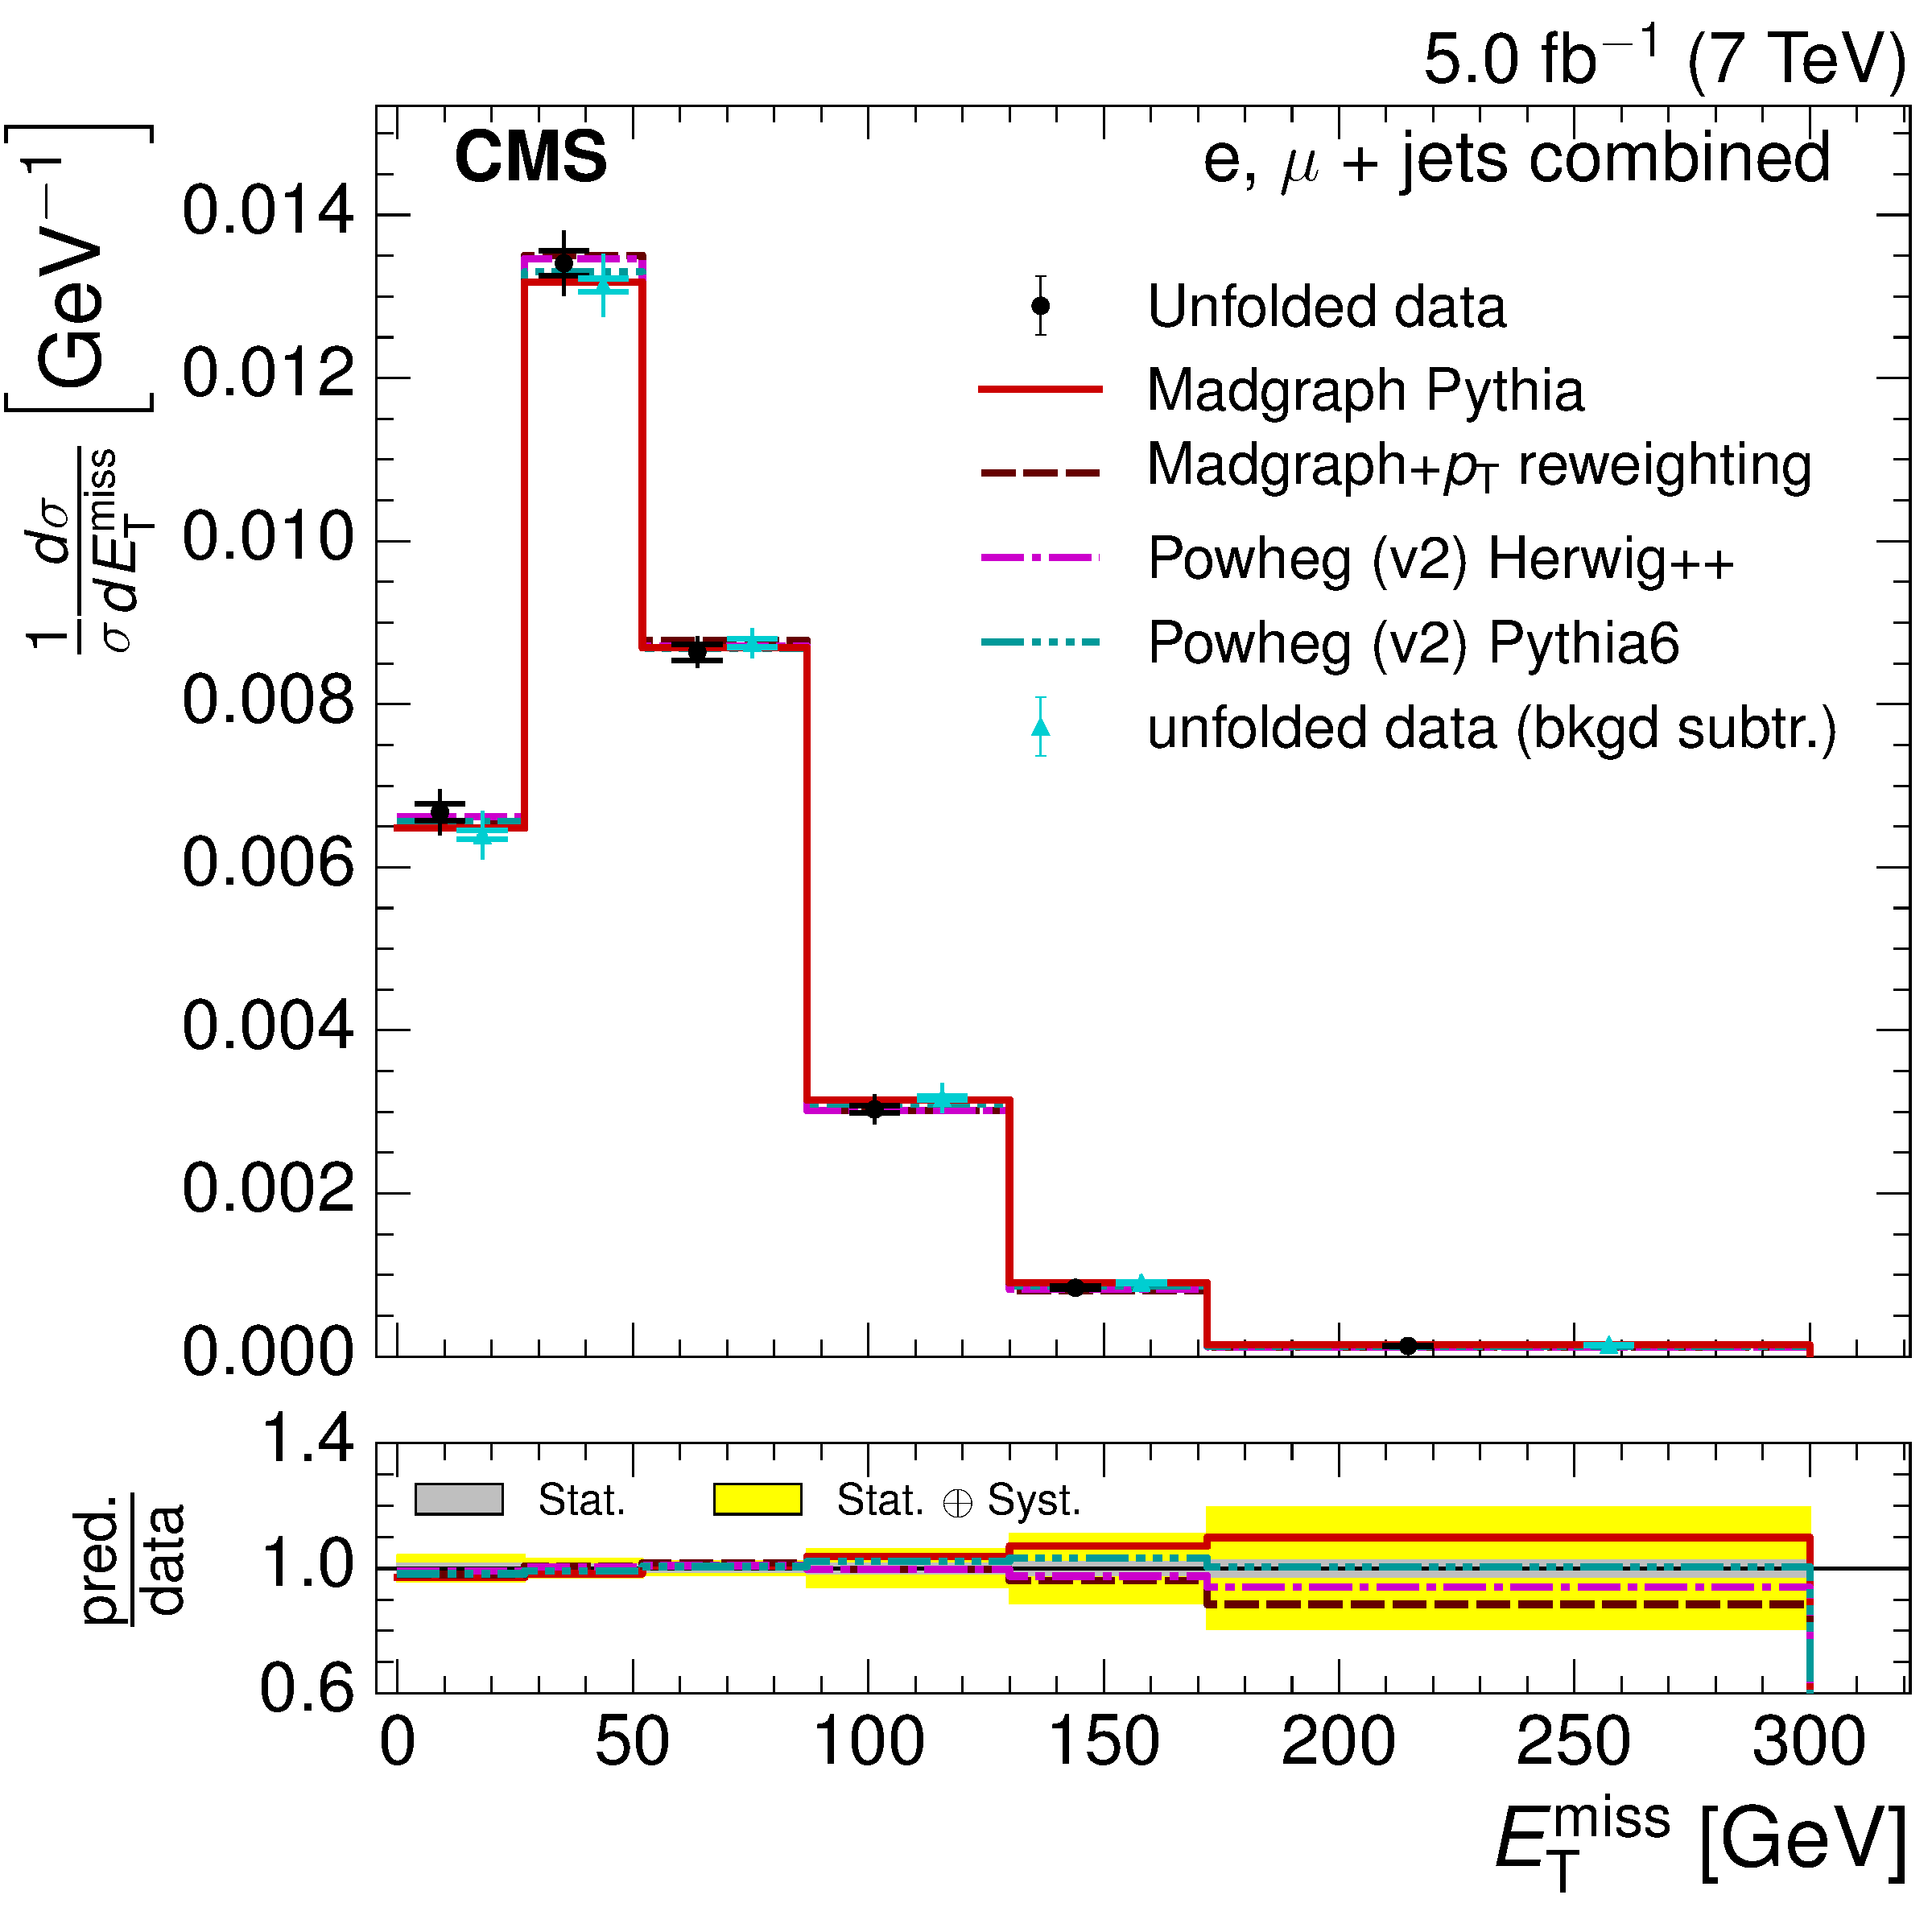
\includegraphics[width=0.32\textwidth]{Chapters/07_08_09_Analysis/Images/results/fit/7TeV/MET/central/normalised_xsection_combined_different_generators_with_bkgd_subtraction_results.pdf}\hfill
     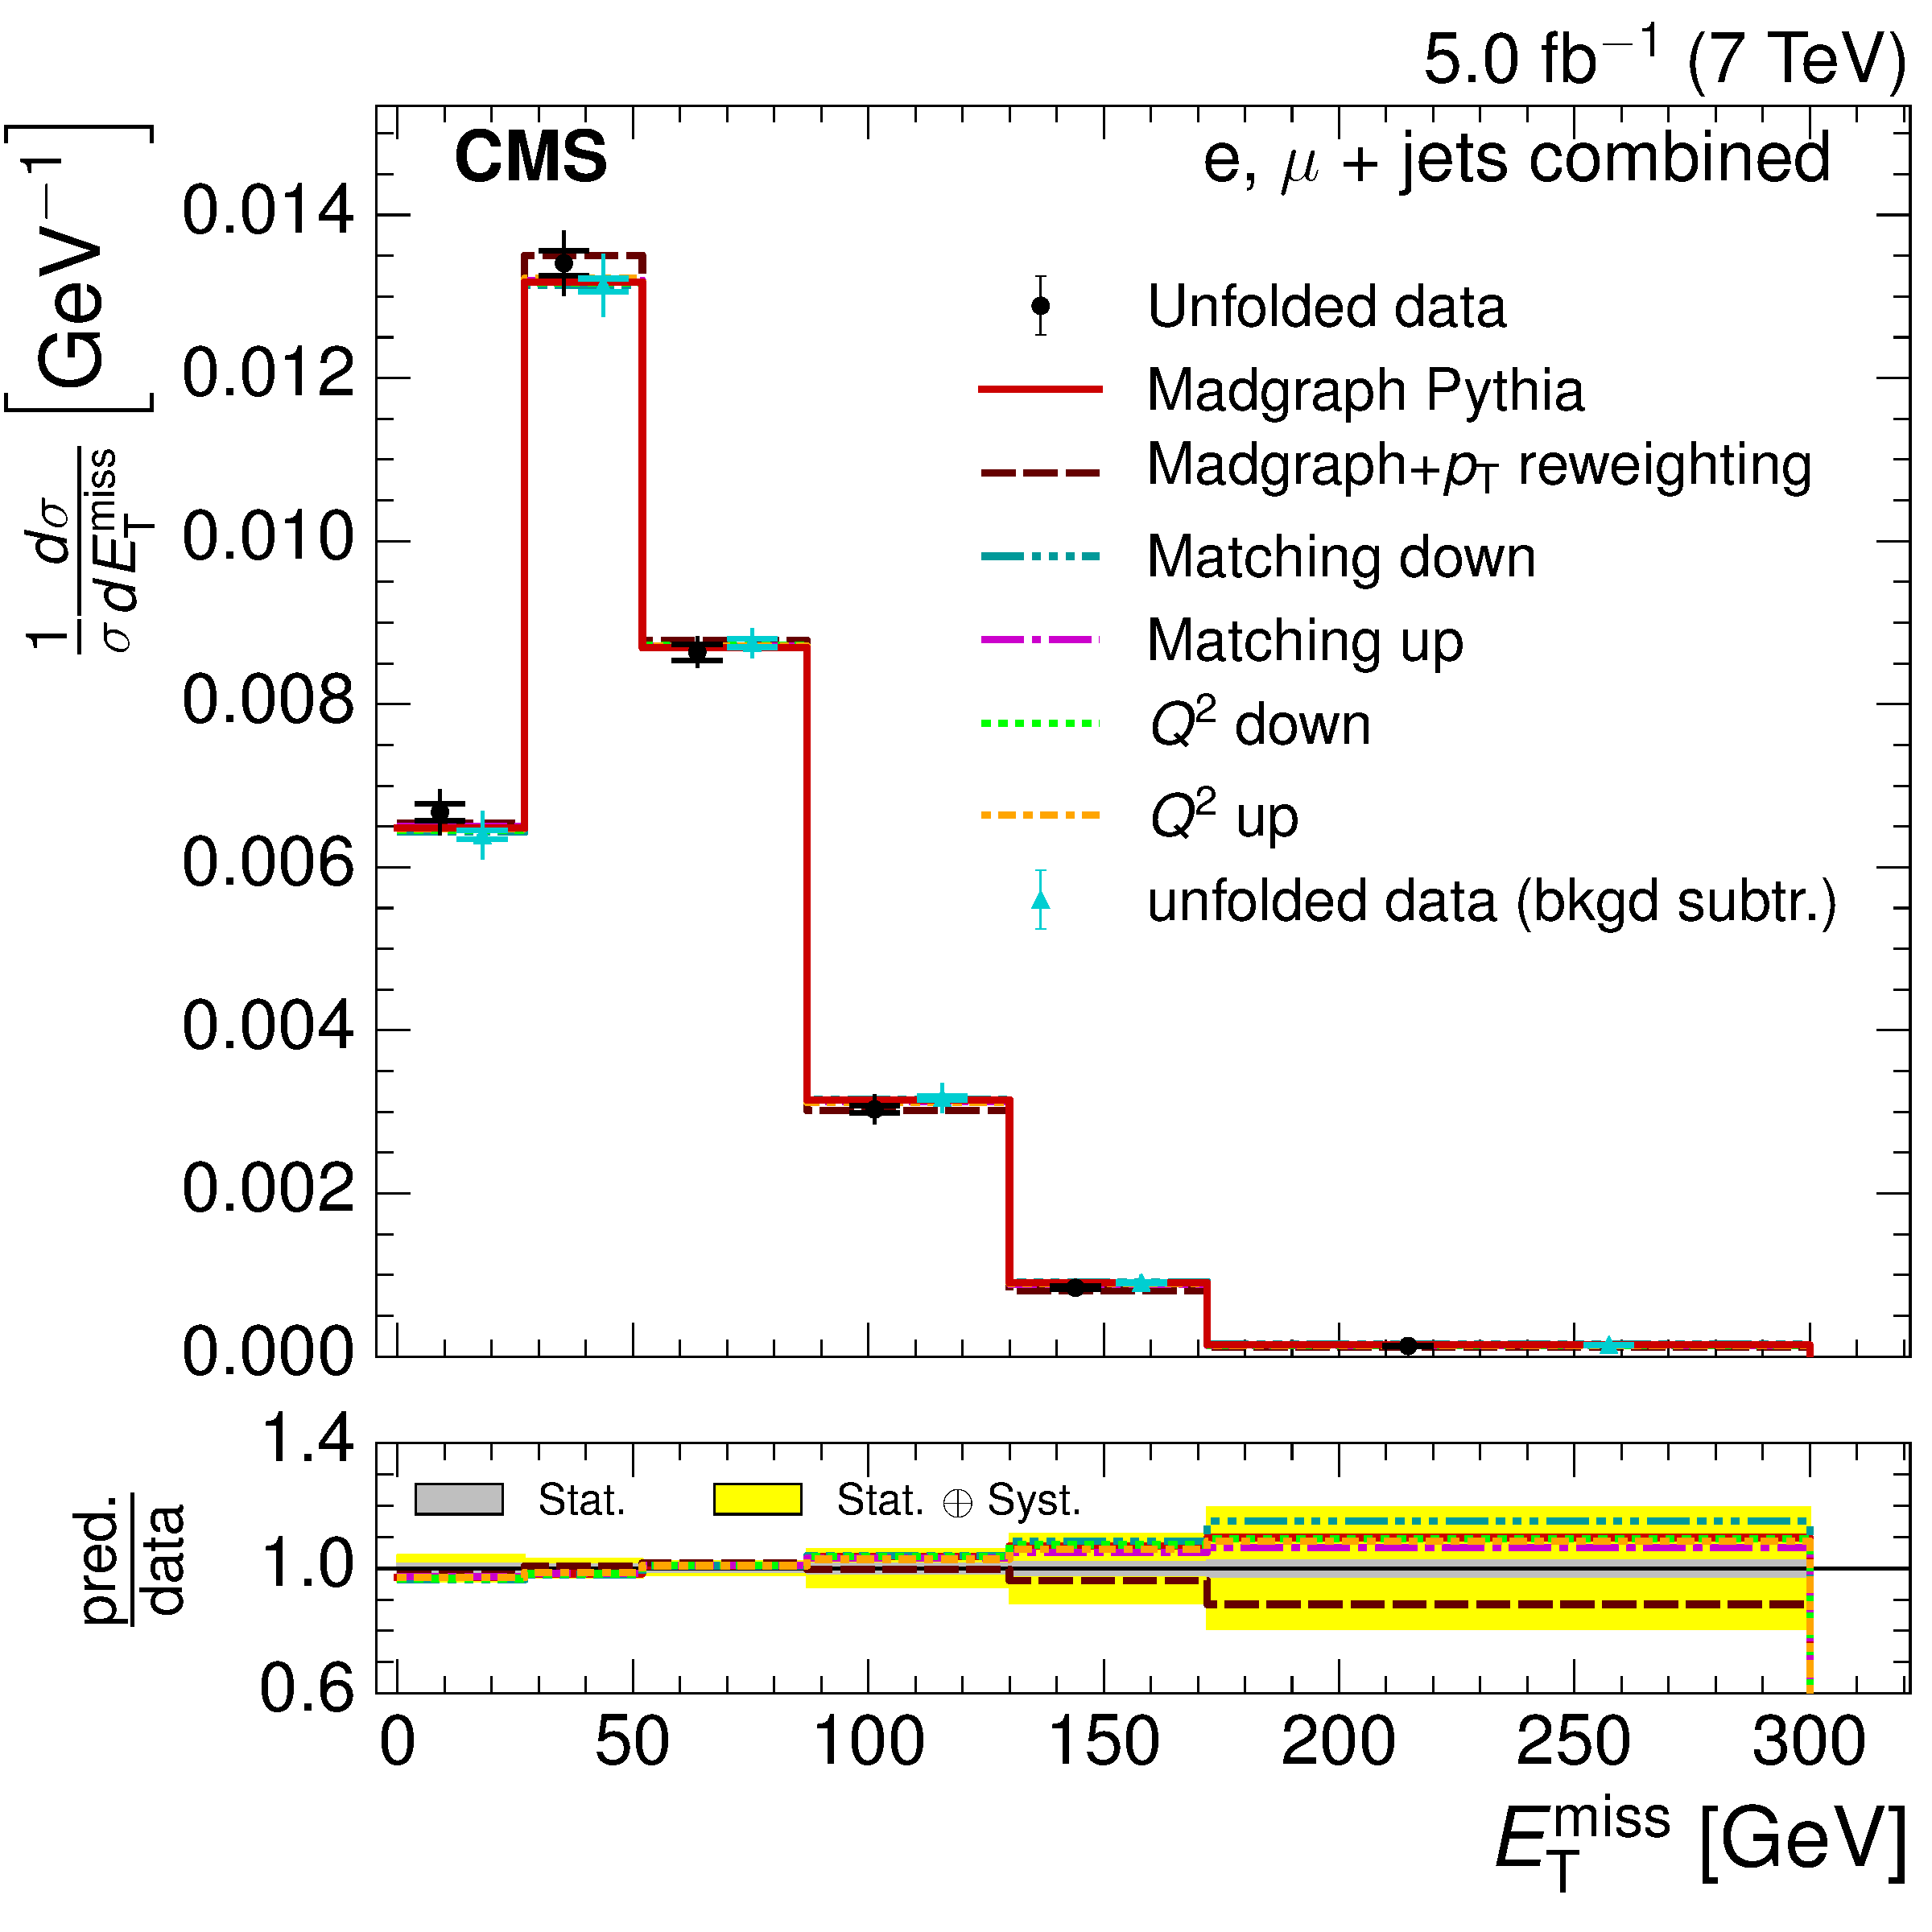
\includegraphics[width=0.32\textwidth]{Chapters/07_08_09_Analysis/Images/results/fit/7TeV/MET/central/normalised_xsection_combined_systematics_shifts_with_bkgd_subtraction_results.pdf}\hfill
     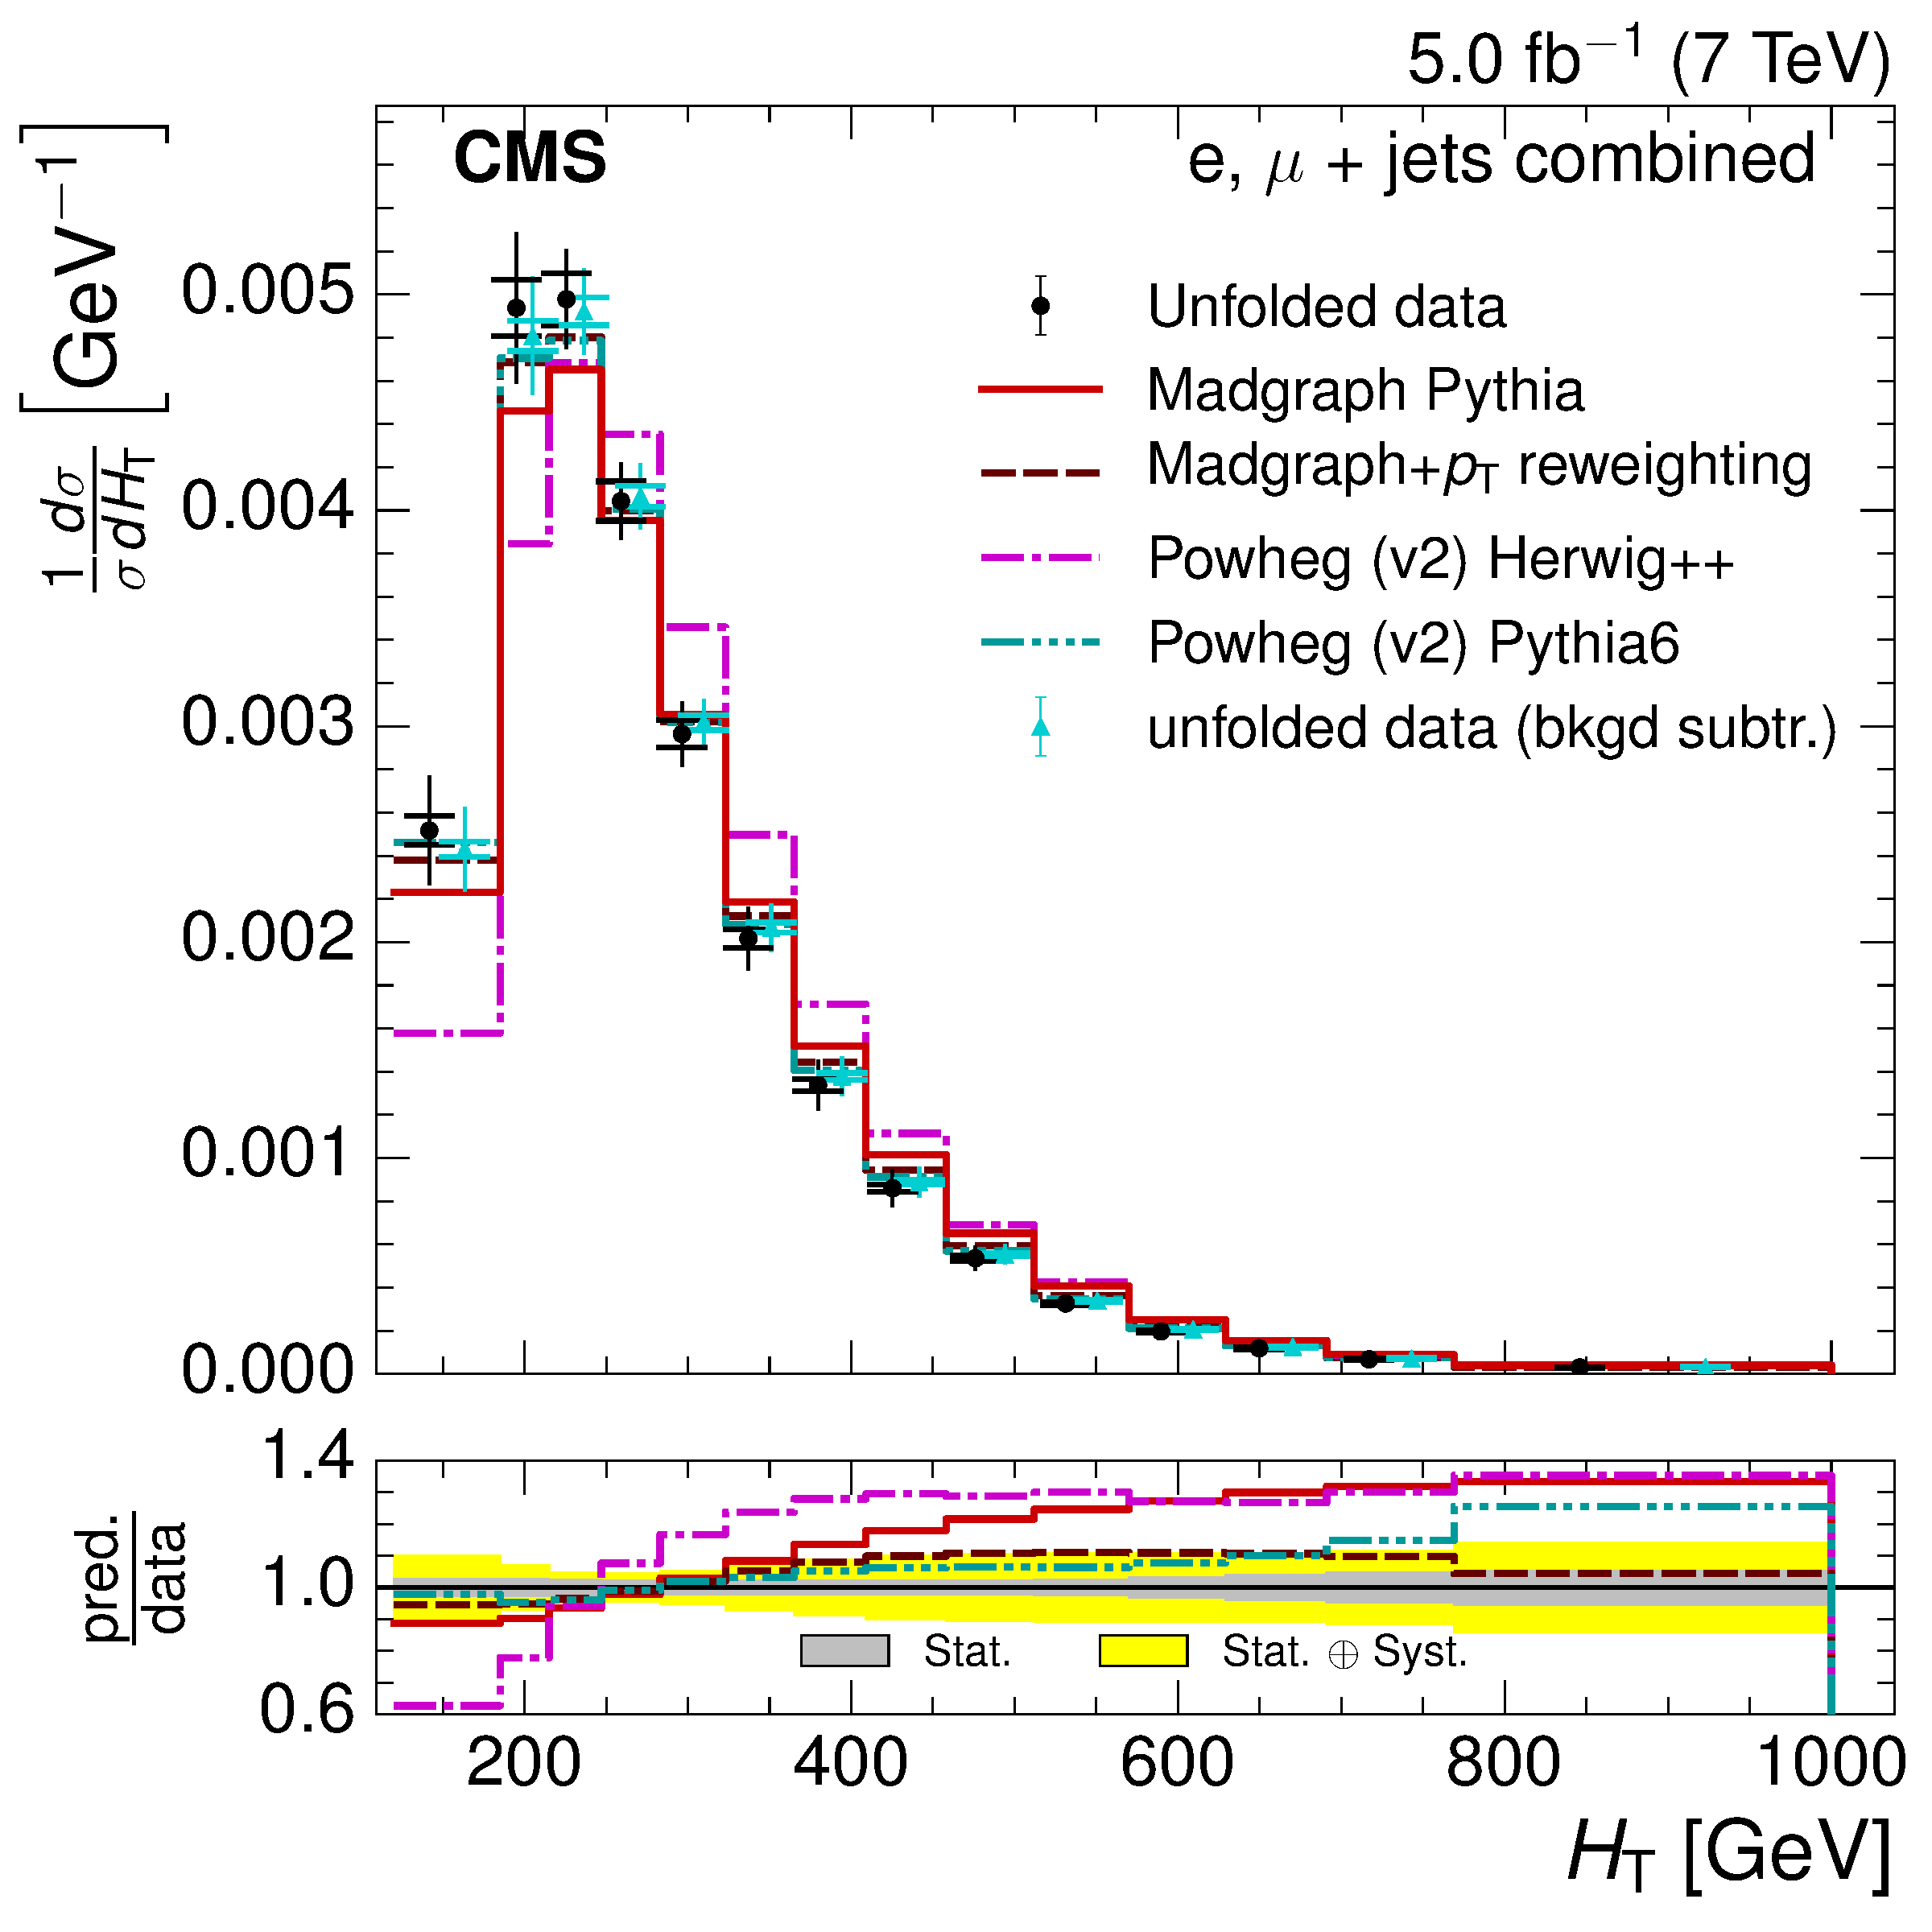
\includegraphics[width=0.32\textwidth]{Chapters/07_08_09_Analysis/Images/results/fit/7TeV/HT/central/normalised_xsection_combined_different_generators_with_bkgd_subtraction_results.pdf}\\
     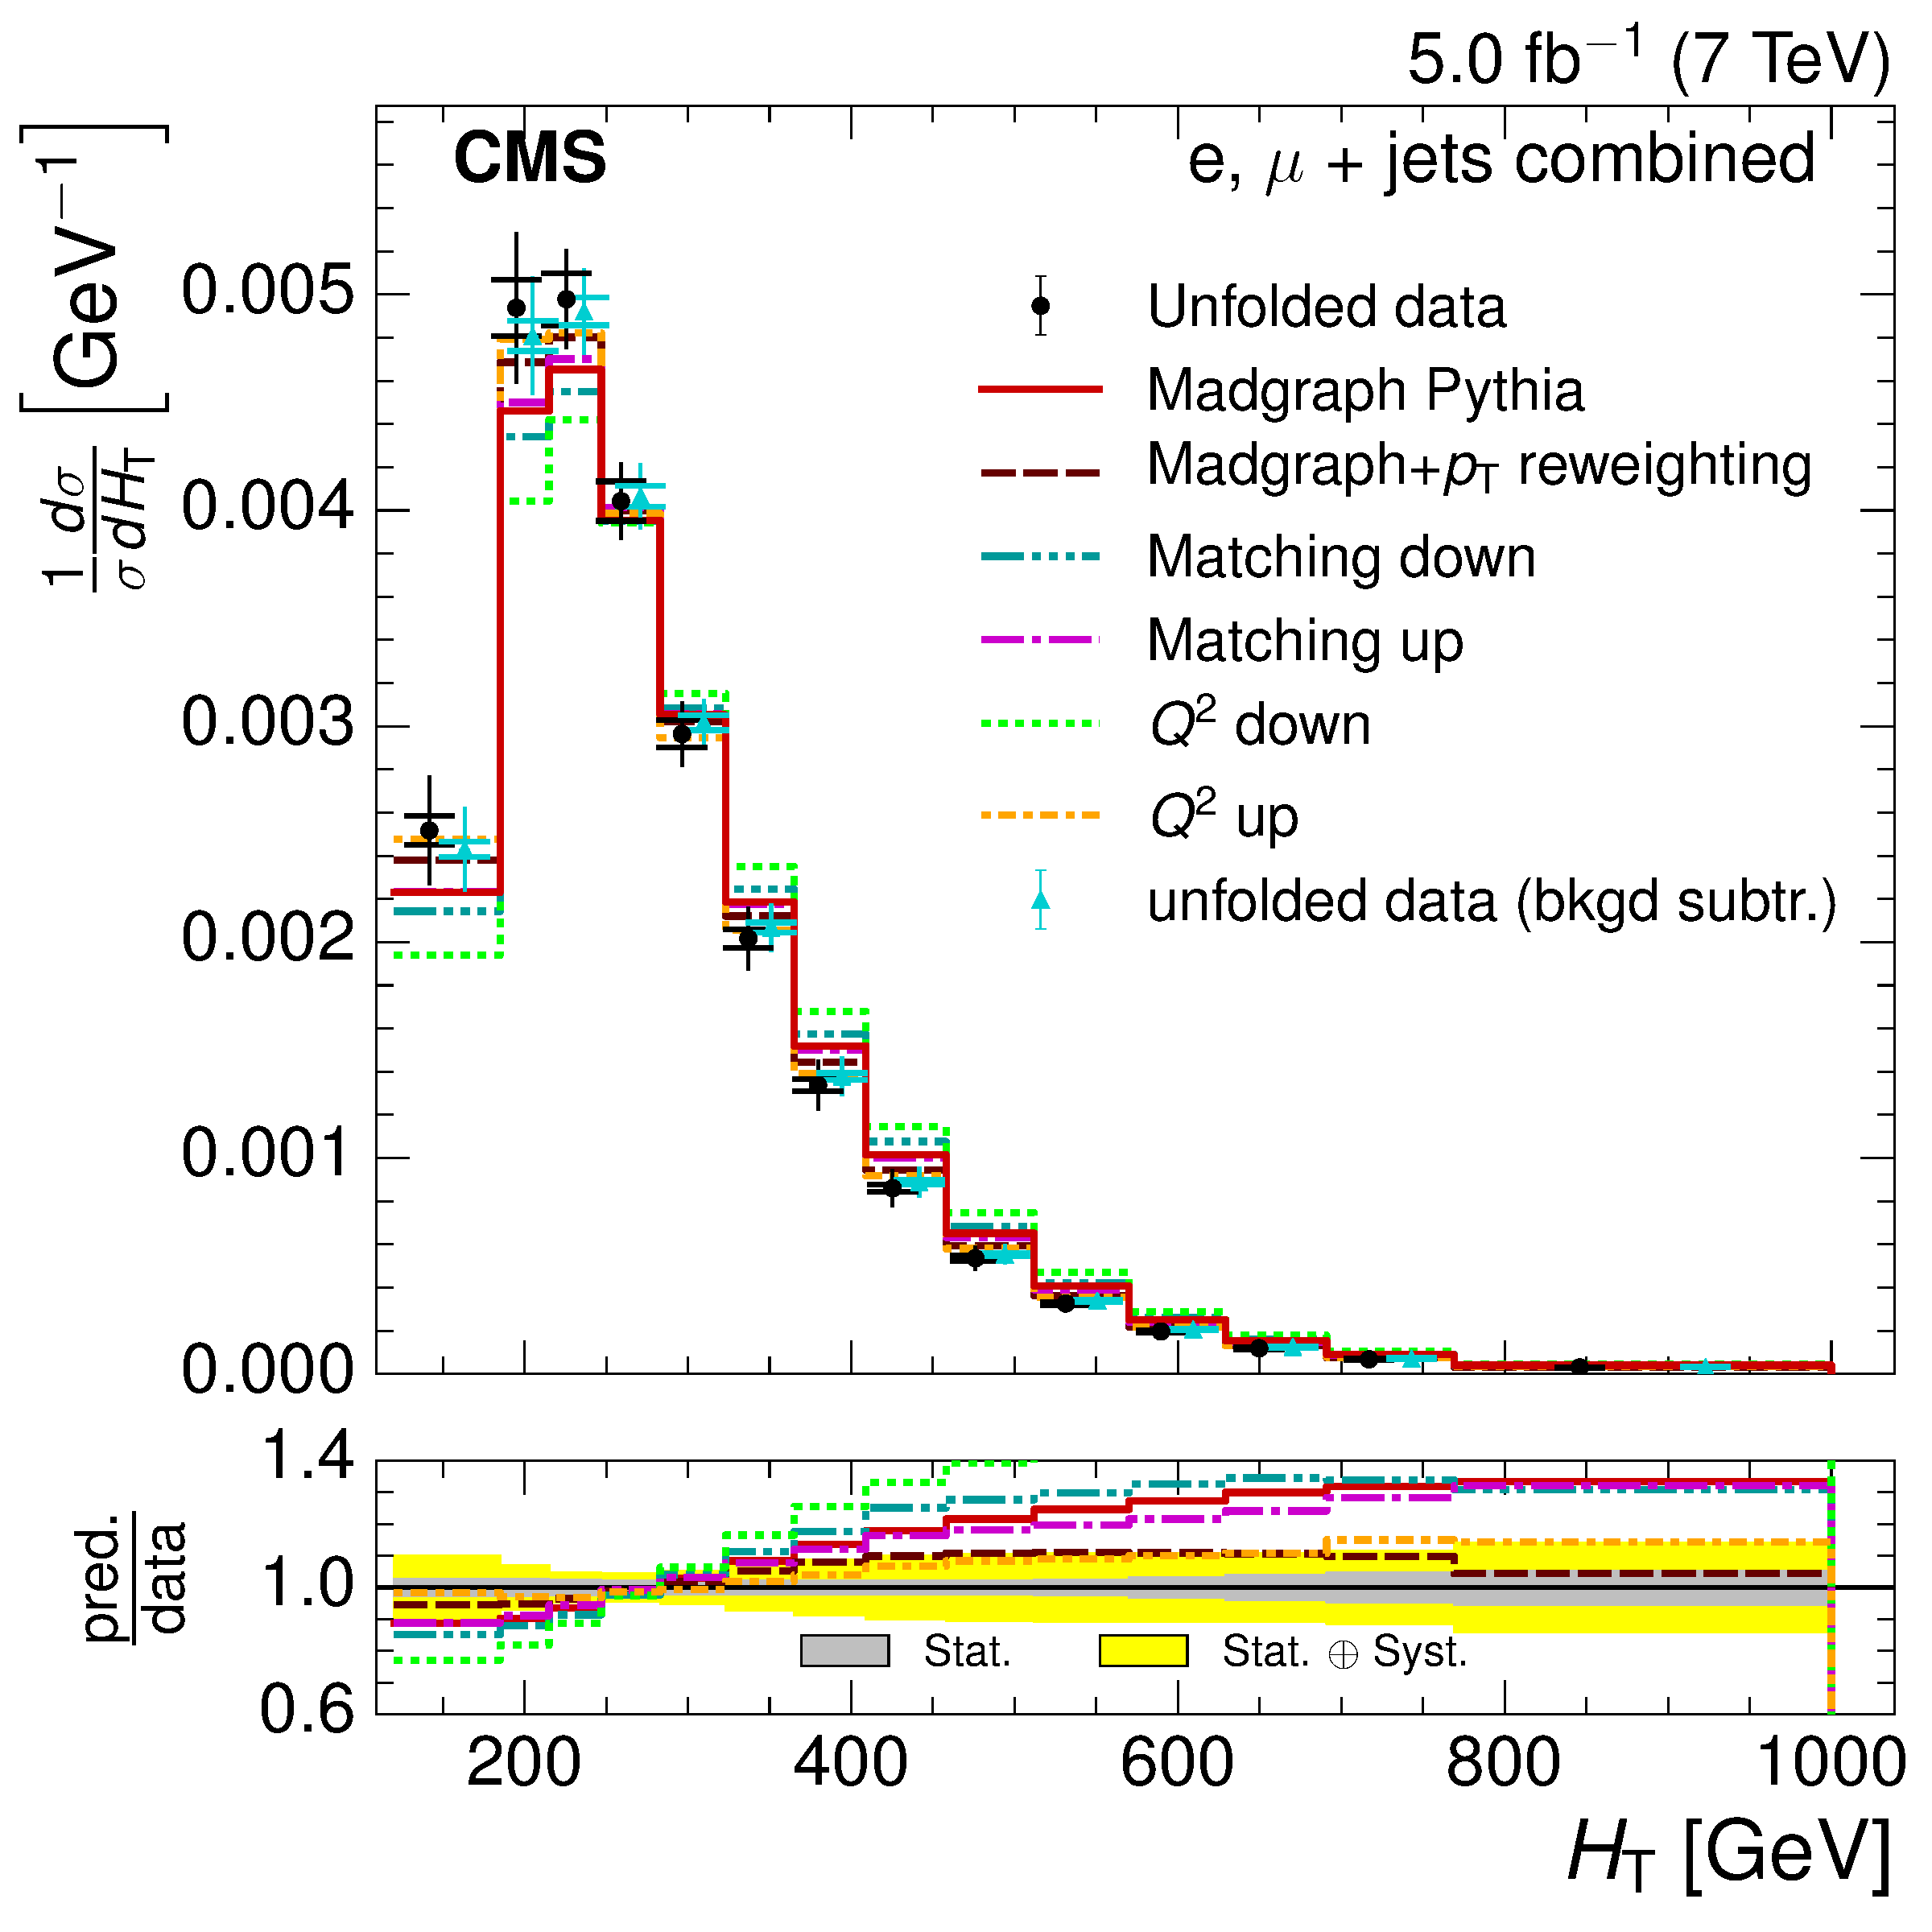
\includegraphics[width=0.32\textwidth]{Chapters/07_08_09_Analysis/Images/results/fit/7TeV/HT/central/normalised_xsection_combined_systematics_shifts_with_bkgd_subtraction_results.pdf}\hfill
     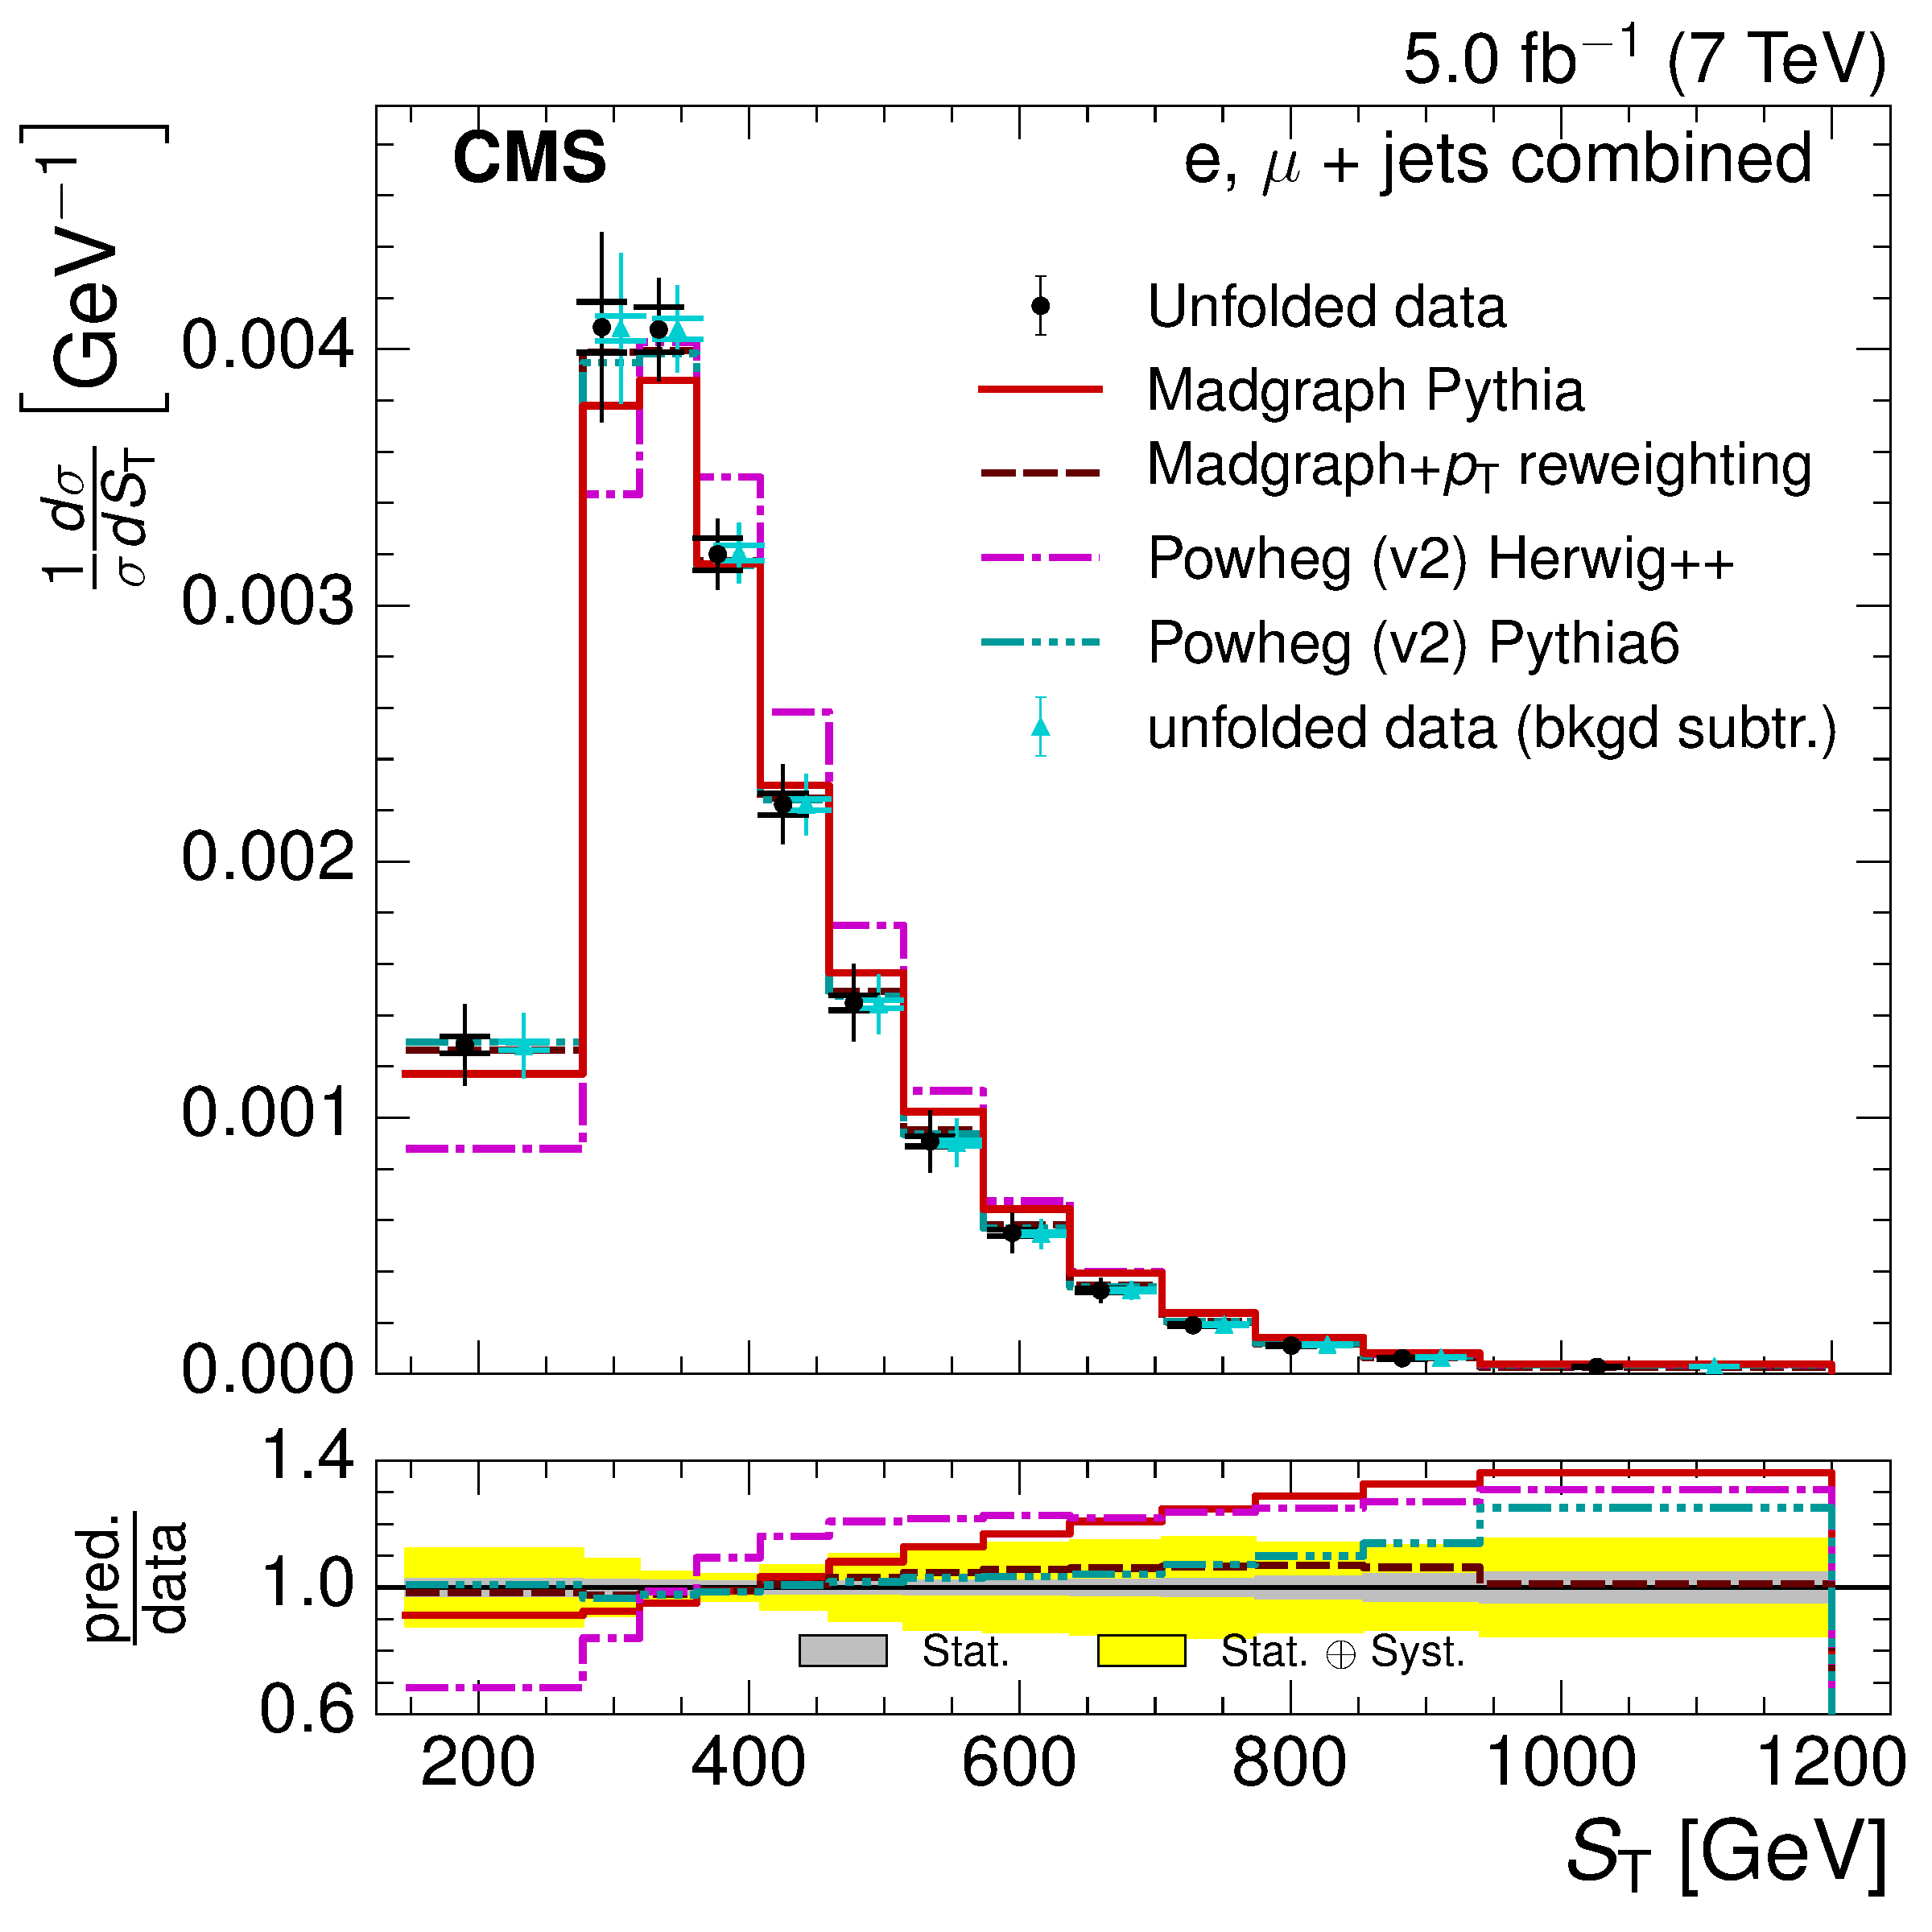
\includegraphics[width=0.32\textwidth]{Chapters/07_08_09_Analysis/Images/results/fit/7TeV/ST/central/normalised_xsection_combined_different_generators_with_bkgd_subtraction_results.pdf}\hfill
     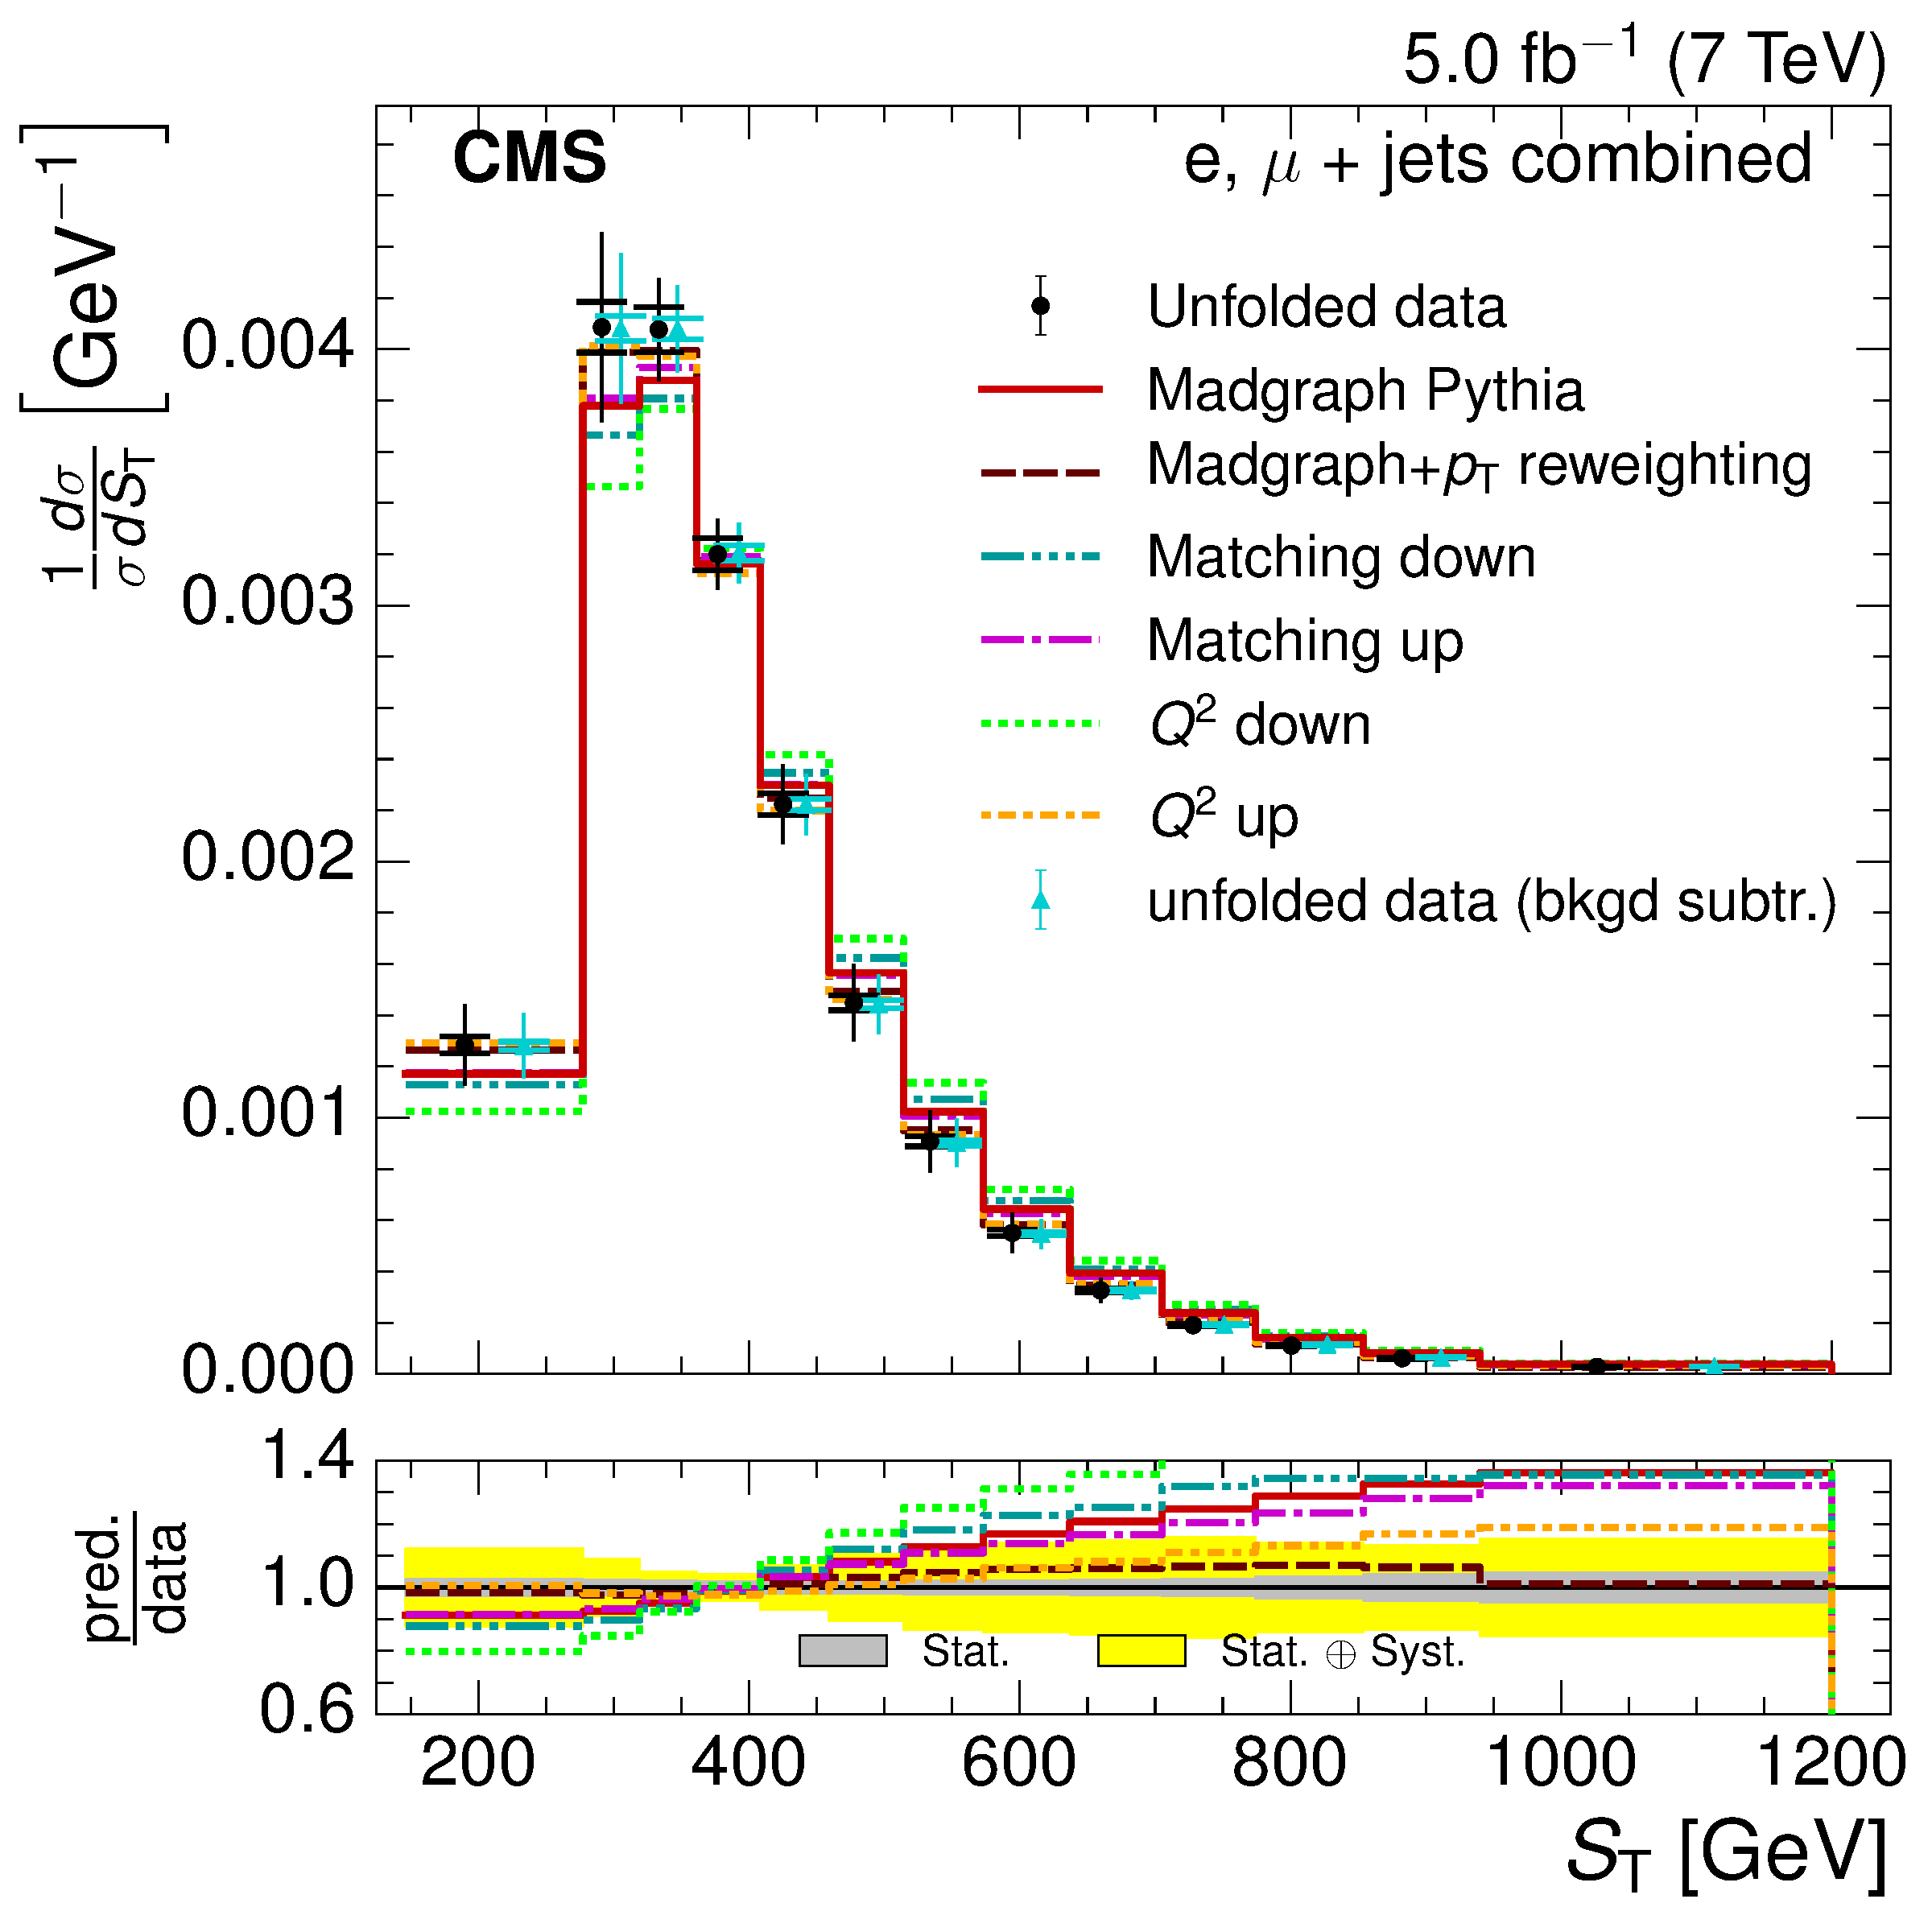
\includegraphics[width=0.32\textwidth]{Chapters/07_08_09_Analysis/Images/results/fit/7TeV/ST/central/normalised_xsection_combined_systematics_shifts_with_bkgd_subtraction_results.pdf}\\
     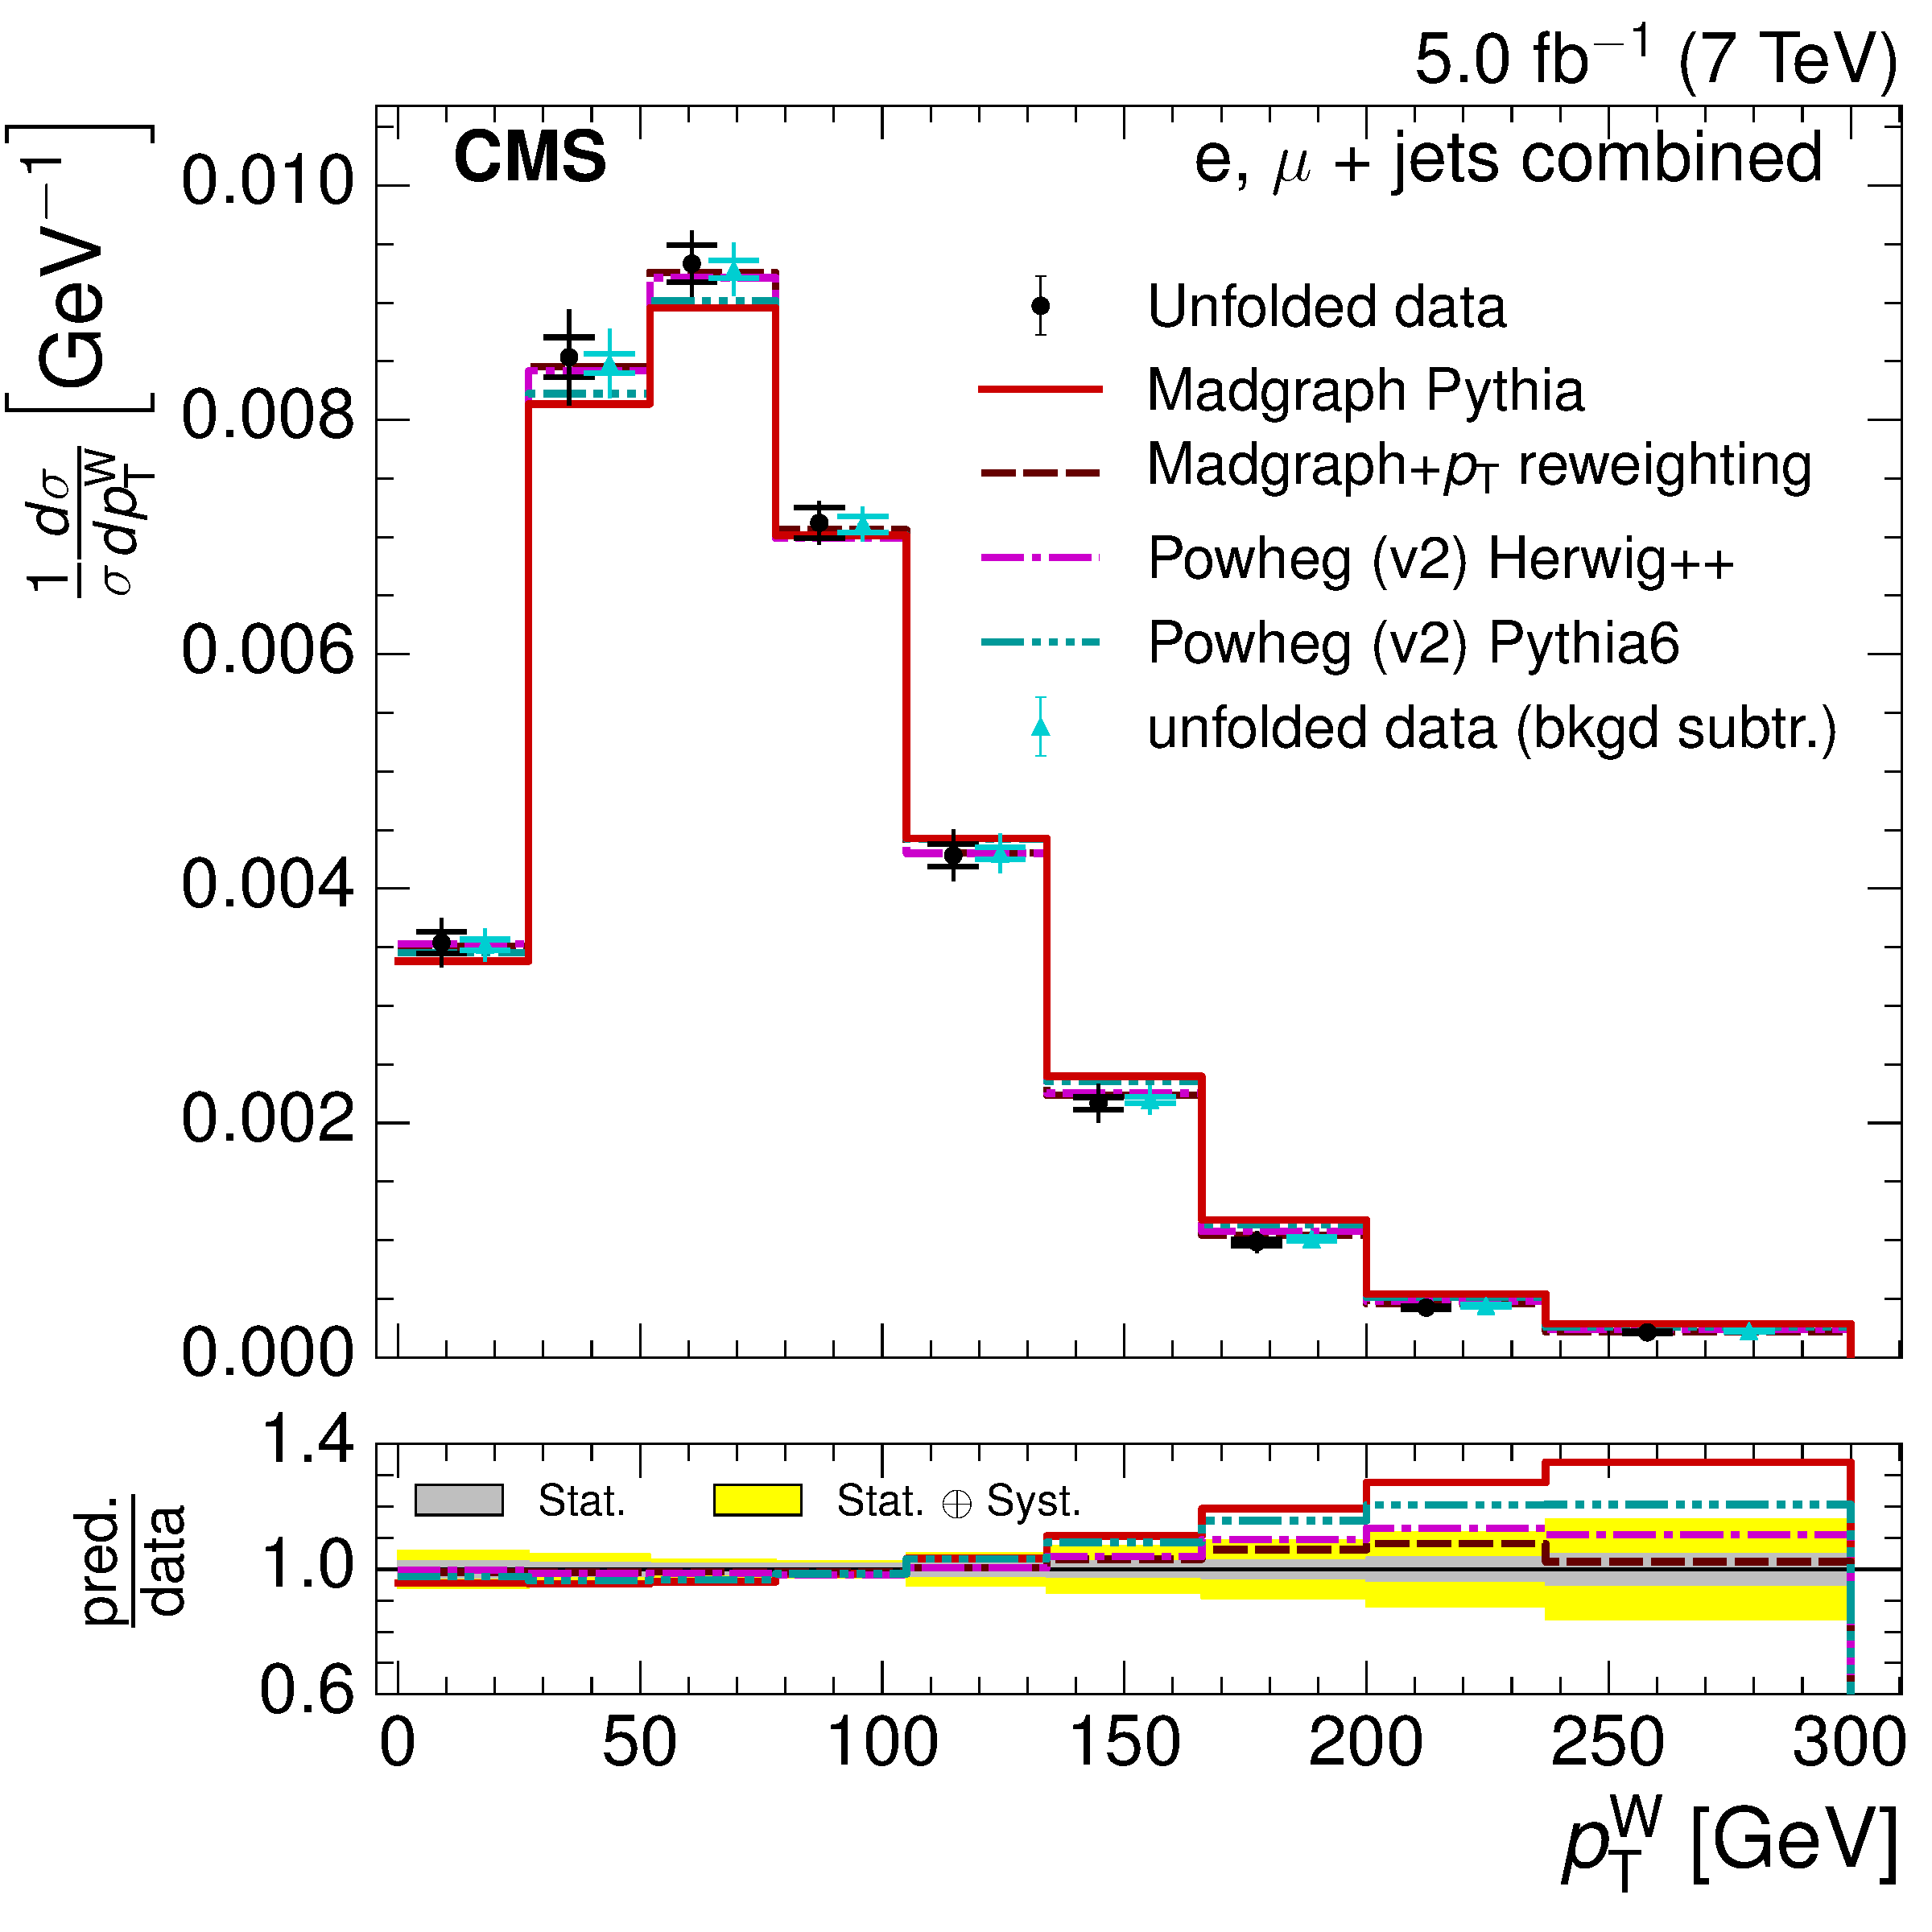
\includegraphics[width=0.32\textwidth]{Chapters/07_08_09_Analysis/Images/results/fit/7TeV/WPT/central/normalised_xsection_combined_different_generators_with_bkgd_subtraction_results.pdf}\hfill
     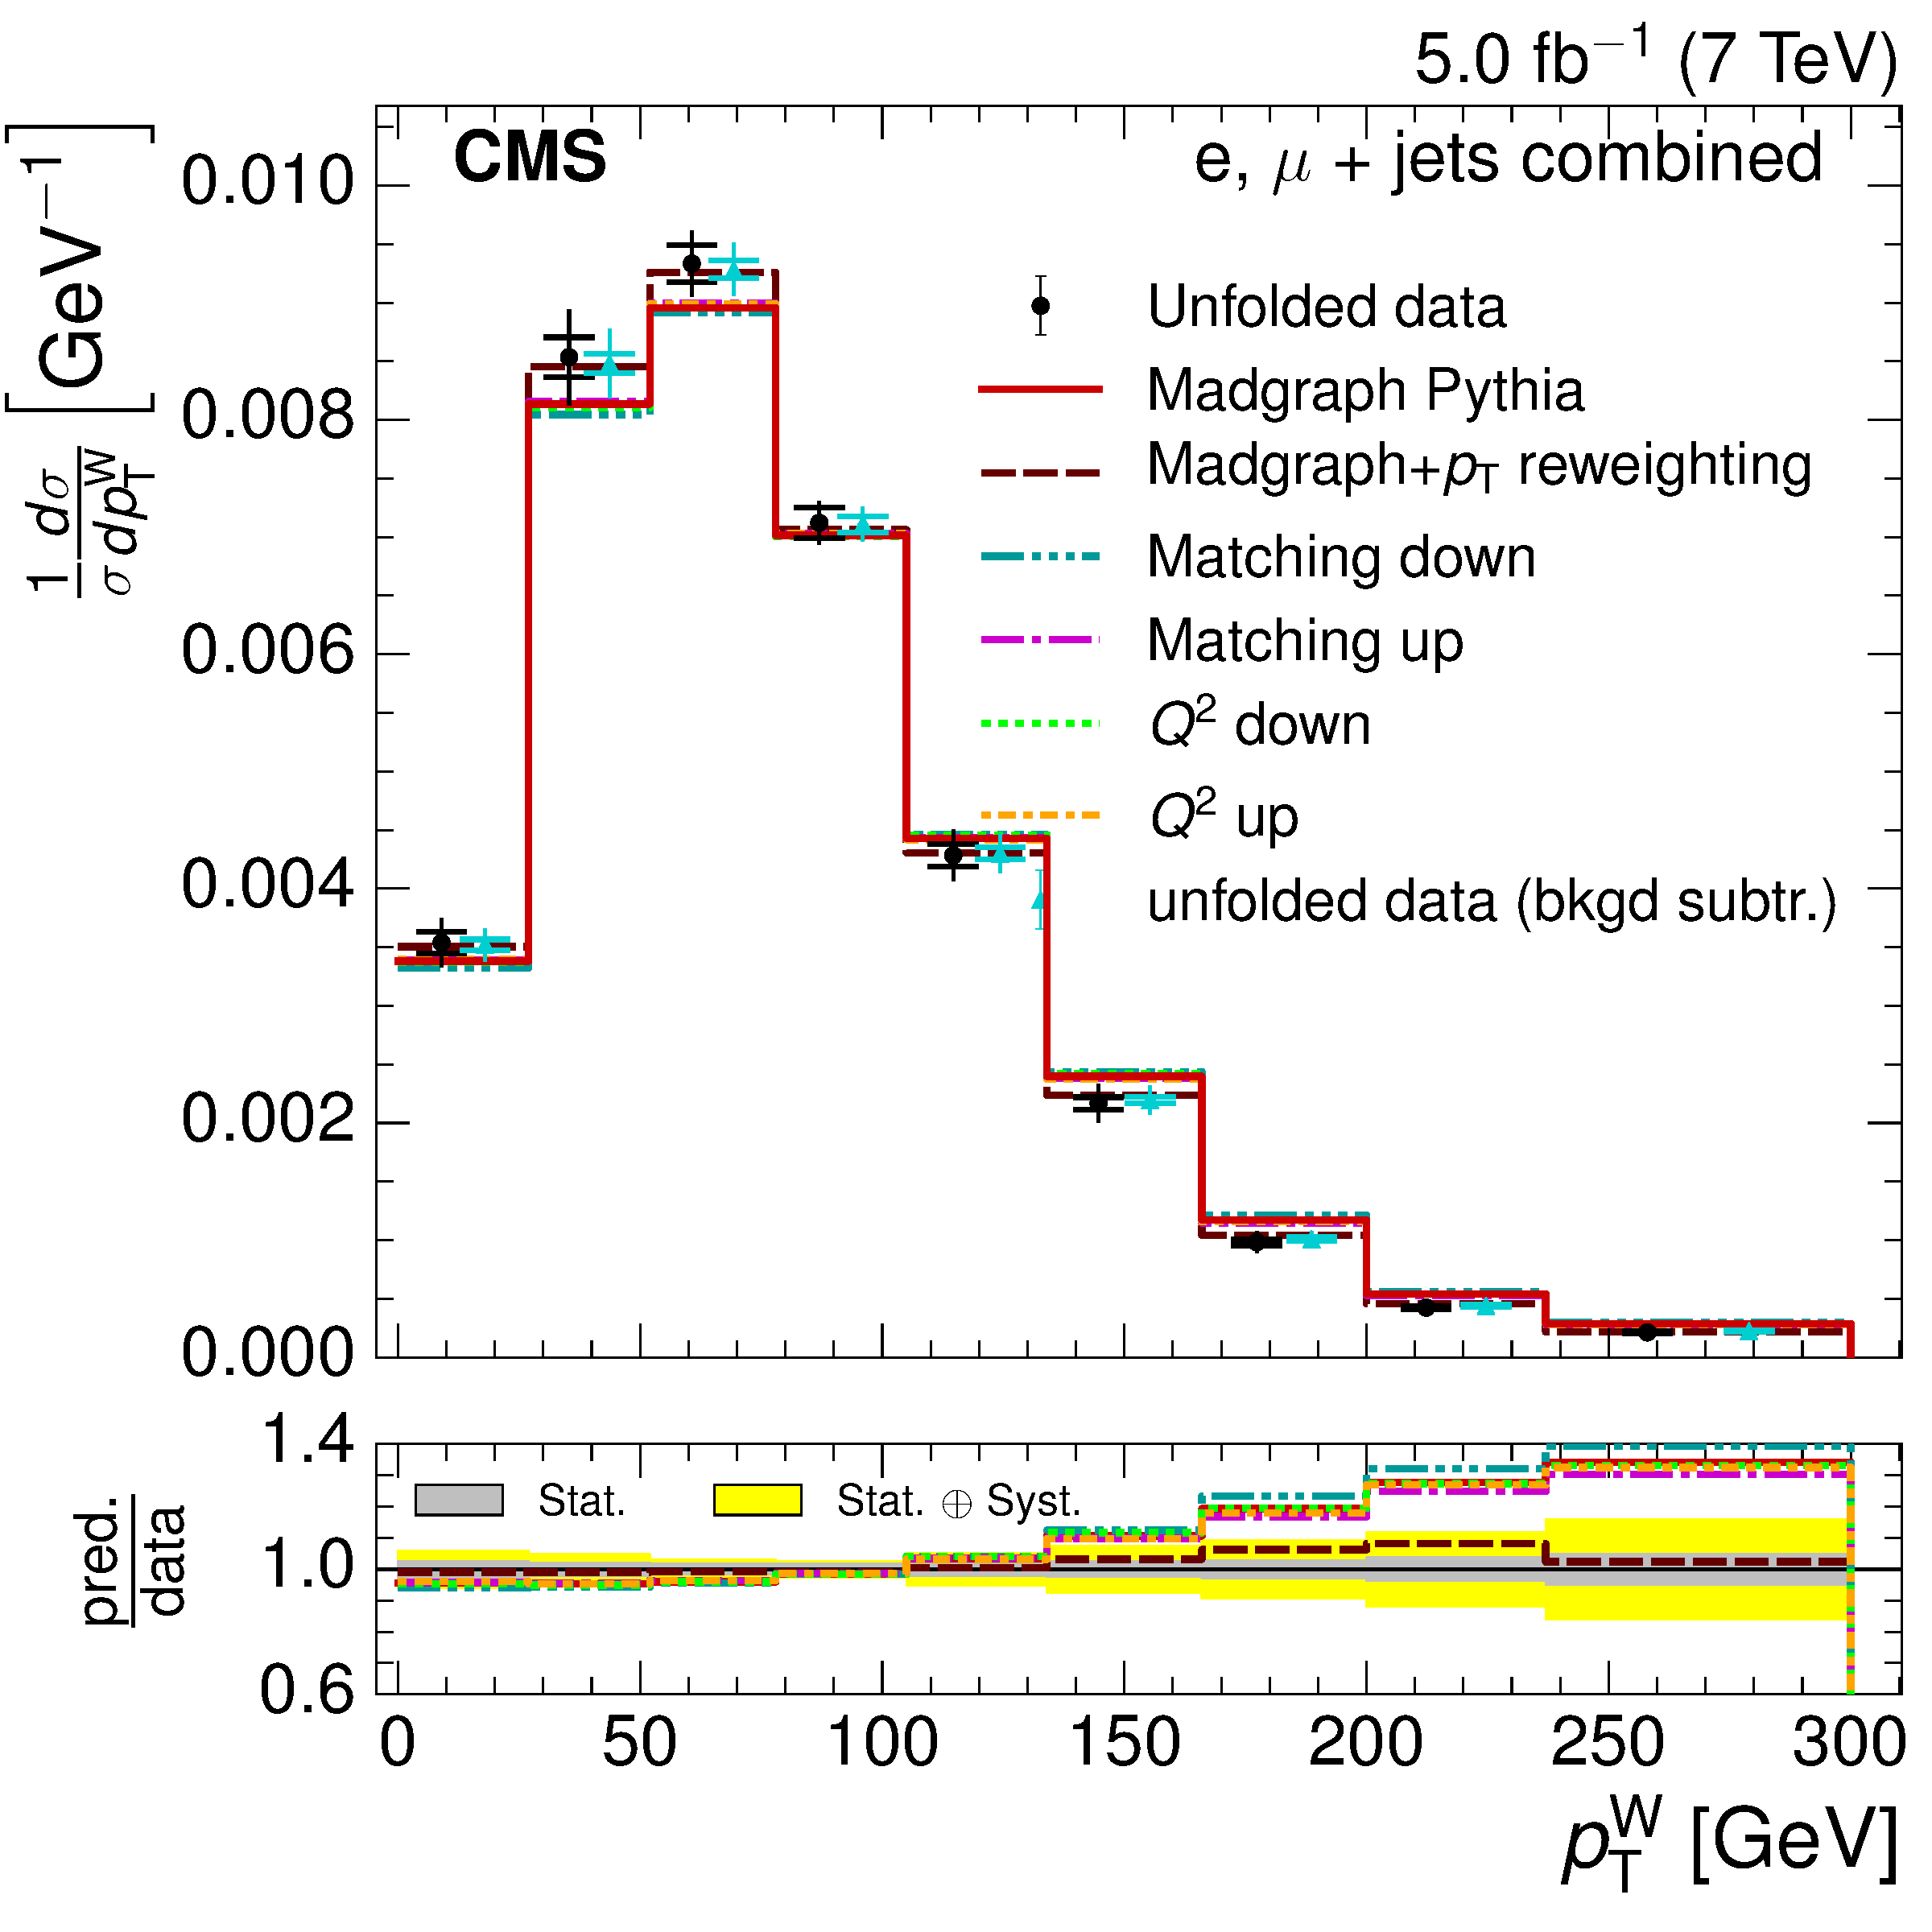
\includegraphics[width=0.32\textwidth]{Chapters/07_08_09_Analysis/Images/results/fit/7TeV/WPT/central/normalised_xsection_combined_systematics_shifts_with_bkgd_subtraction_results.pdf}\hfill
     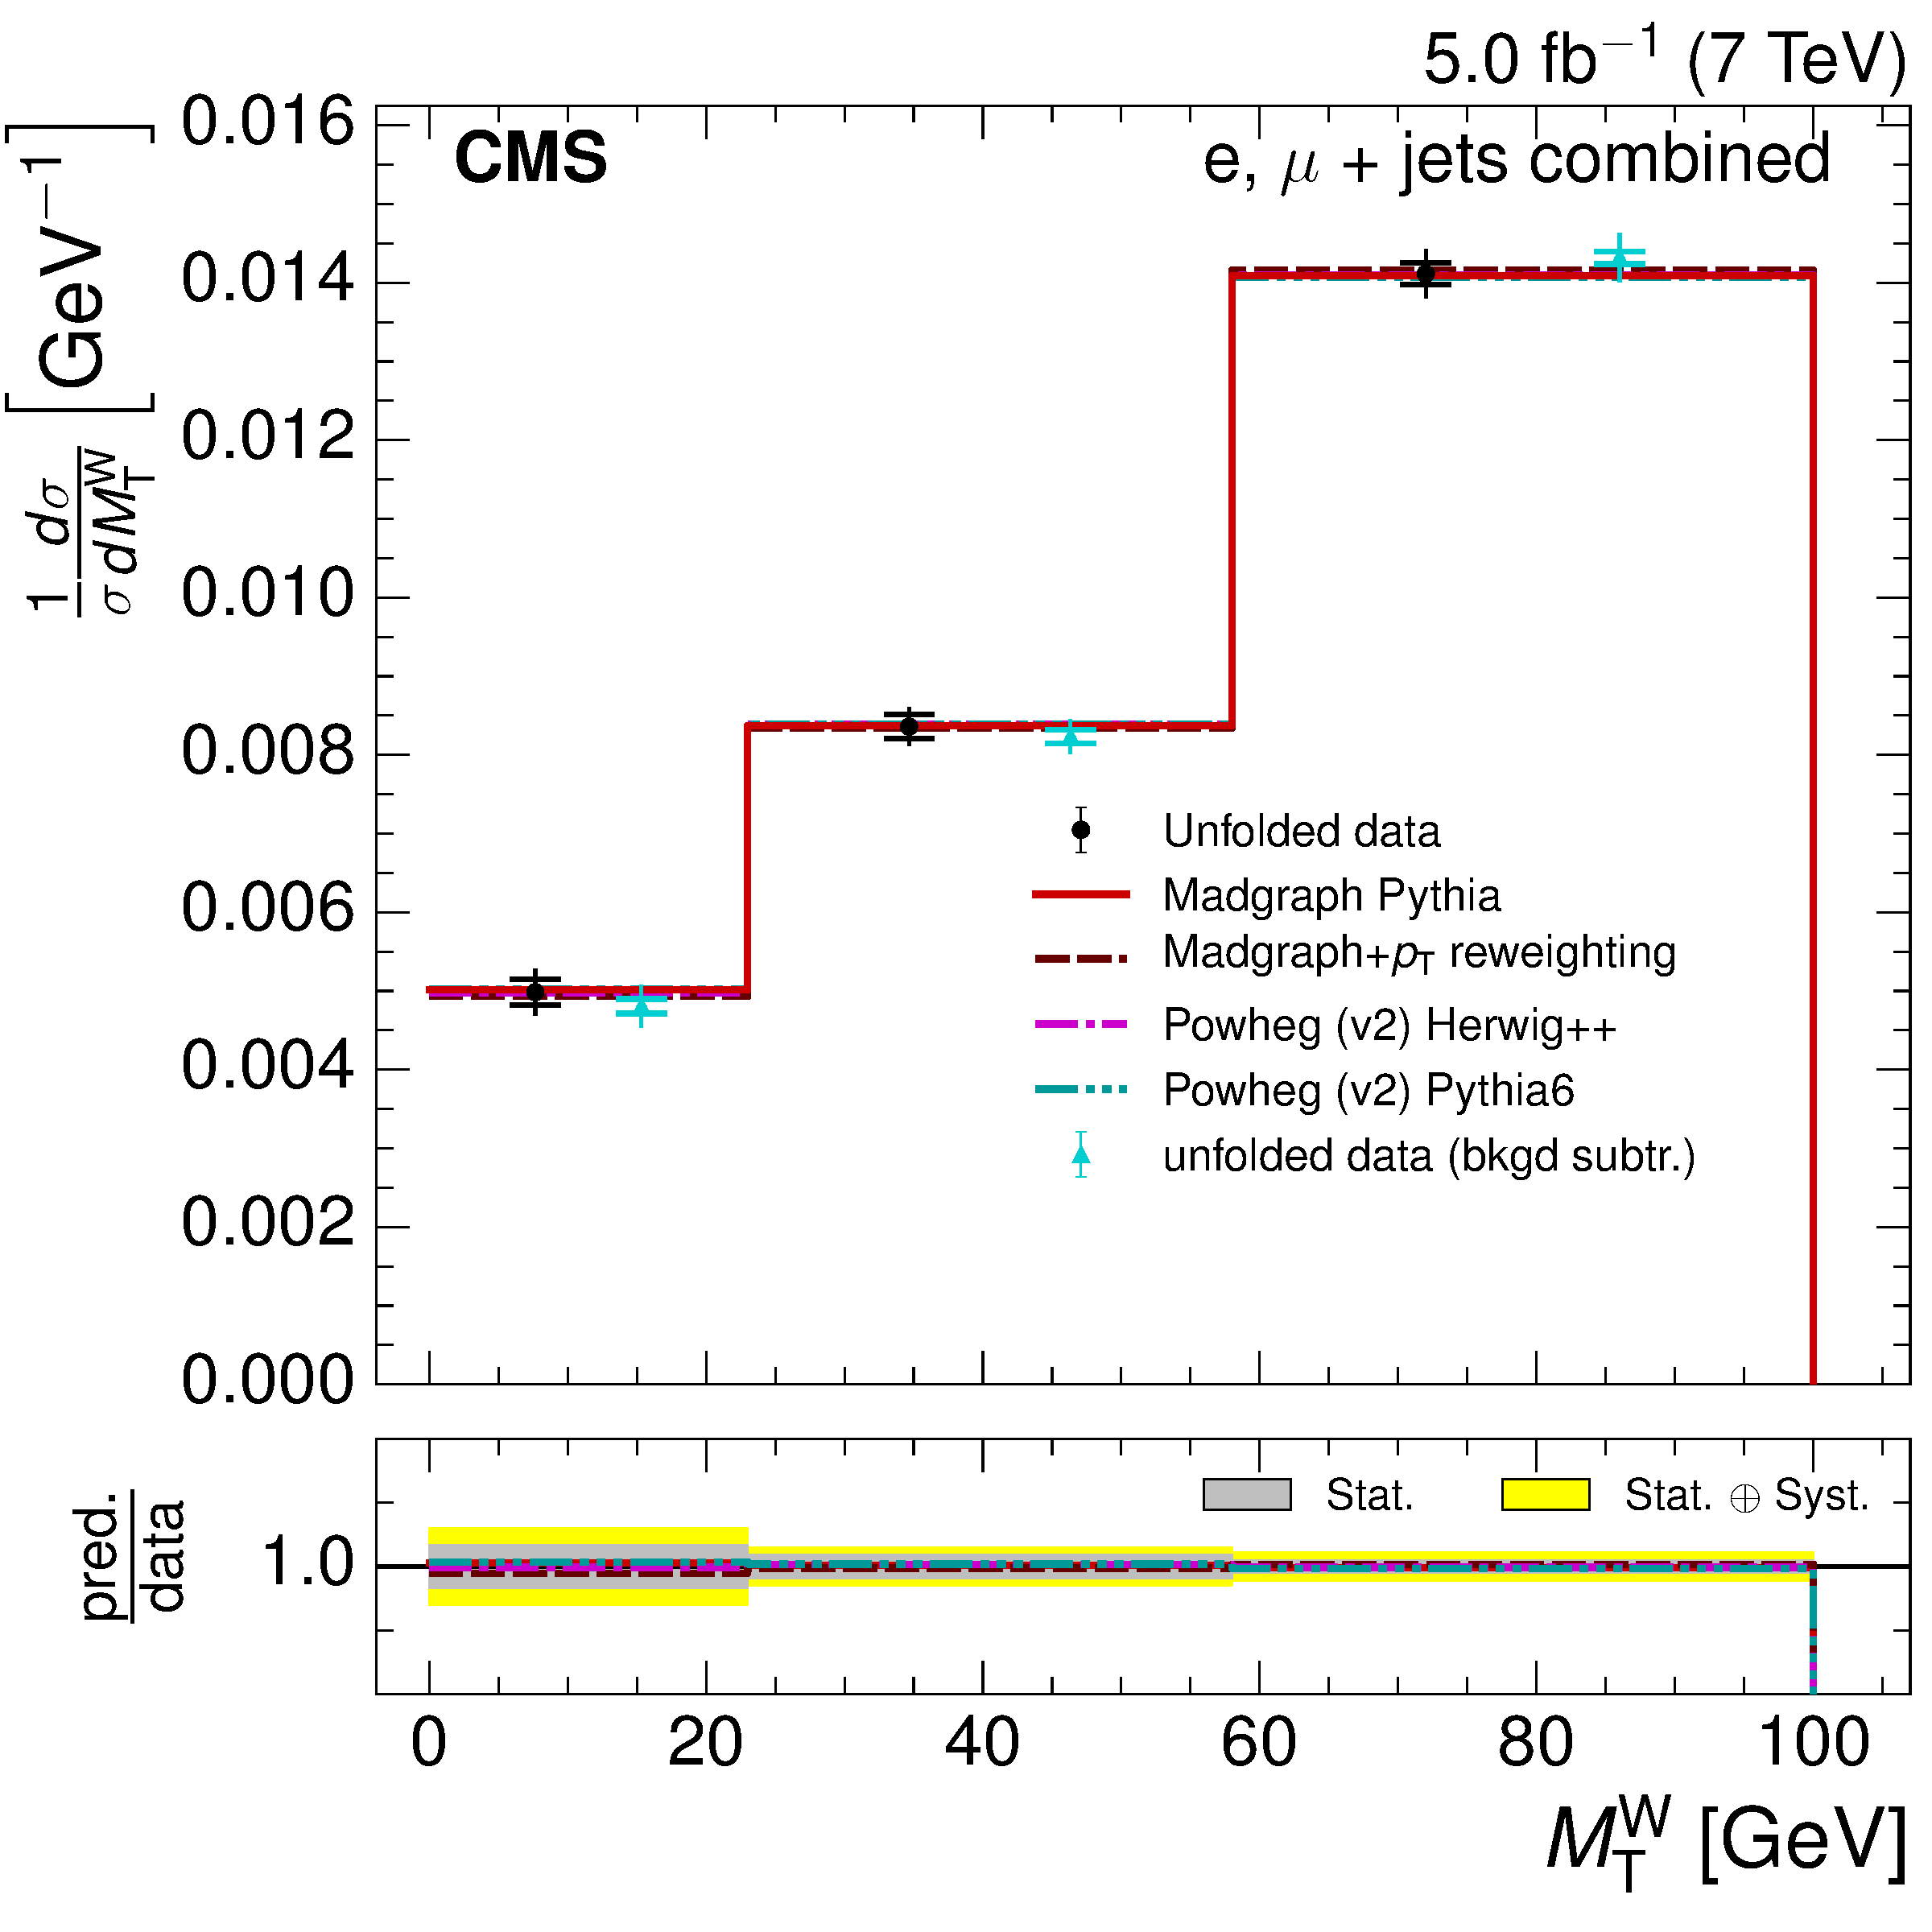
\includegraphics[width=0.32\textwidth]{Chapters/07_08_09_Analysis/Images/results/fit/7TeV/MT/central/normalised_xsection_combined_different_generators_with_bkgd_subtraction_results.pdf}\\
     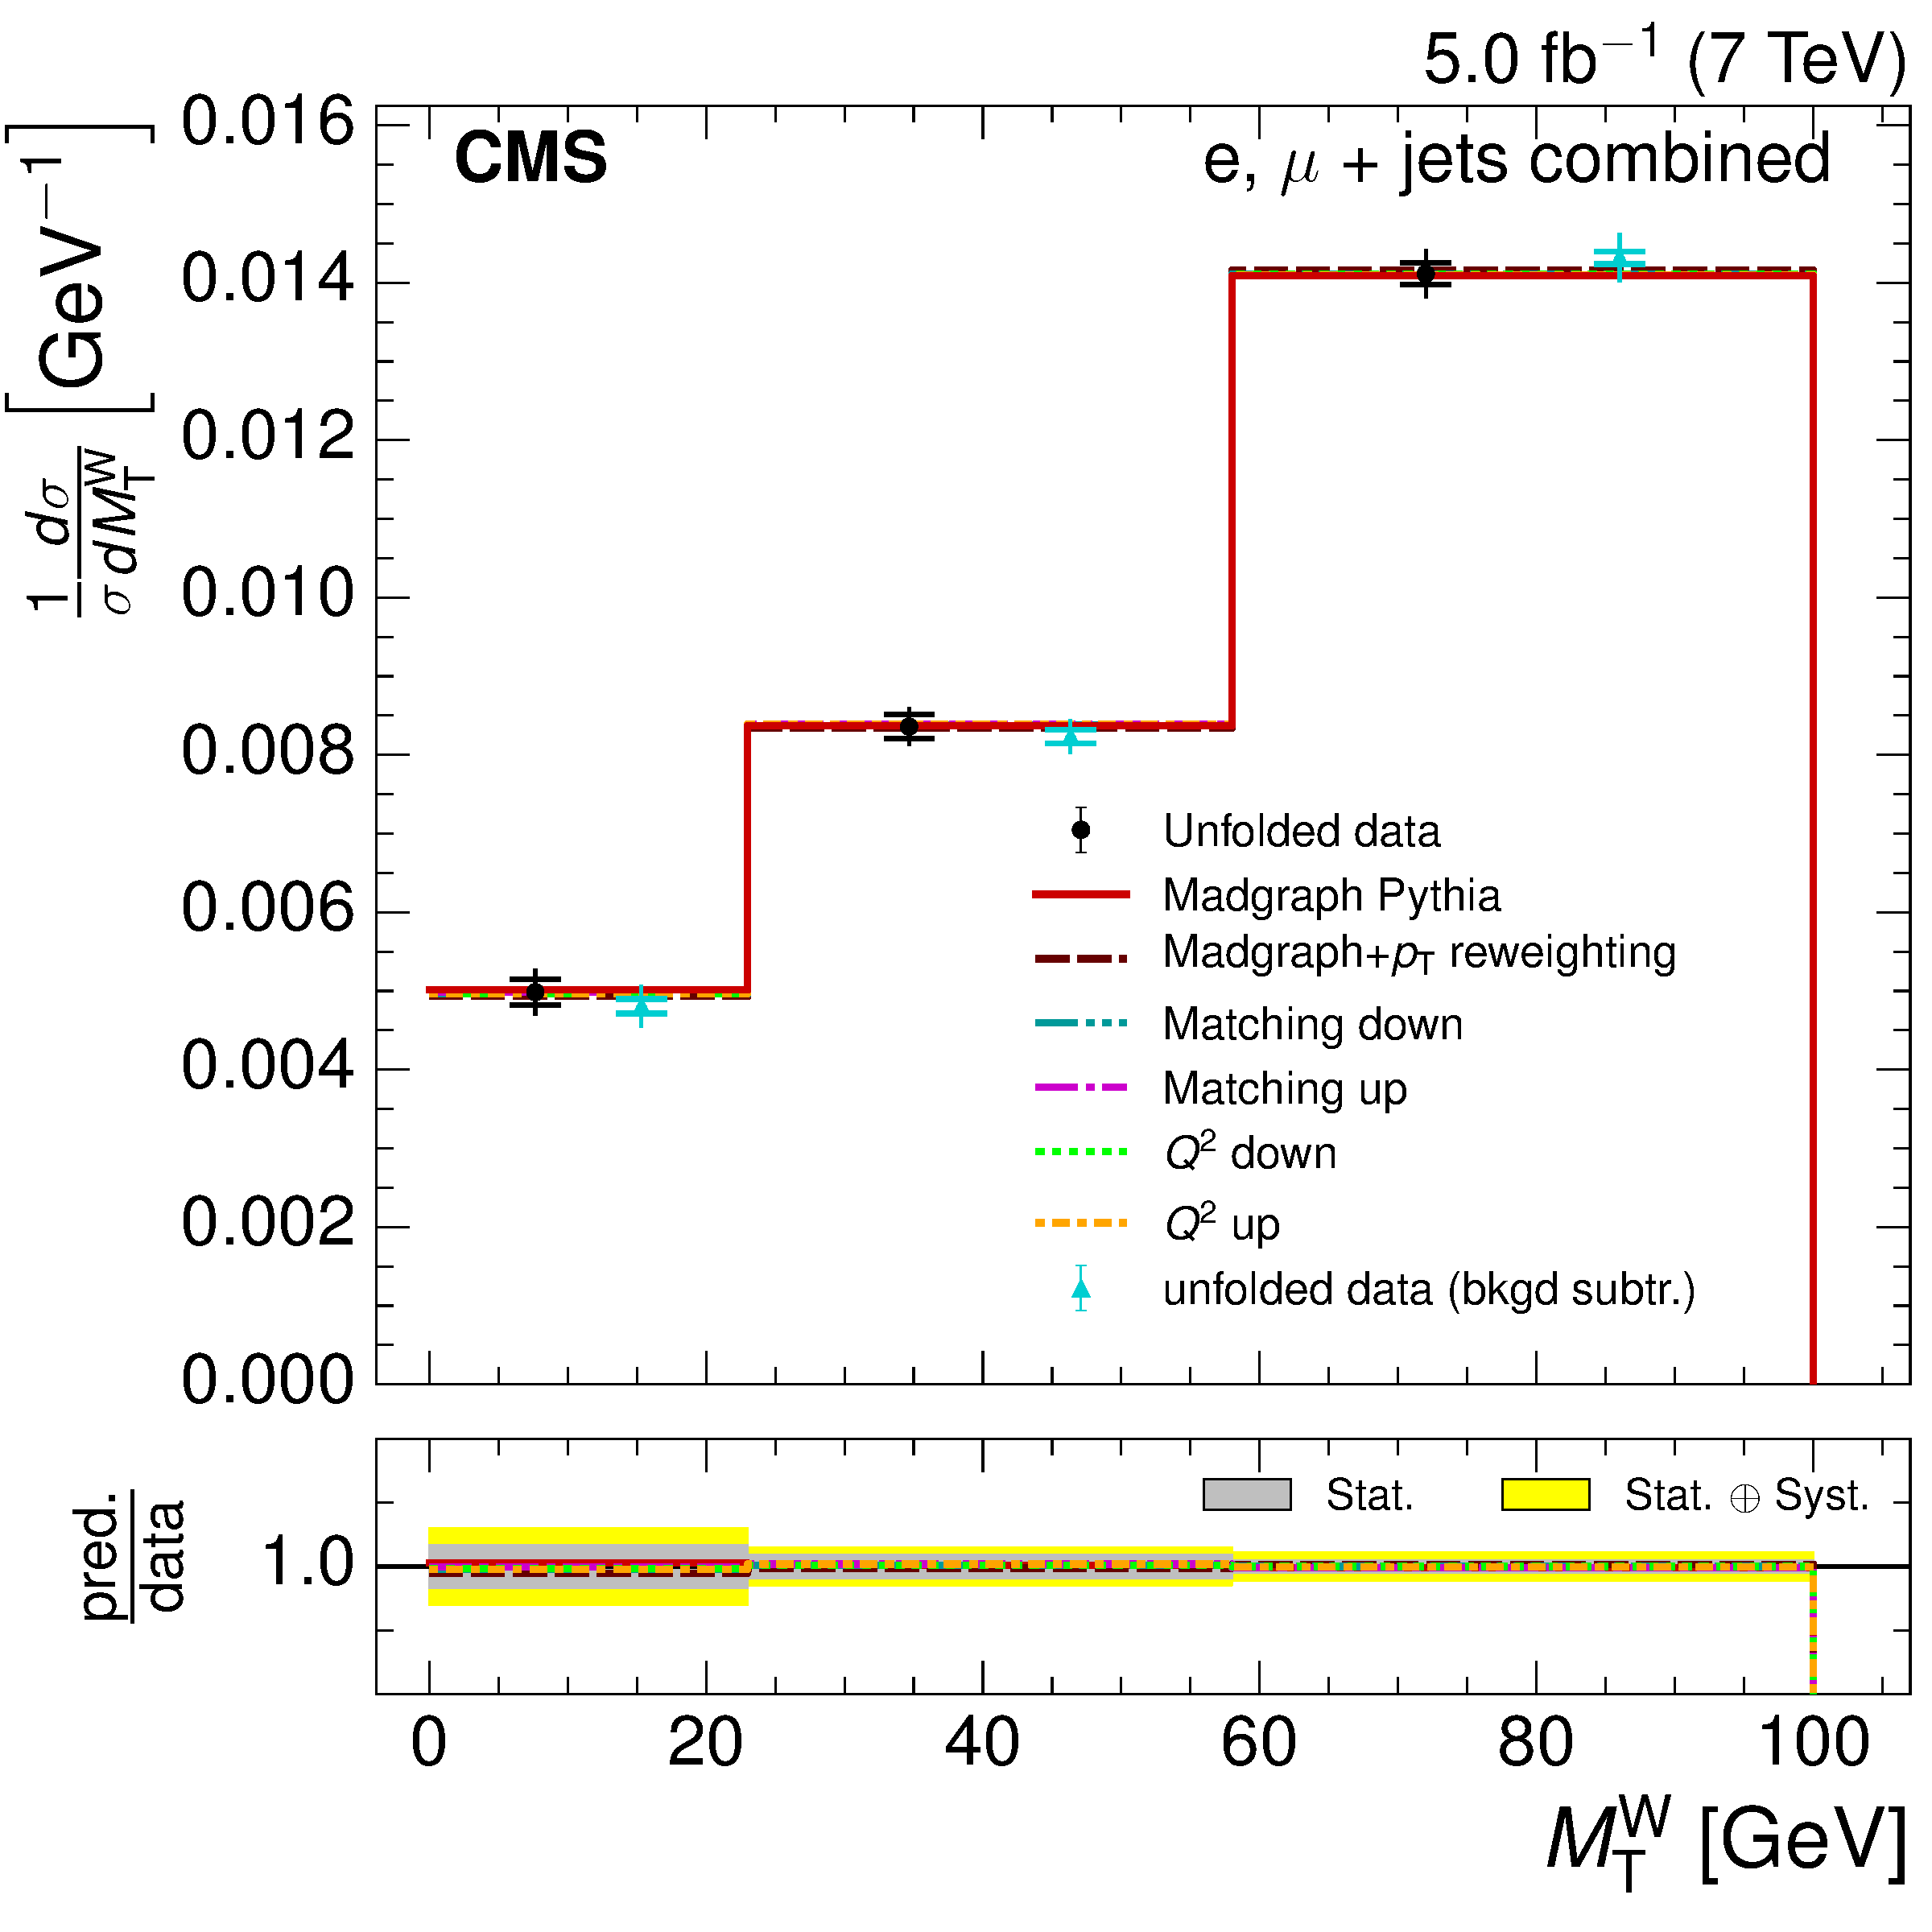
\includegraphics[width=0.32\textwidth]{Chapters/07_08_09_Analysis/Images/results/fit/7TeV/MT/central/normalised_xsection_combined_systematics_shifts_with_bkgd_subtraction_results.pdf}\\
     \caption[Comparison of the measured normalised differential cross section, with background
     subtraction resutls, with respect to \met, \HT, \st, \wpt and \mt to different Monte Carlo generators and
     predictions at $\roots=7\TeV$.]{Comparison of the measured normalised differential cross section,
     including from the background subtraction method, with respect to \met, \HT, \st, \wpt and \mt to
     different Monte Carlo generators: \MADGRAPH, \POWHEGHERWIG, \POWHEGPYTHIA and \MADGRAPH corrected for
     top \pt mismodelling (left) and to different Monte Carlo predictions matching threshold up/down and
     factorisation scale up/down (right) in the combined electron+jets and muon+jets channel at
     $\roots=7\TeV$. The lower plots show the ratio of the predictions to the data.}
     \label{fig:result_with_background_subtraction_7TeV_combined}
\end{figure}

\FloatBarrier

\subsection{8~\TeV}
\label{as:8TeV_results_tables}
%% ============================================================
% Results for MET variable, combined channel, k-value None, met type patType1CorrectedPFMet, 2orMoreBtags b-tag region
%% ============================================================
\begin{table}[htbp]
\setlength{\tabcolsep}{2pt}
\centering
\caption{Normalised \ttbar cross section measurement with respect to \MET variable
at a centre-of-mass energy of 8 TeV (combination of electron and muon channels). The errors shown are combined statistical, fit and unfolding errors ($^\dagger$) and systematic uncertainty ($^\star$).}
\label{tab:MET_xsections_8TeV_combined}
\begin{tabular}{lrrrr}
\hline
$\ensuremath{E_{\mathrm{T}}^{\mathrm{miss}}}$ bin [\GeV] & \multicolumn{4}{c}{$\sigma_{meas} \left(\times 10^{3}\right)$}\\ 
\hline
0--27~\GeV &  $6.62$ & $ \pm~ 0.07^\dagger$ & $ \pm~ 0.58^\star$ & $(8.82\%)$\\ 
27--52~\GeV &  $13.47$ & $ \pm~ 0.09^\dagger$ & $ \pm~ 0.54^\star$ & $(4.05\%)$\\ 
52--87~\GeV &  $8.76$ & $ \pm~ 0.07^\dagger$ & $ \pm~ 0.30^\star$ & $(3.57\%)$\\ 
87--130~\GeV &  $3.00$ & $ \pm~ 0.03^\dagger$ & $ \pm~ 0.27^\star$ & $(9.19\%)$\\ 
130--172~\GeV &  $0.80$ & $ \pm~ 0.01^\dagger$ & $ \pm~ 0.11^\star$ & $(14.21\%)$\\ 
$\geq 172$~\GeV &  $0.12$ & $ \pm~ 0.00^\dagger$ & $ \pm~ 0.02^\star$ & $(21.14\%)$\\ 
\hline 
\end{tabular}
\end{table}

%% ============================================================
% Results for HT variable, combined channel, k-value None, met type patType1CorrectedPFMet, 2orMoreBtags b-tag region
%% ============================================================
\begin{table}[htbp]
\setlength{\tabcolsep}{2pt}
\centering
\caption{Normalised \ttbar cross section measurement with respect to \HT variable
at a centre-of-mass energy of 8 TeV (combination of electron and muon channels). The errors shown are combined statistical, fit and unfolding errors ($^\dagger$) and systematic uncertainty ($^\star$).}
\label{tab:HT_xsections_8TeV_combined}
\begin{tabular}{lrrrr}
\hline
$\ensuremath{H_{\mathrm{T}}}$ bin [\GeV] & \multicolumn{4}{c}{$\sigma_{meas} \left(\times 10^{3}\right)$}\\ 
\hline
120--185~\GeV &  $2.15$ & $ \pm~ 0.02^\dagger$ & $ \pm~ 0.22^\star$ & $(10.14\%)$\\ 
185--215~\GeV &  $4.35$ & $ \pm~ 0.04^\dagger$ & $ \pm~ 0.27^\star$ & $(6.33\%)$\\ 
215--247~\GeV &  $4.58$ & $ \pm~ 0.04^\dagger$ & $ \pm~ 0.19^\star$ & $(4.20\%)$\\ 
247--283~\GeV &  $3.98$ & $ \pm~ 0.03^\dagger$ & $ \pm~ 0.13^\star$ & $(3.34\%)$\\ 
283--323~\GeV &  $3.08$ & $ \pm~ 0.02^\dagger$ & $ \pm~ 0.13^\star$ & $(4.43\%)$\\ 
323--365~\GeV &  $2.23$ & $ \pm~ 0.02^\dagger$ & $ \pm~ 0.11^\star$ & $(4.94\%)$\\ 
365--409~\GeV &  $1.55$ & $ \pm~ 0.01^\dagger$ & $ \pm~ 0.10^\star$ & $(6.19\%)$\\ 
409--458~\GeV &  $1.03$ & $ \pm~ 0.01^\dagger$ & $ \pm~ 0.09^\star$ & $(8.27\%)$\\ 
458--512~\GeV &  $0.66$ & $ \pm~ 0.01^\dagger$ & $ \pm~ 0.06^\star$ & $(9.18\%)$\\ 
512--570~\GeV &  $0.41$ & $ \pm~ 0.00^\dagger$ & $ \pm~ 0.04^\star$ & $(9.72\%)$\\ 
570--629~\GeV &  $0.26$ & $ \pm~ 0.00^\dagger$ & $ \pm~ 0.03^\star$ & $(10.79\%)$\\ 
629--691~\GeV &  $0.16$ & $ \pm~ 0.00^\dagger$ & $ \pm~ 0.02^\star$ & $(9.96\%)$\\ 
691--769~\GeV &  $0.10$ & $ \pm~ 0.00^\dagger$ & $ \pm~ 0.01^\star$ & $(10.77\%)$\\ 
$\geq 769$~\GeV &  $0.05$ & $ \pm~ 0.00^\dagger$ & $ \pm~ 0.01^\star$ & $(12.87\%)$\\ 
\hline 
\end{tabular}
\end{table}

%% ============================================================
% Results for ST variable, combined channel, k-value None, met type patType1CorrectedPFMet, 2orMoreBtags b-tag region
%% ============================================================
\begin{table}[htbp]
\setlength{\tabcolsep}{2pt}
\centering
\caption{Normalised \ttbar cross section measurement with respect to \ST variable
at a centre-of-mass energy of 8 TeV (combination of electron and muon channels). The errors shown are combined statistical, fit and unfolding errors ($^\dagger$) and systematic uncertainty ($^\star$).}
\label{tab:ST_xsections_8TeV_combined}
\begin{tabular}{lrrrr}
\hline
$\ensuremath{S_{\mathrm{T}}}$ bin [\GeV] & \multicolumn{4}{c}{$\sigma_{meas} \left(\times 10^{3}\right)$}\\ 
\hline
146--277~\GeV &  $1.12$ & $ \pm~ 0.02^\dagger$ & $ \pm~ 0.09^\star$ & $(8.48\%)$\\ 
277--319~\GeV &  $3.64$ & $ \pm~ 0.05^\dagger$ & $ \pm~ 0.22^\star$ & $(6.33\%)$\\ 
319--361~\GeV &  $3.83$ & $ \pm~ 0.04^\dagger$ & $ \pm~ 0.18^\star$ & $(4.79\%)$\\ 
361--408~\GeV &  $3.22$ & $ \pm~ 0.03^\dagger$ & $ \pm~ 0.09^\star$ & $(2.83\%)$\\ 
408--459~\GeV &  $2.38$ & $ \pm~ 0.02^\dagger$ & $ \pm~ 0.08^\star$ & $(3.58\%)$\\ 
459--514~\GeV &  $1.64$ & $ \pm~ 0.02^\dagger$ & $ \pm~ 0.11^\star$ & $(6.90\%)$\\ 
514--573~\GeV &  $1.05$ & $ \pm~ 0.01^\dagger$ & $ \pm~ 0.10^\star$ & $(9.88\%)$\\ 
573--637~\GeV &  $0.66$ & $ \pm~ 0.01^\dagger$ & $ \pm~ 0.07^\star$ & $(10.99\%)$\\ 
637--705~\GeV &  $0.40$ & $ \pm~ 0.00^\dagger$ & $ \pm~ 0.05^\star$ & $(11.52\%)$\\ 
705--774~\GeV &  $0.24$ & $ \pm~ 0.00^\dagger$ & $ \pm~ 0.03^\star$ & $(12.47\%)$\\ 
774--854~\GeV &  $0.14$ & $ \pm~ 0.00^\dagger$ & $ \pm~ 0.02^\star$ & $(11.42\%)$\\ 
854--940~\GeV &  $0.08$ & $ \pm~ 0.00^\dagger$ & $ \pm~ 0.01^\star$ & $(10.30\%)$\\ 
$\geq 940$~\GeV &  $0.04$ & $ \pm~ 0.00^\dagger$ & $ \pm~ 0.00^\star$ & $(11.61\%)$\\ 
\hline 
\end{tabular}
\end{table}

%% ============================================================
% Results for WPT variable, combined channel, k-value None, met type patType1CorrectedPFMet, 2orMoreBtags b-tag region
%% ============================================================
\begin{table}[htbp]
\setlength{\tabcolsep}{2pt}
\centering
\caption{Normalised \ttbar cross section measurement with respect to \WPT variable
at a centre-of-mass energy of 8 TeV (combination of electron and muon channels). The errors shown are combined statistical, fit and unfolding errors ($^\dagger$) and systematic uncertainty ($^\star$).}
\label{tab:WPT_xsections_8TeV_combined}
\begin{tabular}{lrrrr}
\hline
$\ensuremath{p^{\mathrm{W}}_{\mathrm{T}}}$ bin [\GeV] & \multicolumn{4}{c}{$\sigma_{meas} \left(\times 10^{3}\right)$}\\ 
\hline
0--27~\GeV &  $3.64$ & $ \pm~ 0.03^\dagger$ & $ \pm~ 0.17^\star$ & $(4.89\%)$\\ 
27--52~\GeV &  $8.59$ & $ \pm~ 0.06^\dagger$ & $ \pm~ 0.39^\star$ & $(4.58\%)$\\ 
52--78~\GeV &  $9.22$ & $ \pm~ 0.06^\dagger$ & $ \pm~ 0.24^\star$ & $(2.63\%)$\\ 
78--105~\GeV &  $6.98$ & $ \pm~ 0.05^\dagger$ & $ \pm~ 0.10^\star$ & $(1.59\%)$\\ 
105--134~\GeV &  $4.24$ & $ \pm~ 0.04^\dagger$ & $ \pm~ 0.20^\star$ & $(4.69\%)$\\ 
134--166~\GeV &  $2.18$ & $ \pm~ 0.02^\dagger$ & $ \pm~ 0.16^\star$ & $(7.56\%)$\\ 
166--200~\GeV &  $1.01$ & $ \pm~ 0.01^\dagger$ & $ \pm~ 0.10^\star$ & $(10.06\%)$\\ 
200--237~\GeV &  $0.45$ & $ \pm~ 0.01^\dagger$ & $ \pm~ 0.06^\star$ & $(13.27\%)$\\ 
$\geq 237$~\GeV &  $0.24$ & $ \pm~ 0.00^\dagger$ & $ \pm~ 0.04^\star$ & $(17.31\%)$\\ 
\hline 
\end{tabular}
\end{table}

%% ============================================================
% Results for MT variable, combined channel, k-value None, met type patType1CorrectedPFMet, 2orMoreBtags b-tag region
%% ============================================================
\begin{table}[htbp]
\setlength{\tabcolsep}{2pt}
\centering
\caption{Normalised \ttbar cross section measurement with respect to \MT variable
at a centre-of-mass energy of 8 TeV (combination of electron and muon channels). The errors shown are combined statistical, fit and unfolding errors ($^\dagger$) and systematic uncertainty ($^\star$).}
\label{tab:MT_xsections_8TeV_combined}
\begin{tabular}{lrrrr}
\hline
$\ensuremath{M^{\mathrm{W}}_{\mathrm{T}}}$ bin [\GeV] & \multicolumn{4}{c}{$\sigma_{meas} \left(\times 10^{3}\right)$}\\ 
\hline
0--23~\GeV &  $4.88$ & $ \pm~ 0.07^\dagger$ & $ \pm~ 0.26^\star$ & $(5.52\%)$\\ 
23--58~\GeV &  $8.30$ & $ \pm~ 0.06^\dagger$ & $ \pm~ 0.22^\star$ & $(2.79\%)$\\ 
$\geq 58$~\GeV &  $14.22$ & $ \pm~ 0.06^\dagger$ & $ \pm~ 0.32^\star$ & $(2.31\%)$\\ 
\hline 
\end{tabular}
\end{table}


\begin{figure}[hbtp]
    \centering
     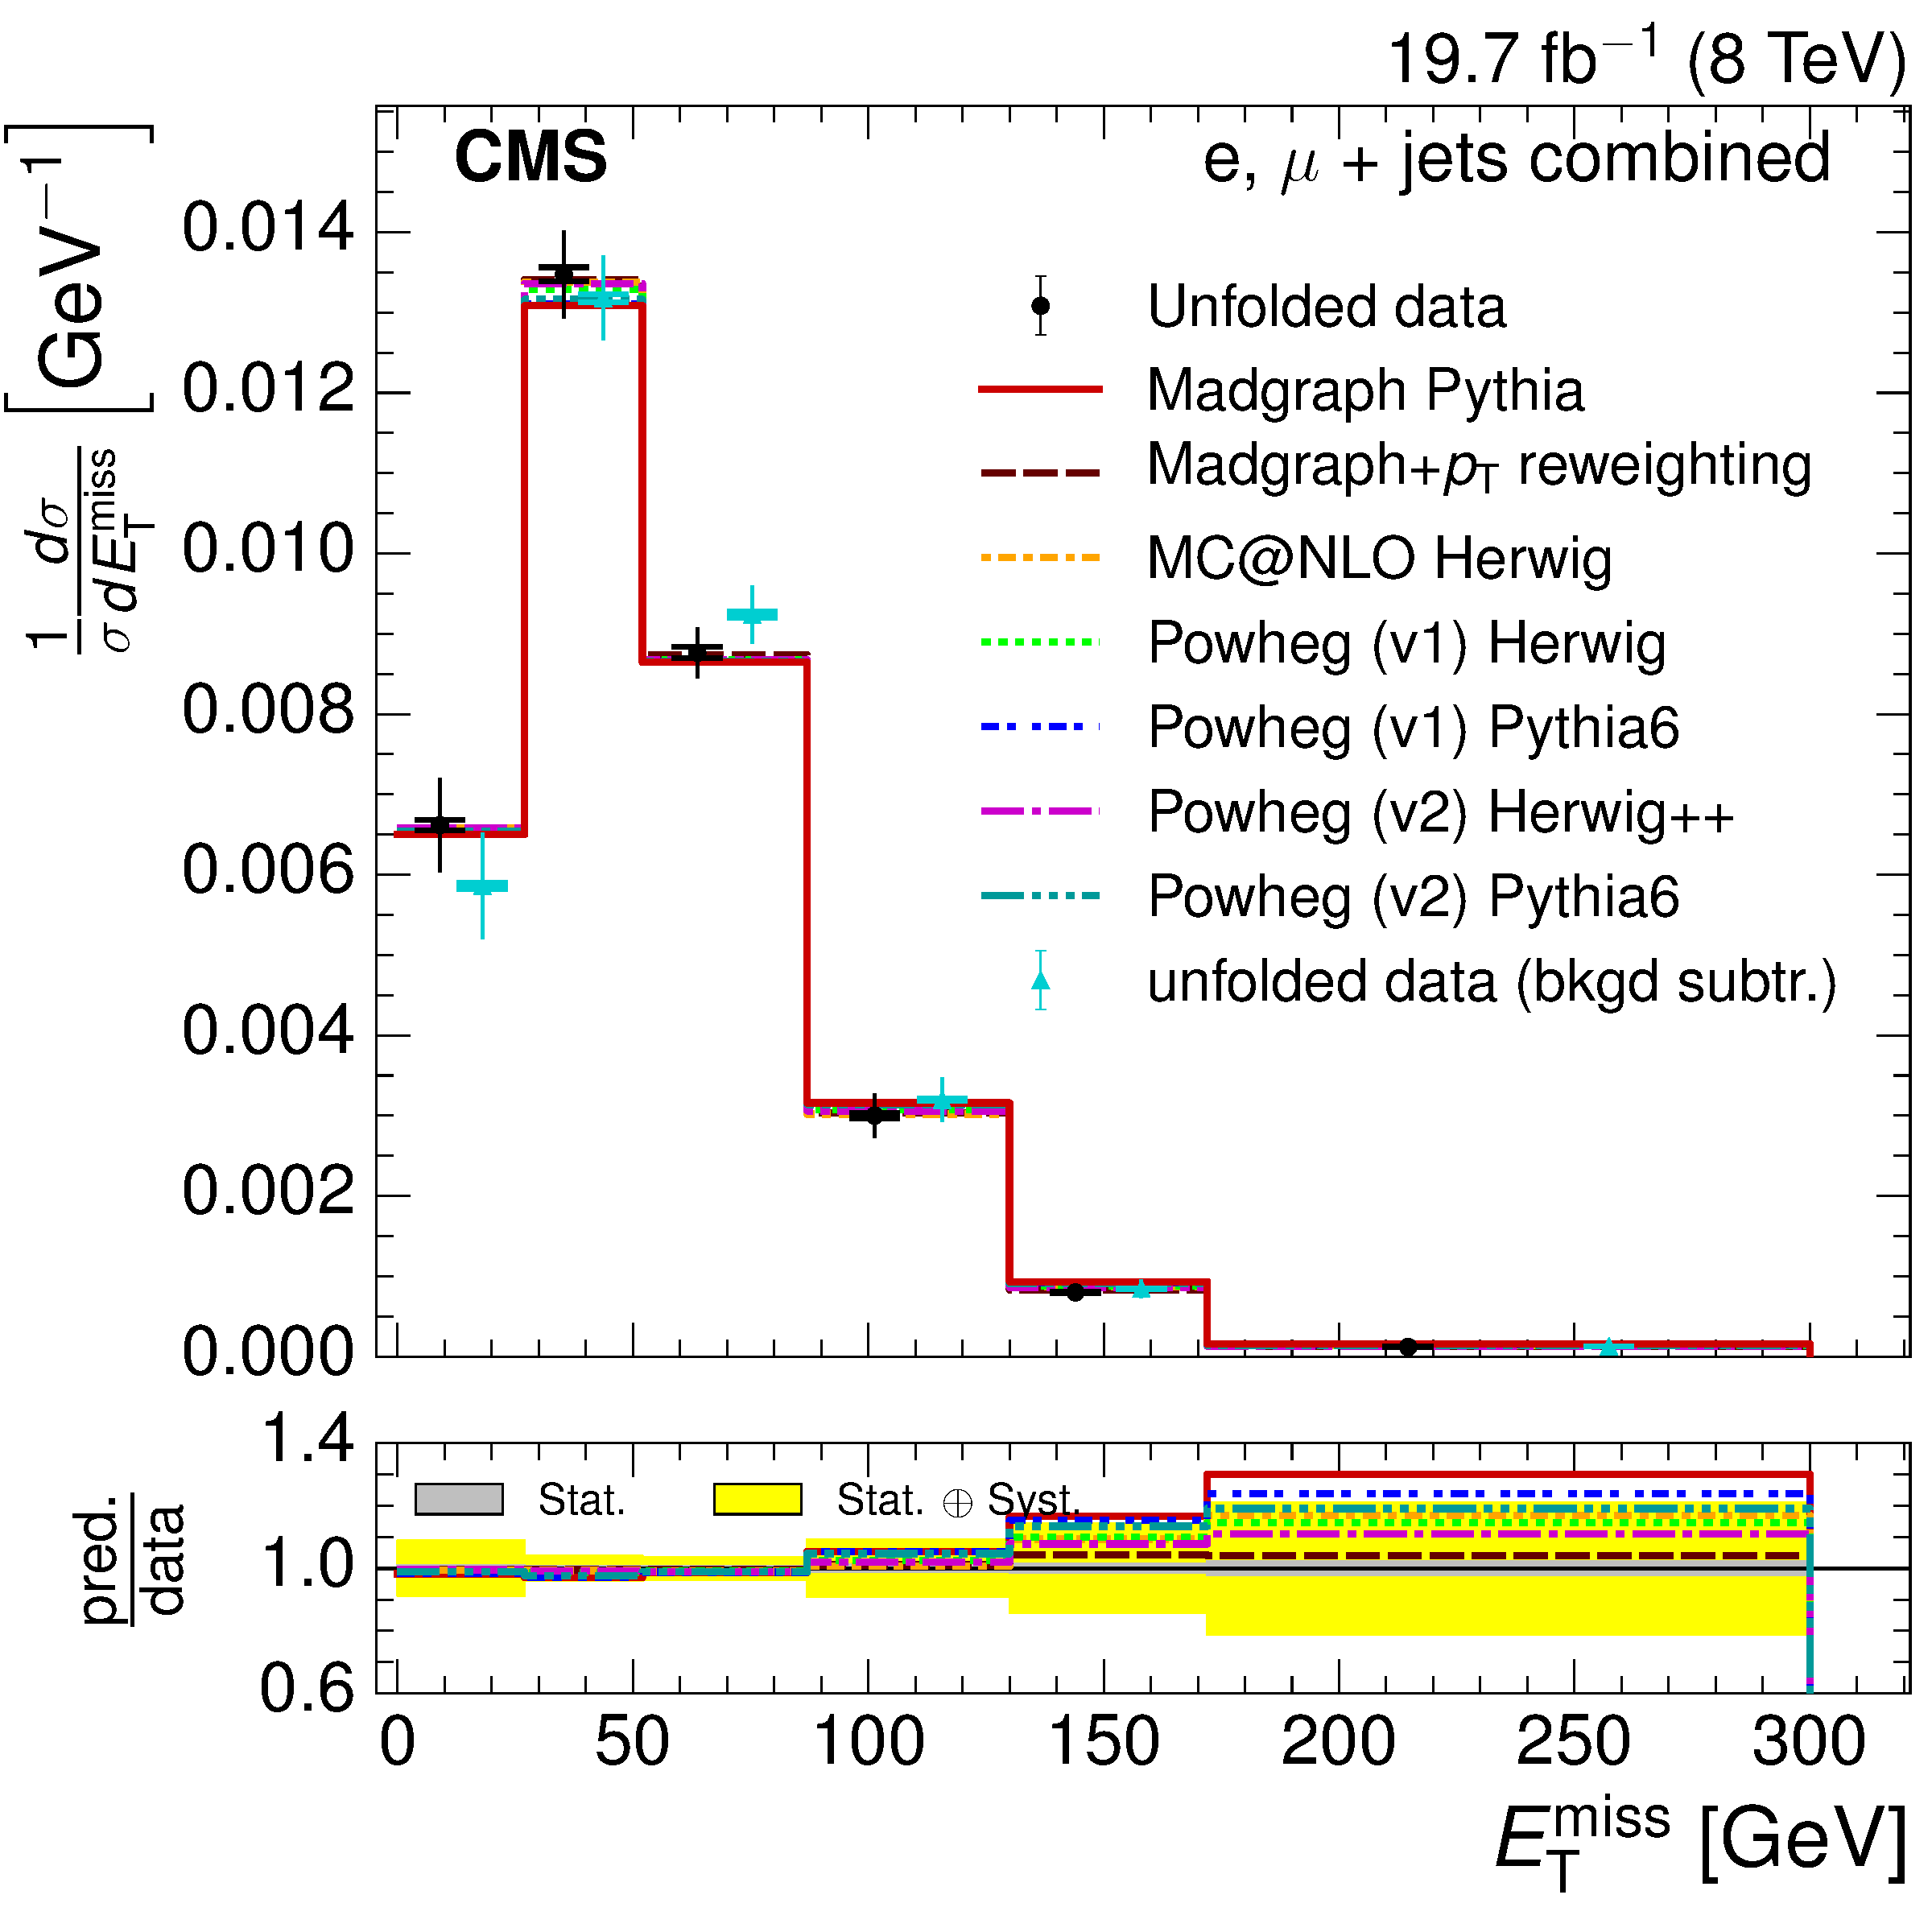
\includegraphics[width=0.32\textwidth]{Chapters/07_08_09_Analysis/Images/results/fit/8TeV/MET/central/normalised_xsection_combined_different_generators_with_bkgd_subtraction_results.pdf}\hfill
     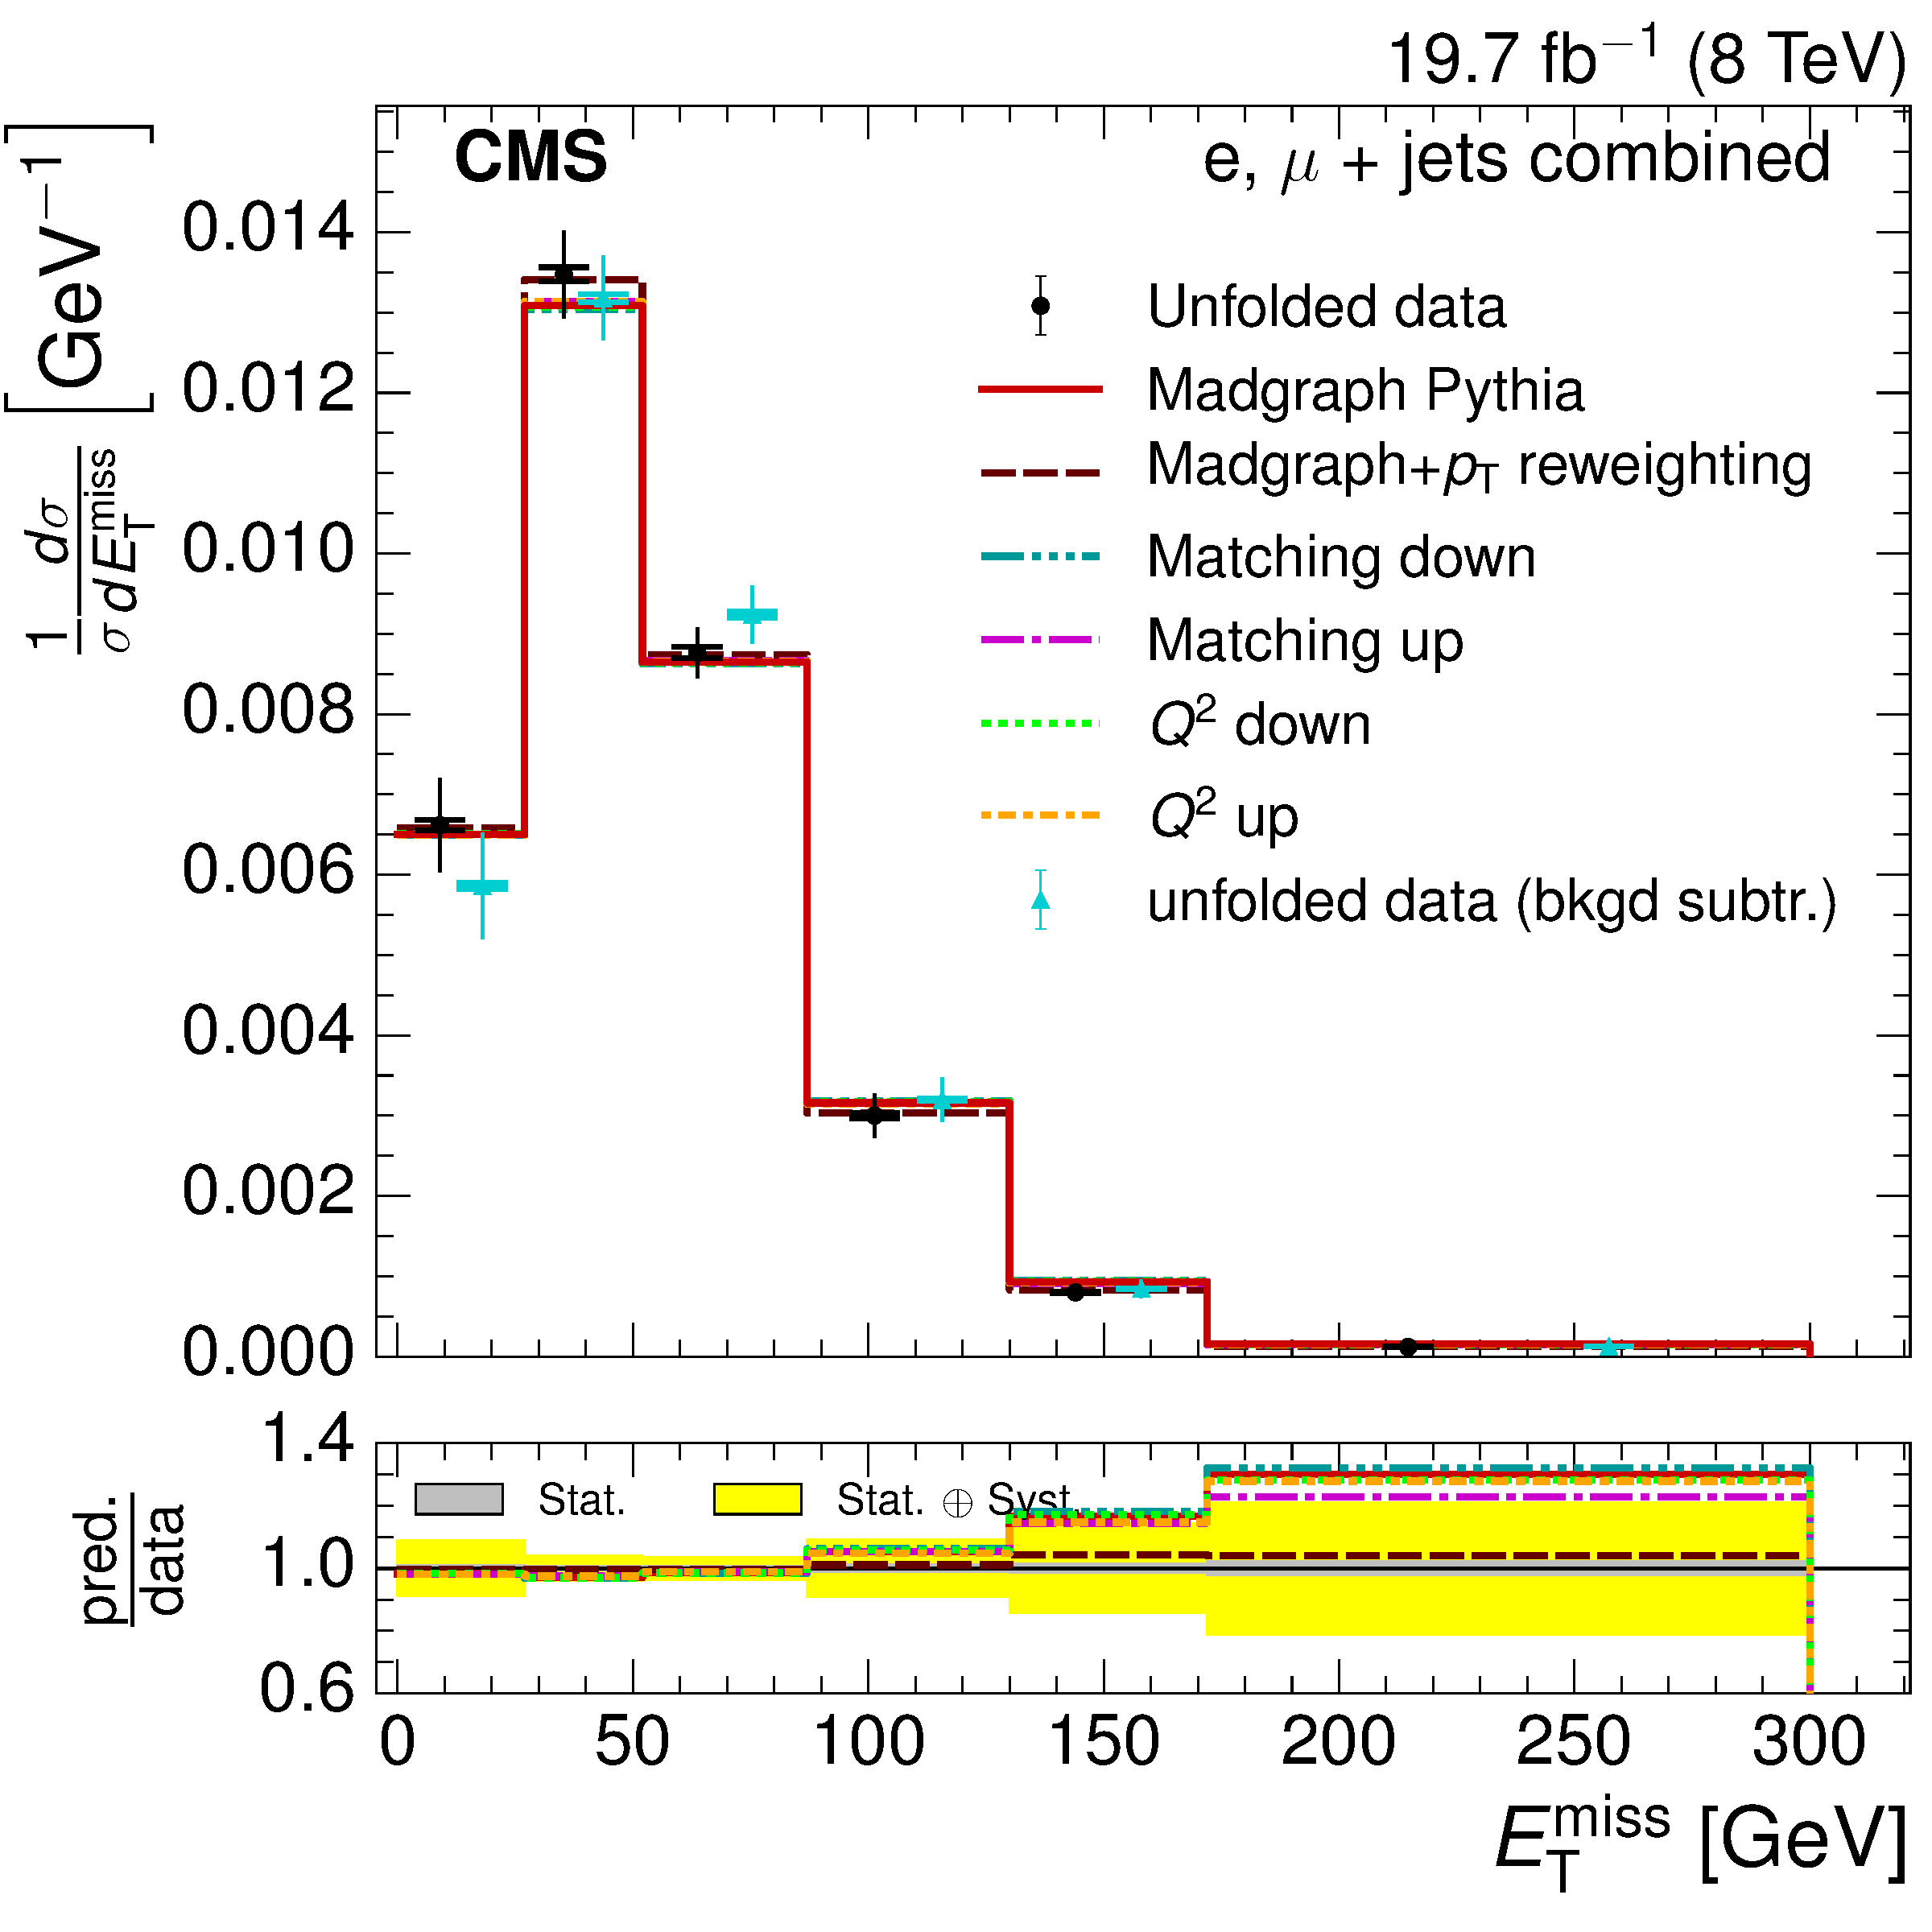
\includegraphics[width=0.32\textwidth]{Chapters/07_08_09_Analysis/Images/results/fit/8TeV/MET/central/normalised_xsection_combined_systematics_shifts_with_bkgd_subtraction_results.pdf}\\
     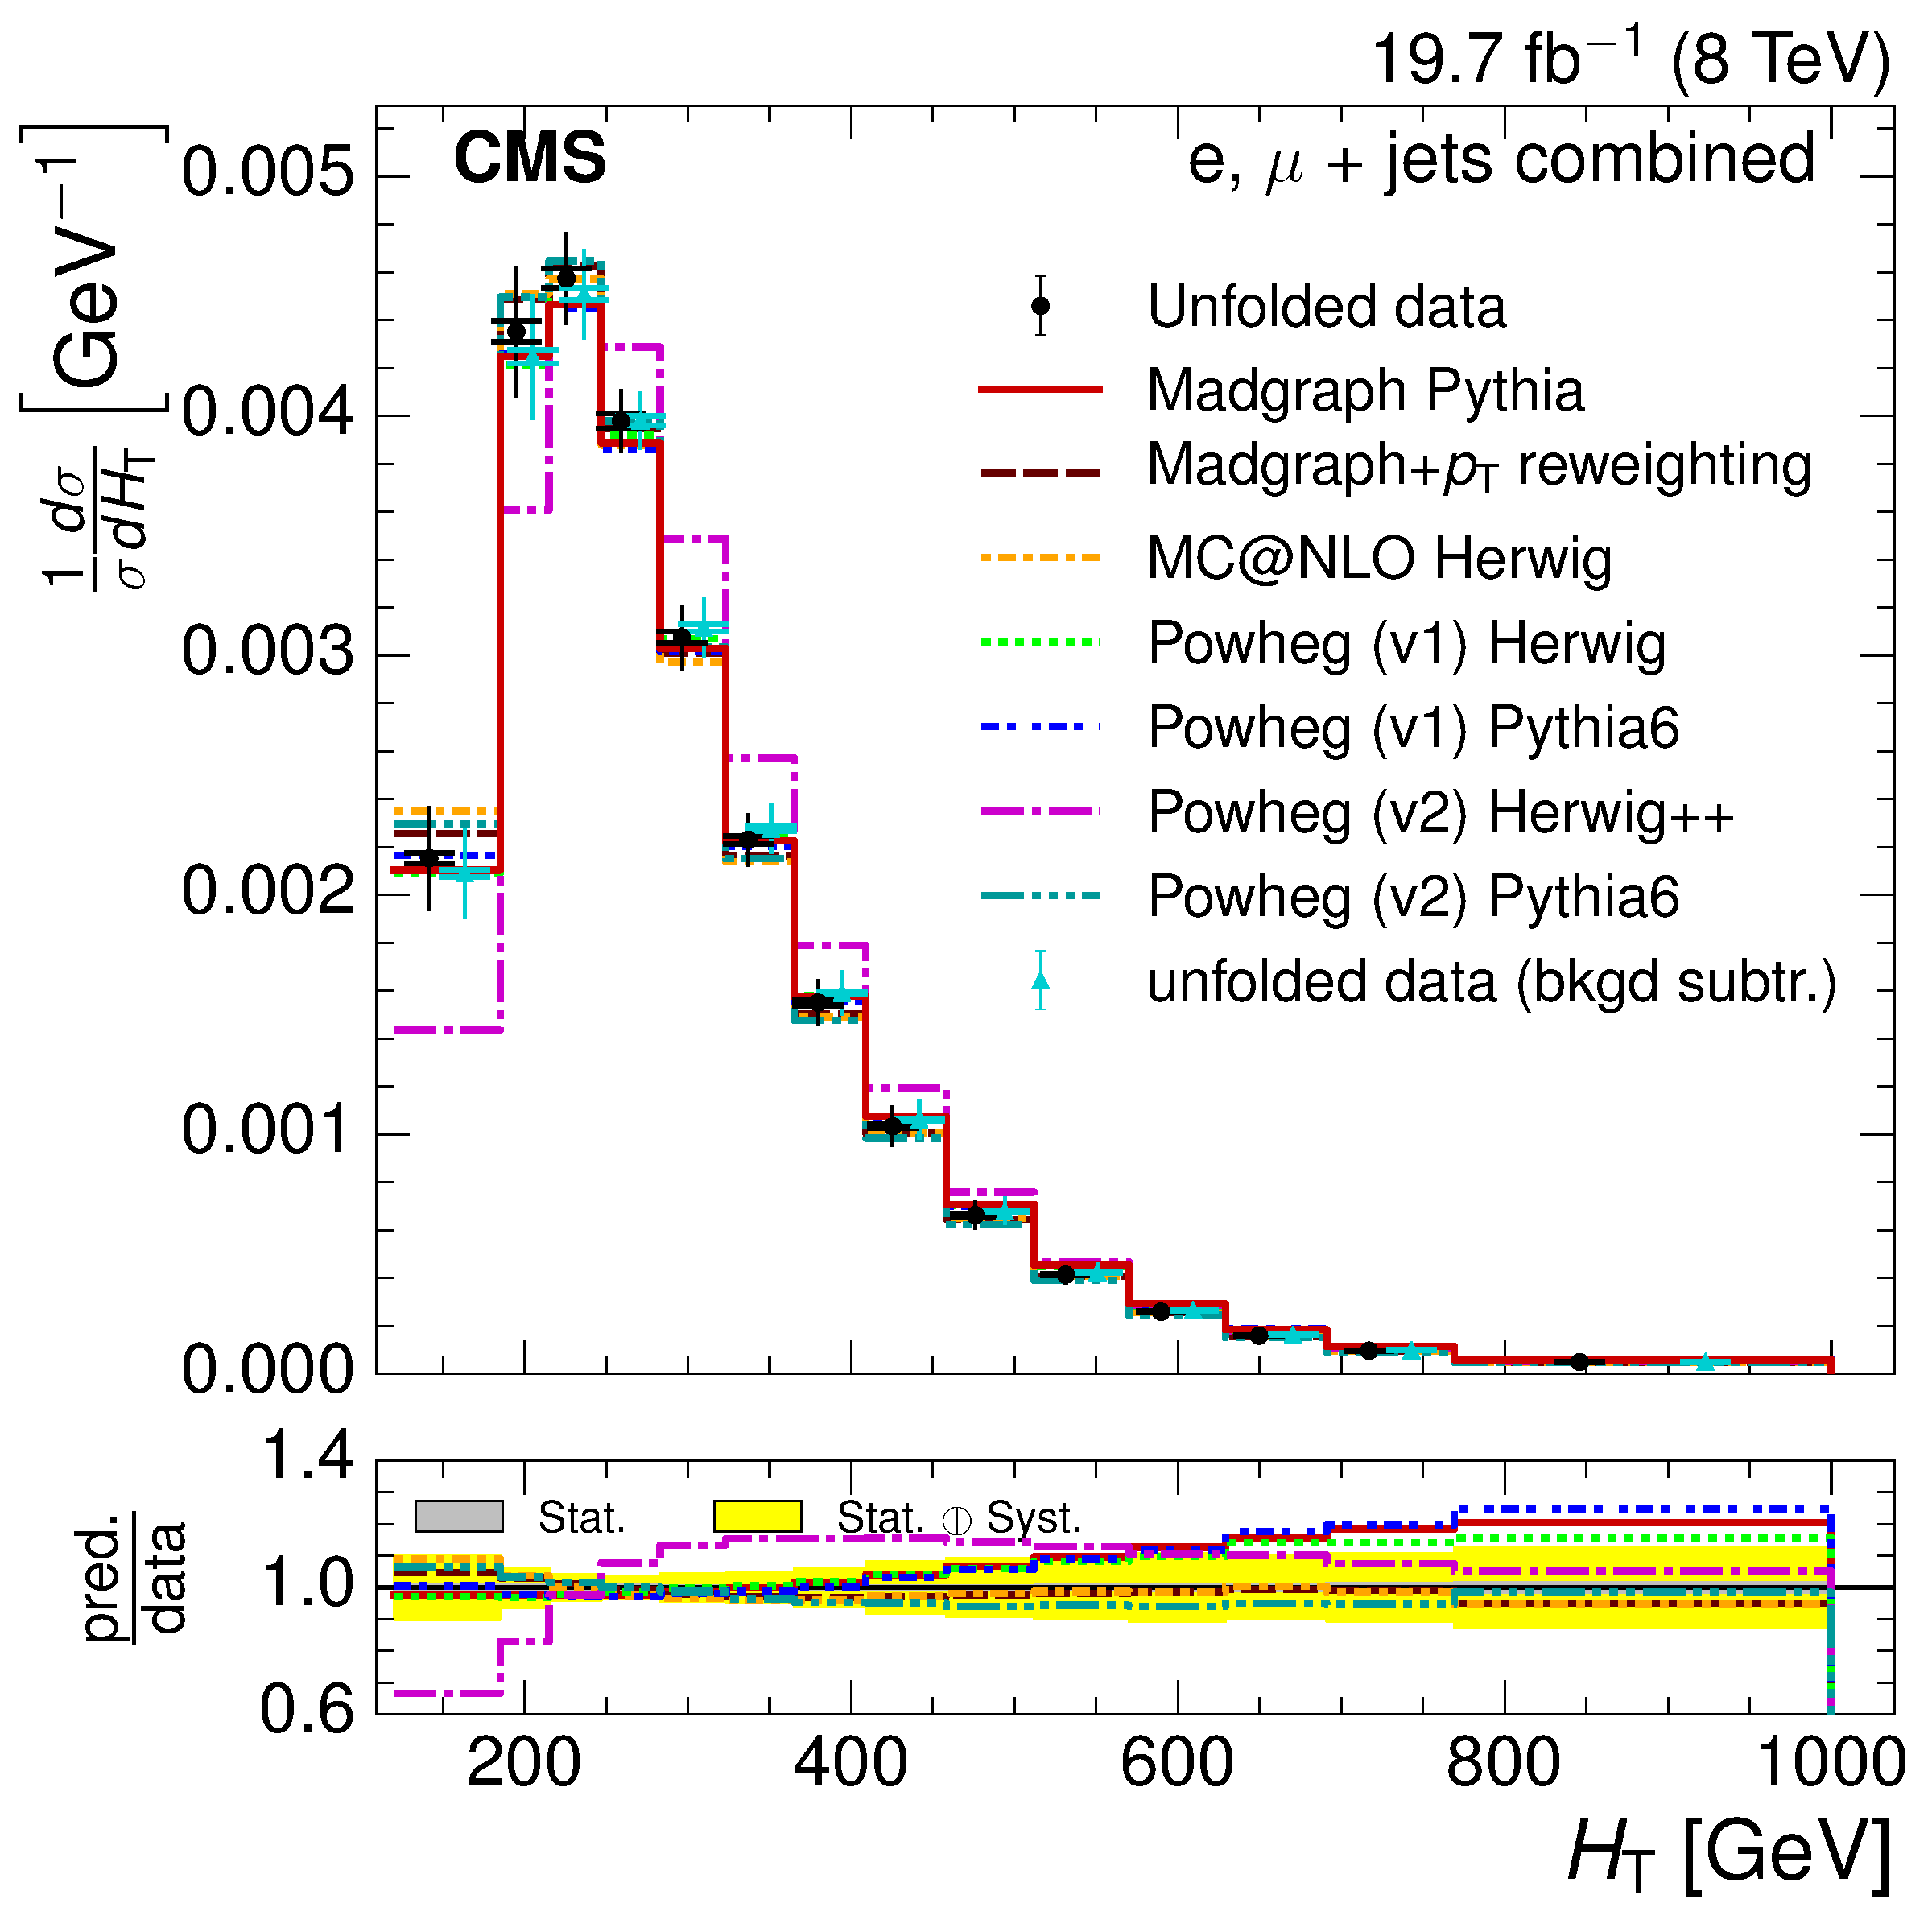
\includegraphics[width=0.32\textwidth]{Chapters/07_08_09_Analysis/Images/results/fit/8TeV/HT/central/normalised_xsection_combined_different_generators_with_bkgd_subtraction_results.pdf}\hfill
     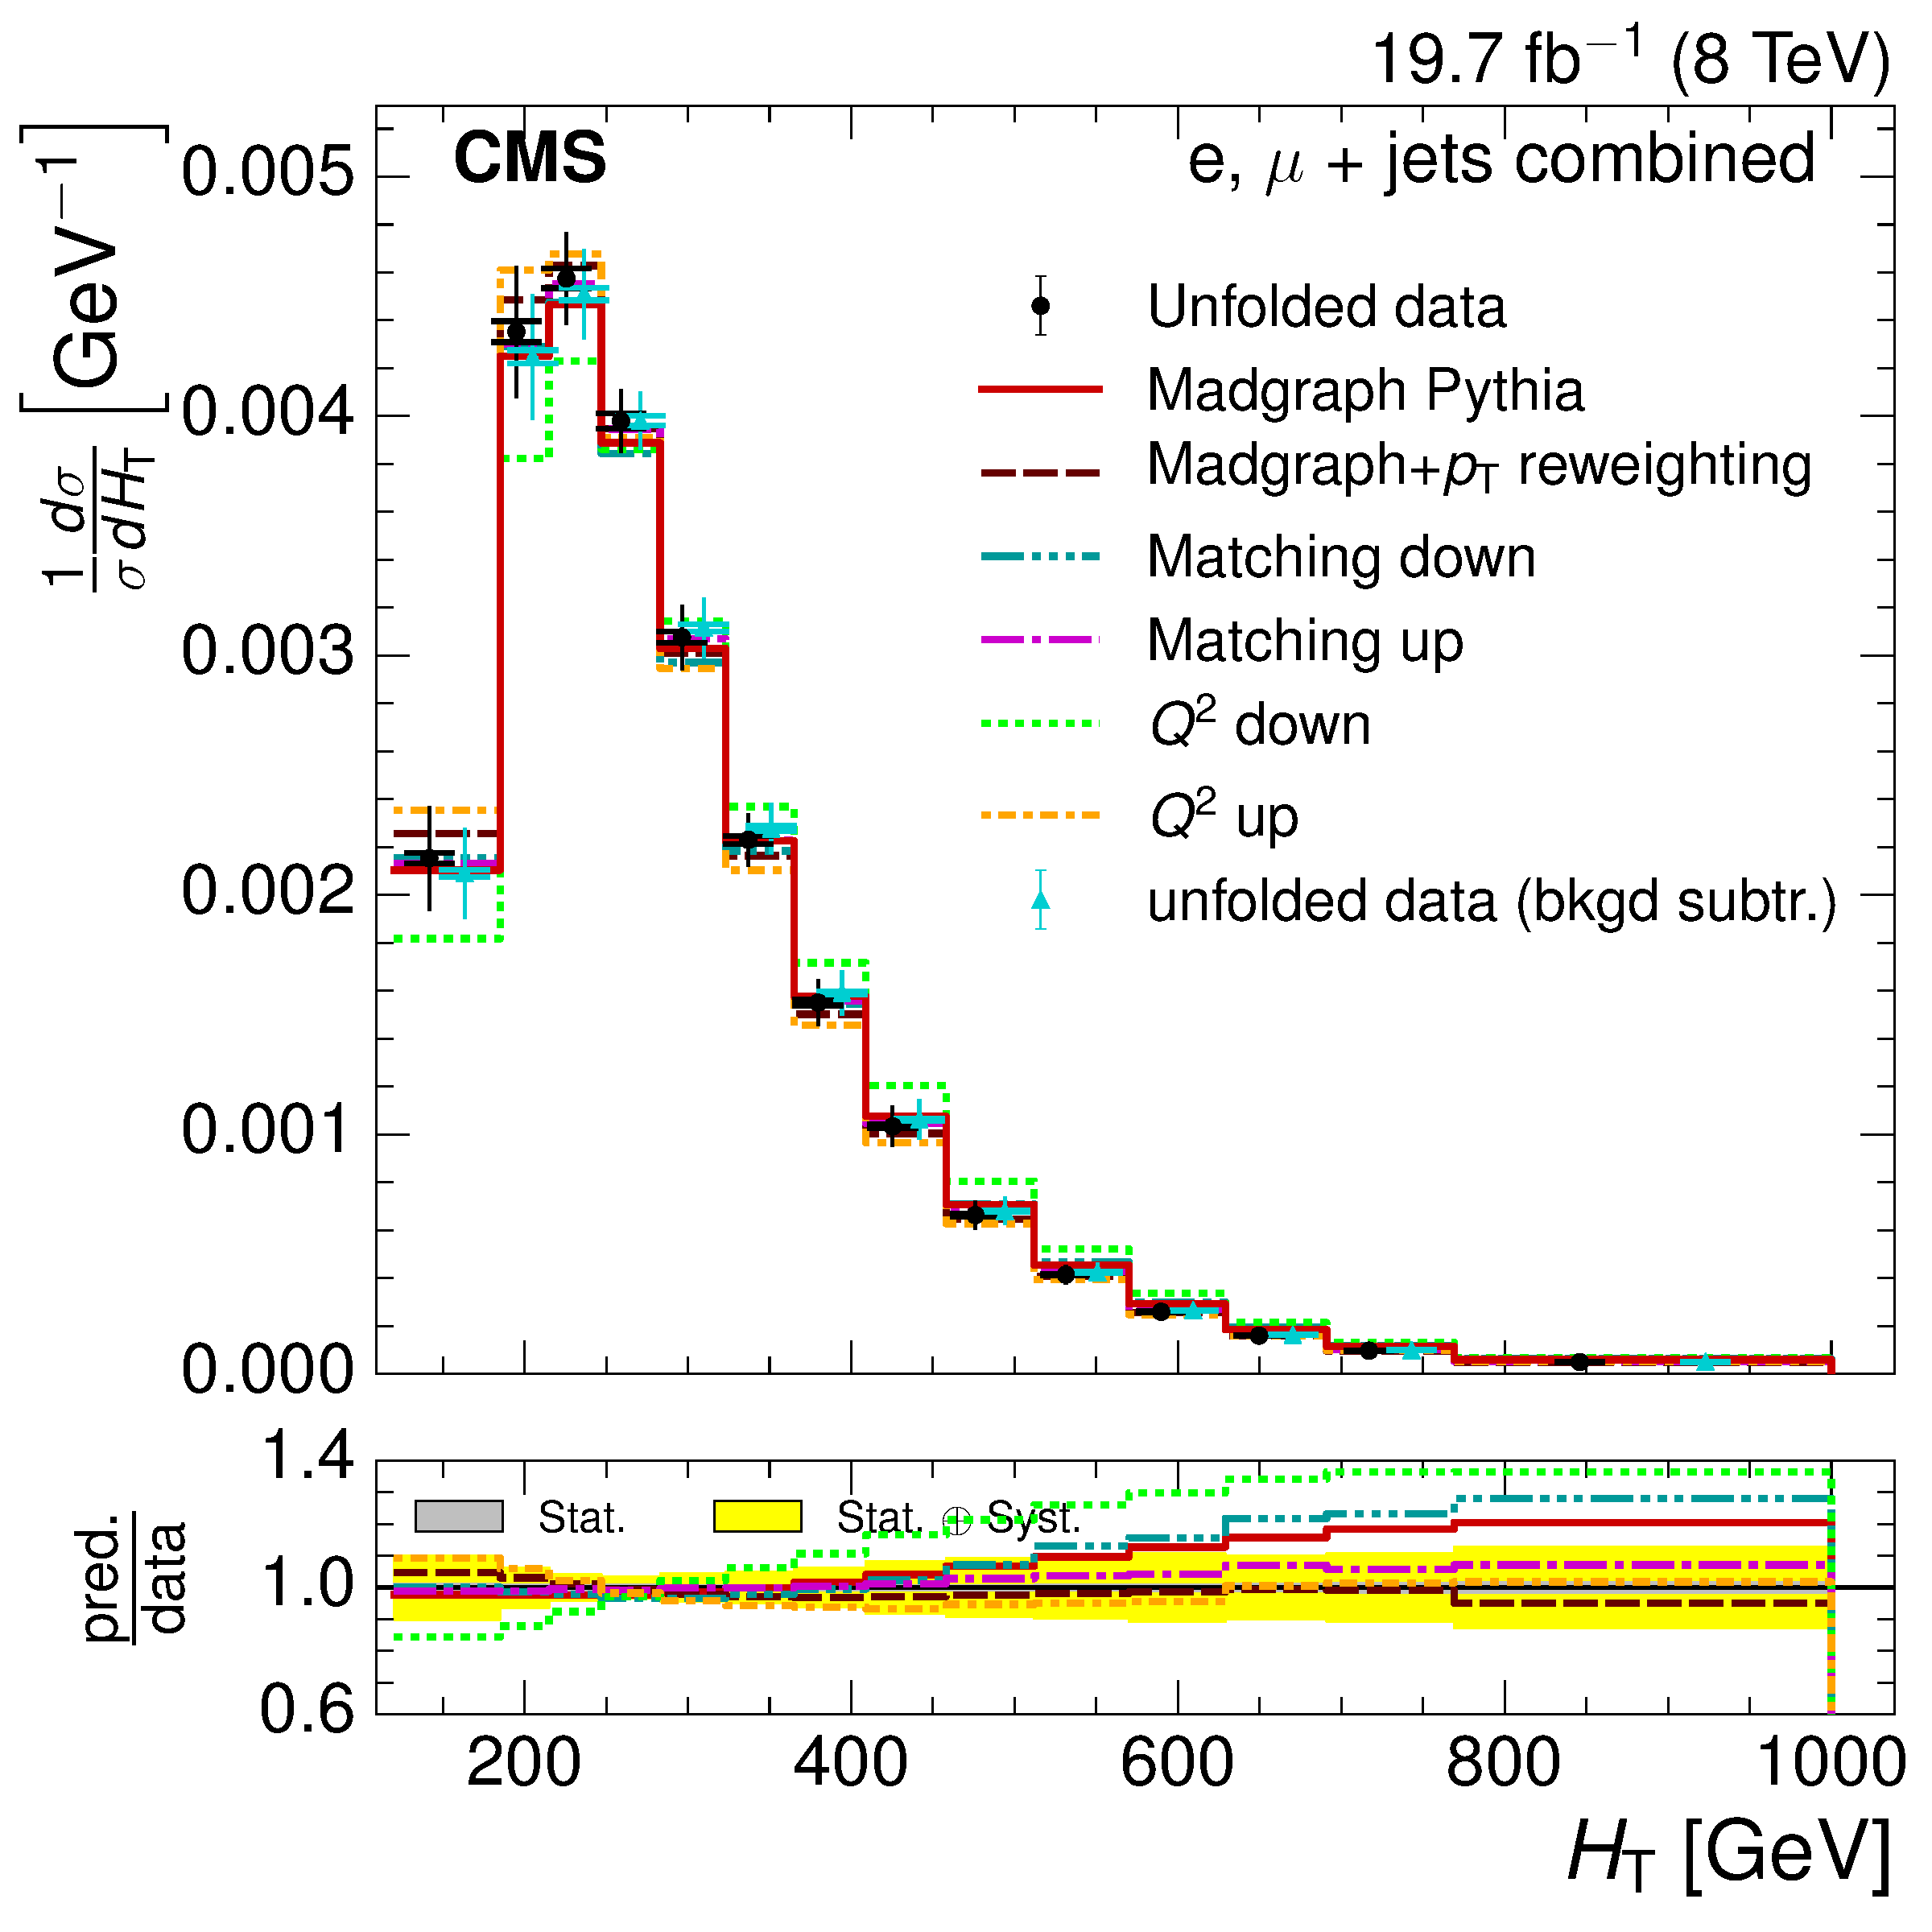
\includegraphics[width=0.32\textwidth]{Chapters/07_08_09_Analysis/Images/results/fit/8TeV/HT/central/normalised_xsection_combined_systematics_shifts_with_bkgd_subtraction_results.pdf}\\
     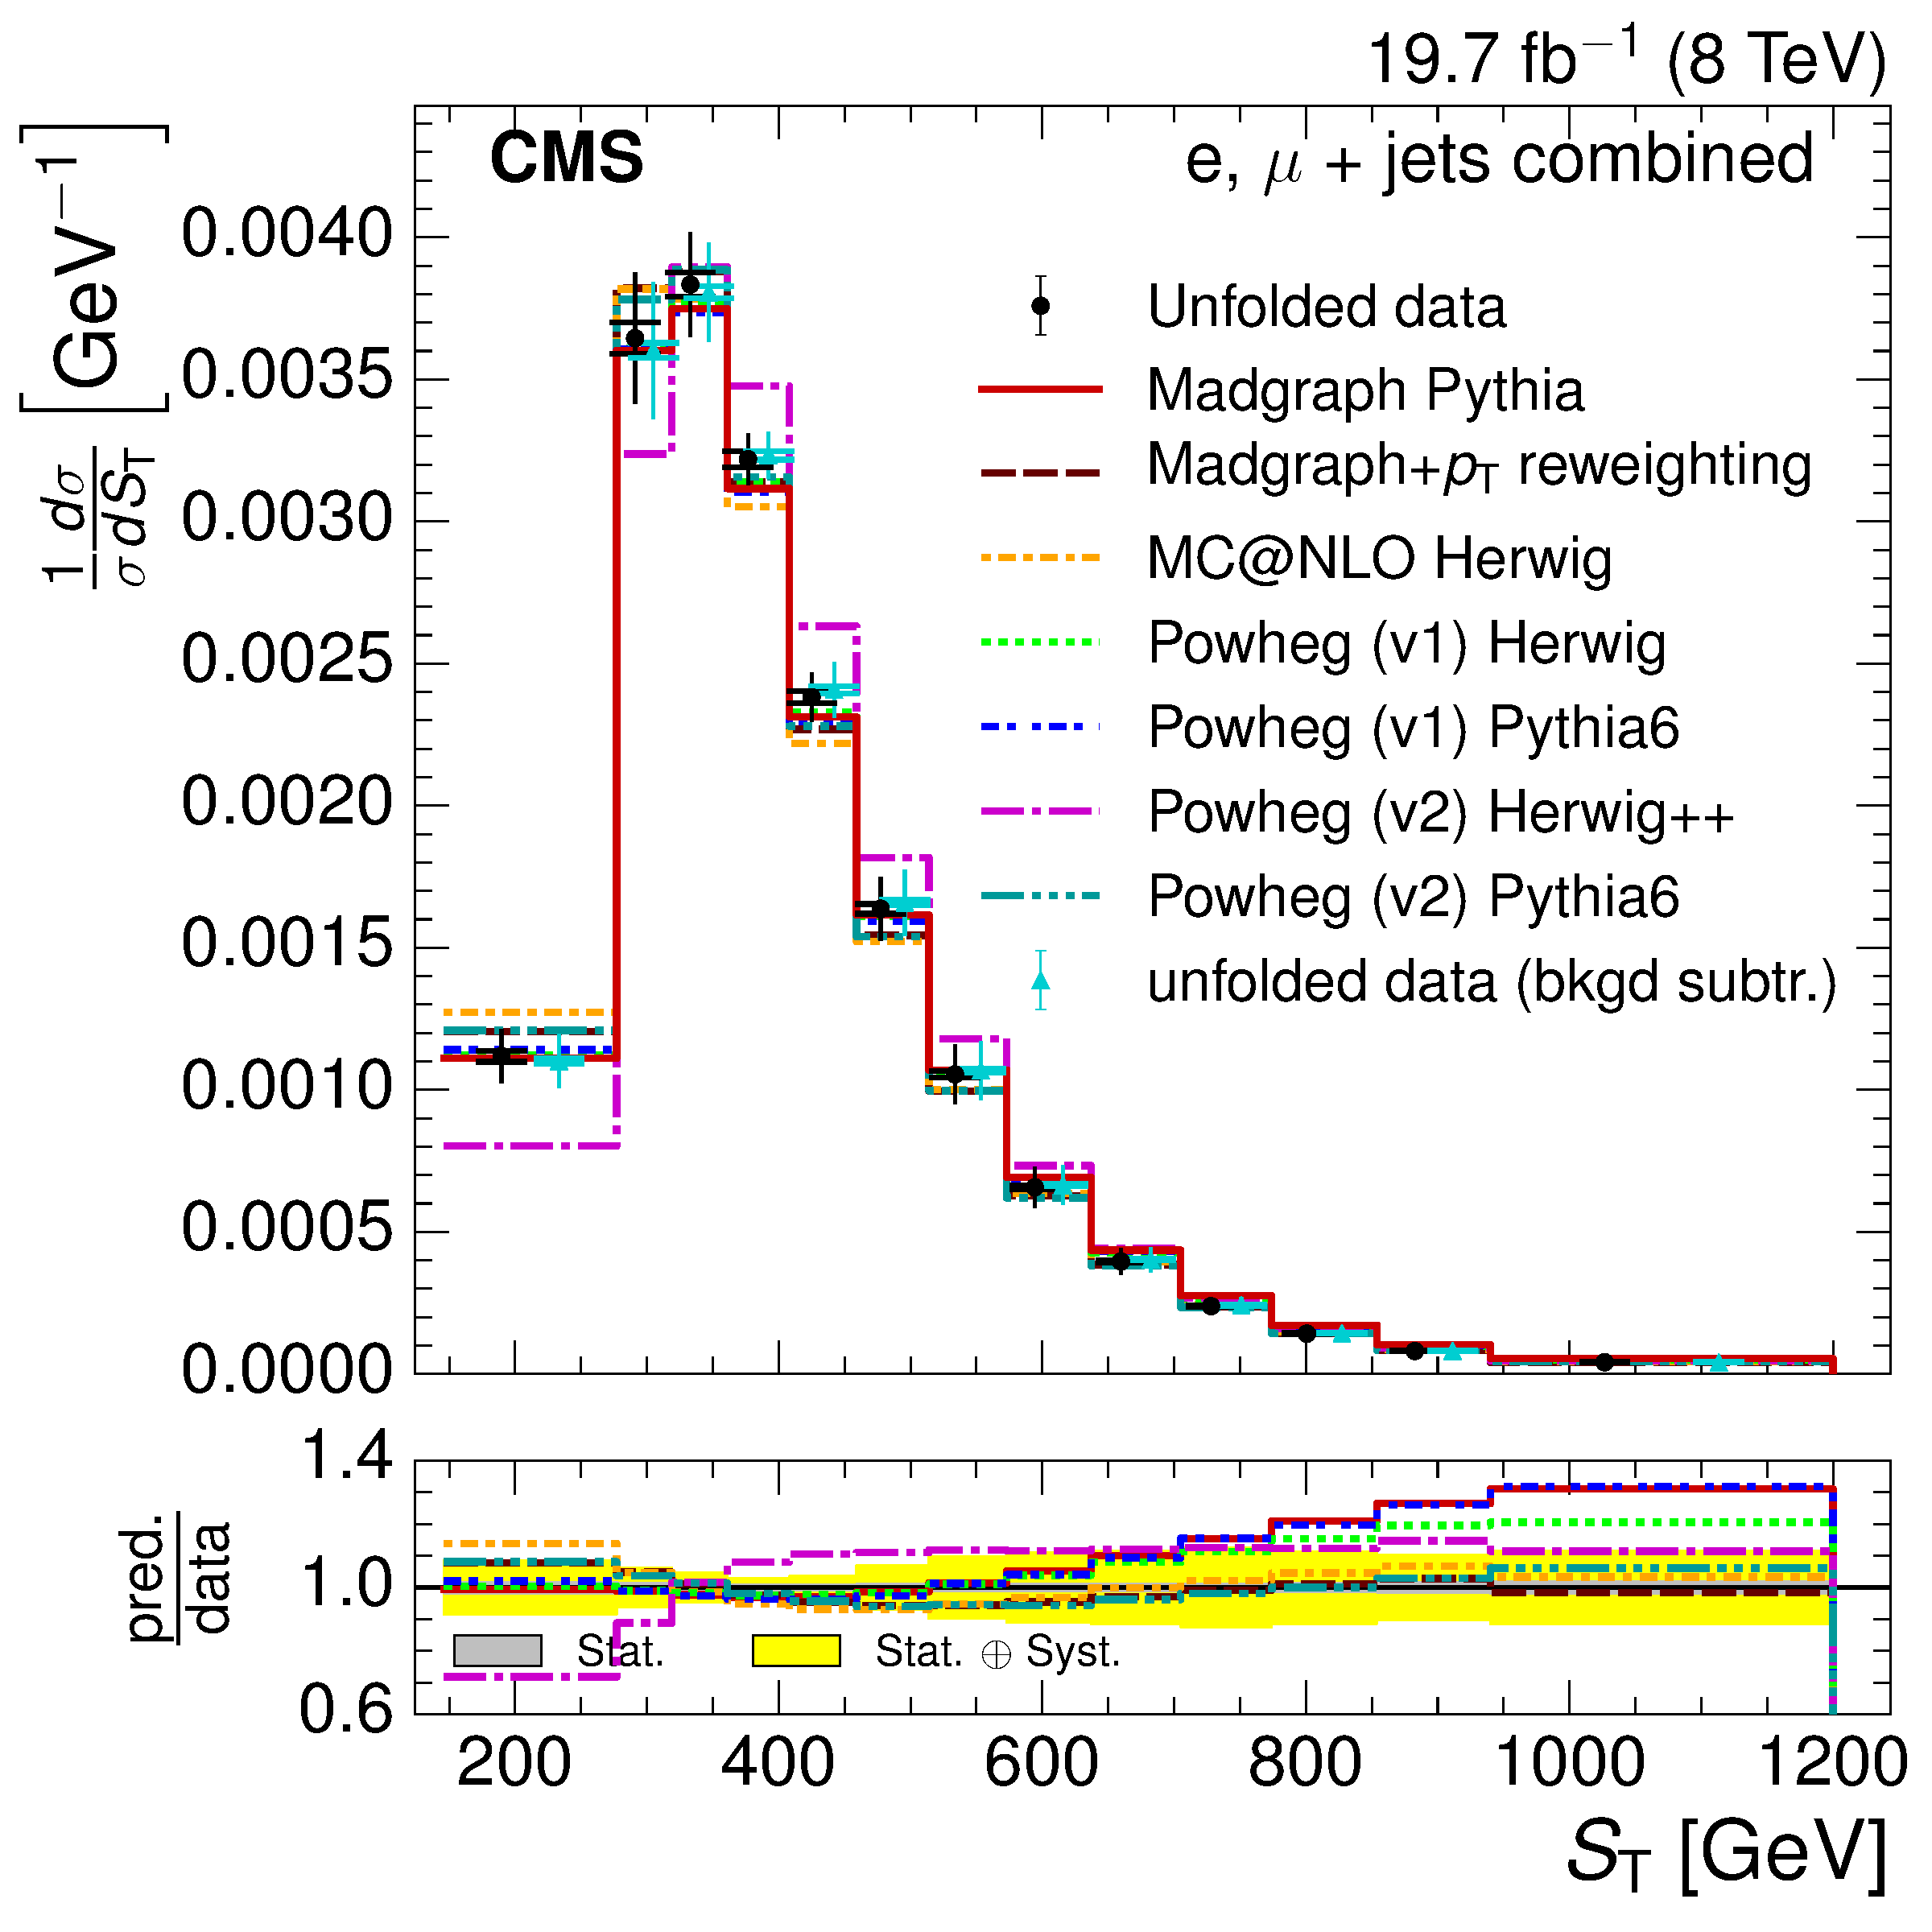
\includegraphics[width=0.32\textwidth]{Chapters/07_08_09_Analysis/Images/results/fit/8TeV/ST/central/normalised_xsection_combined_different_generators_with_bkgd_subtraction_results.pdf}\hfill
     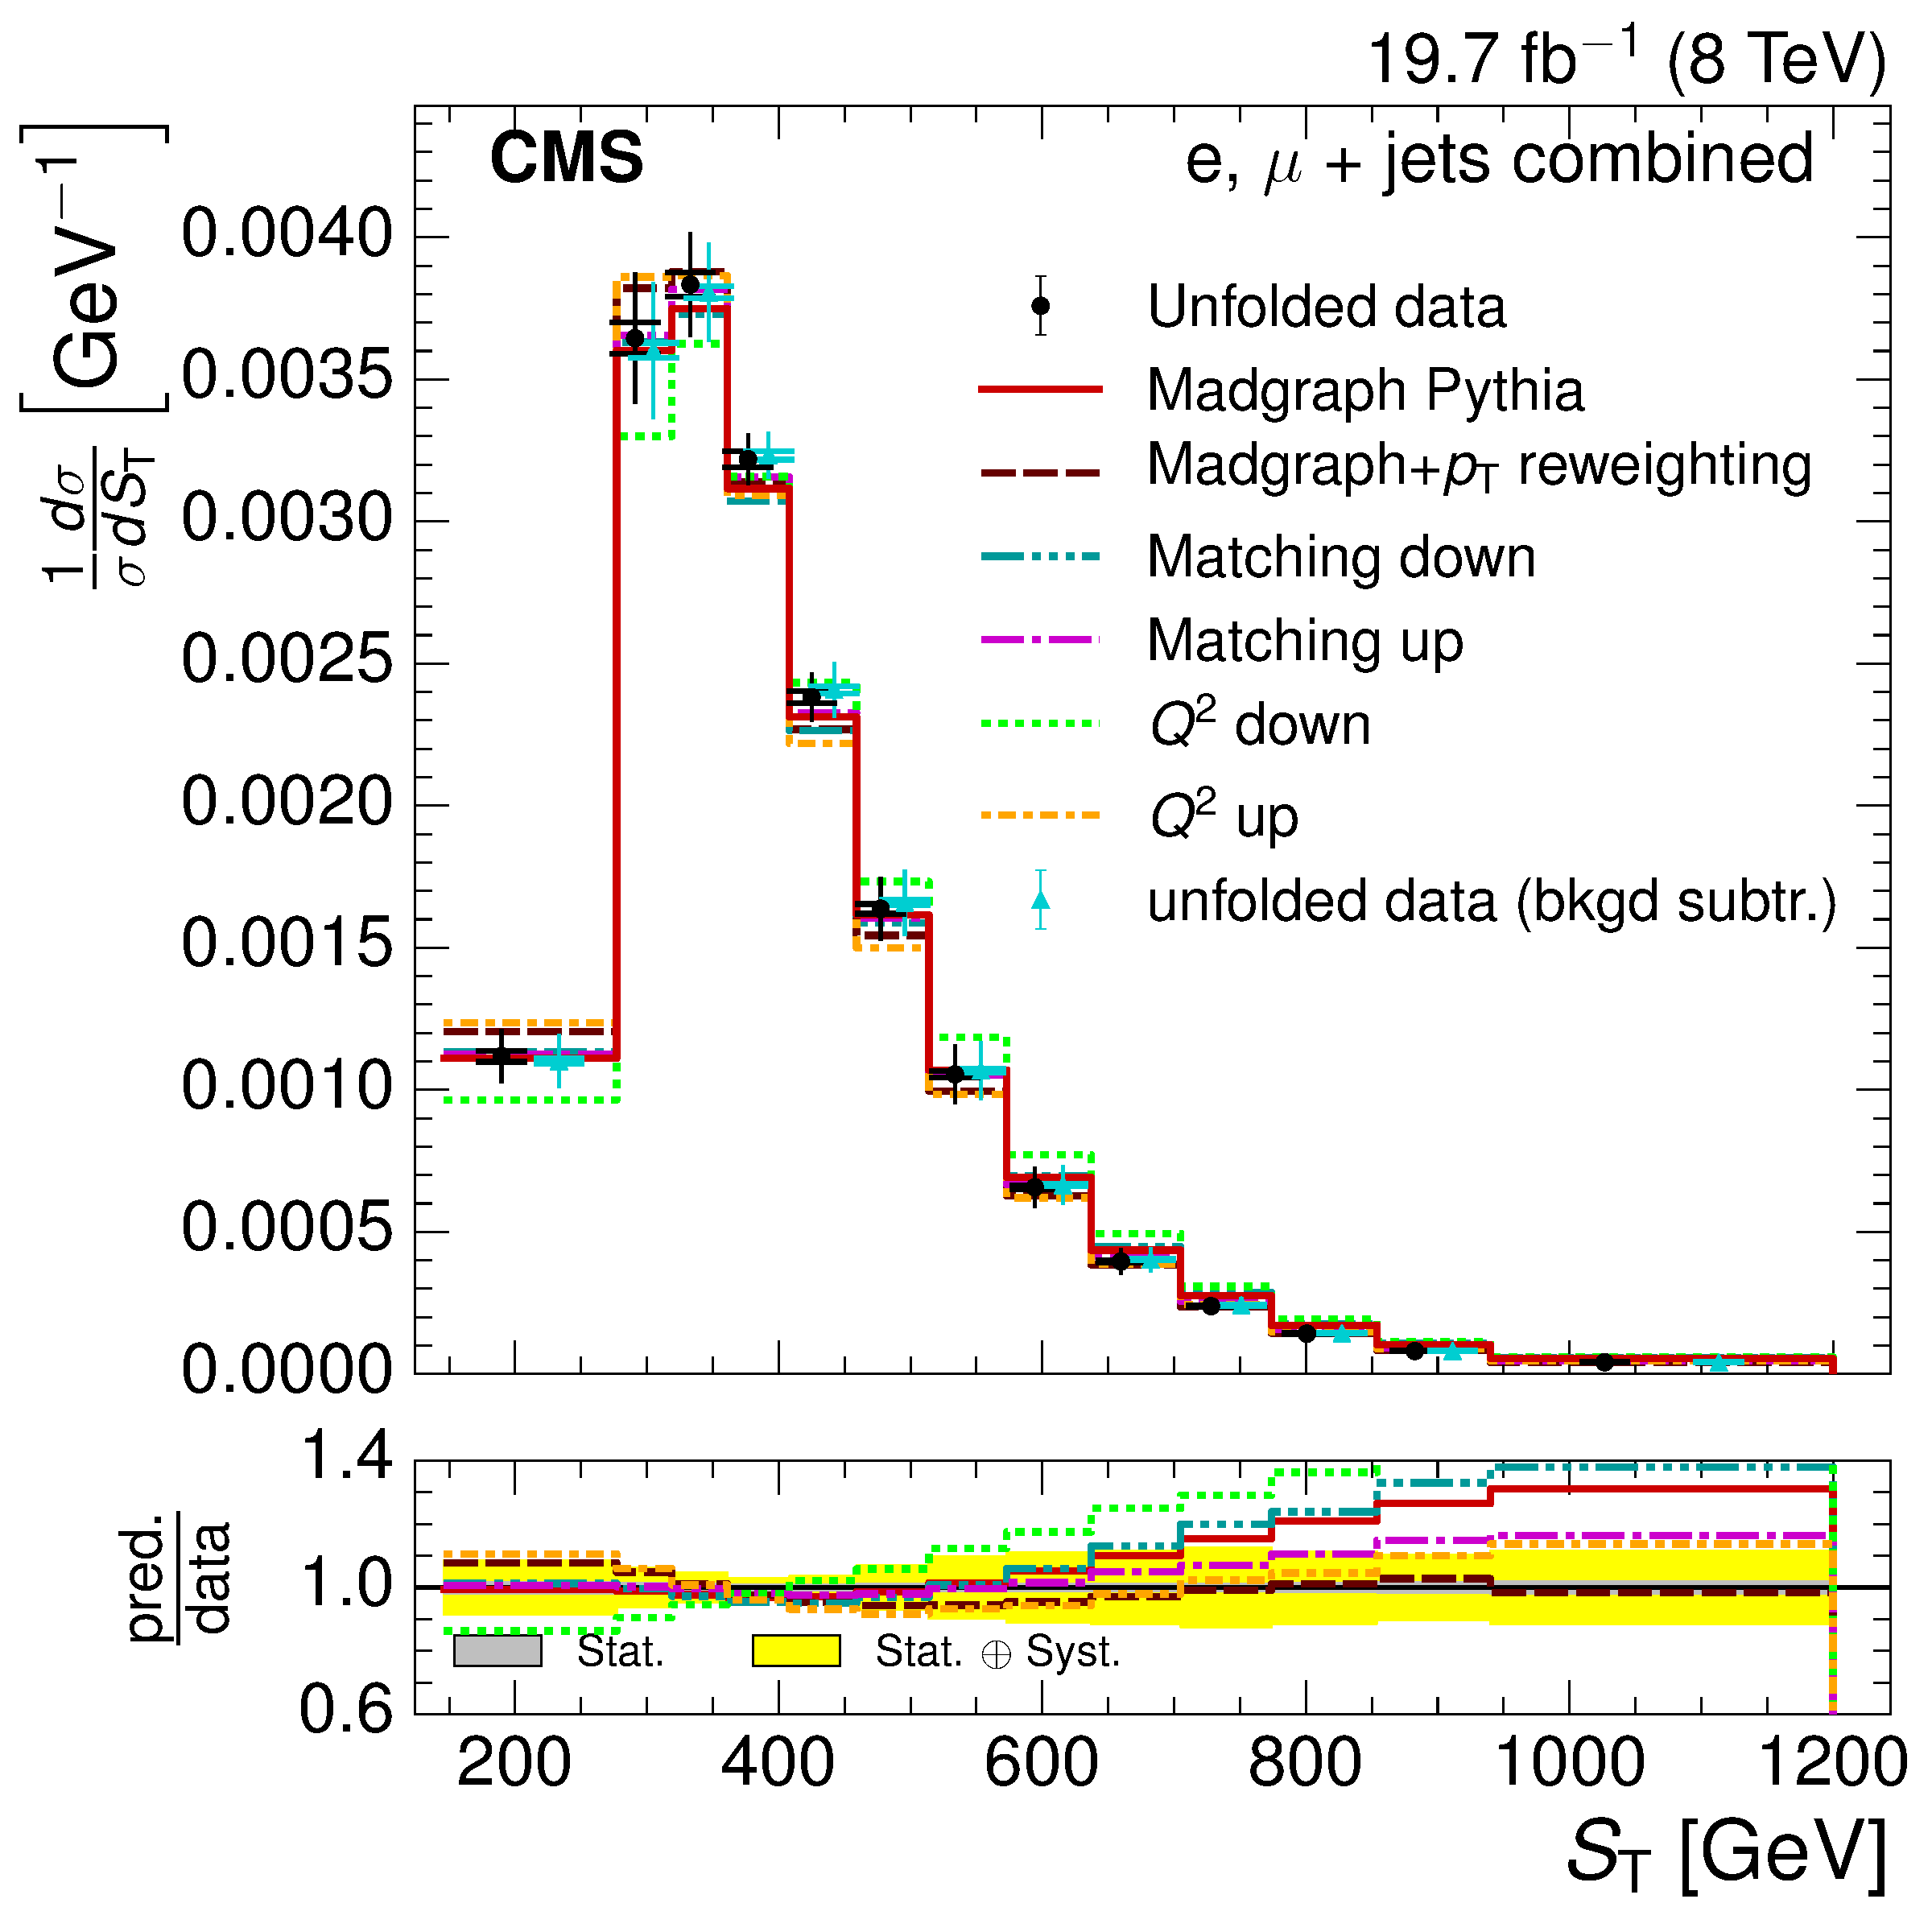
\includegraphics[width=0.32\textwidth]{Chapters/07_08_09_Analysis/Images/results/fit/8TeV/ST/central/normalised_xsection_combined_systematics_shifts_with_bkgd_subtraction_results.pdf}\\
     \caption[Comparison of the measured normalised differential cross section, with background
     subtraction results, with respect to \met, \HT, \st, \wpt and \mt to different Monte Carlo generators and
     predictions at $\roots=8\TeV$.]{Comparison of the measured normalised differential cross section,
     including from the background subtraction method, with respect to \met, \HT and \st, to
     different Monte Carlo generators: \MADGRAPH, \POWHEGHERWIG, \POWHEGPYTHIA and \MADGRAPH corrected for
     top \pt mismodelling (left) and to different Monte Carlo predictions matching threshold up/down and
     factorisation scale up/down (right) in the combined electron+jets and muon+jets channel at
     $\roots=8\TeV$. The lower plots show the ratio of the predictions to the data.}
     \label{fig:result_with_background_subtraction_MET_HT_ST_8TeV_combined}
\end{figure}

\begin{figure}[hbtp]
    \centering
     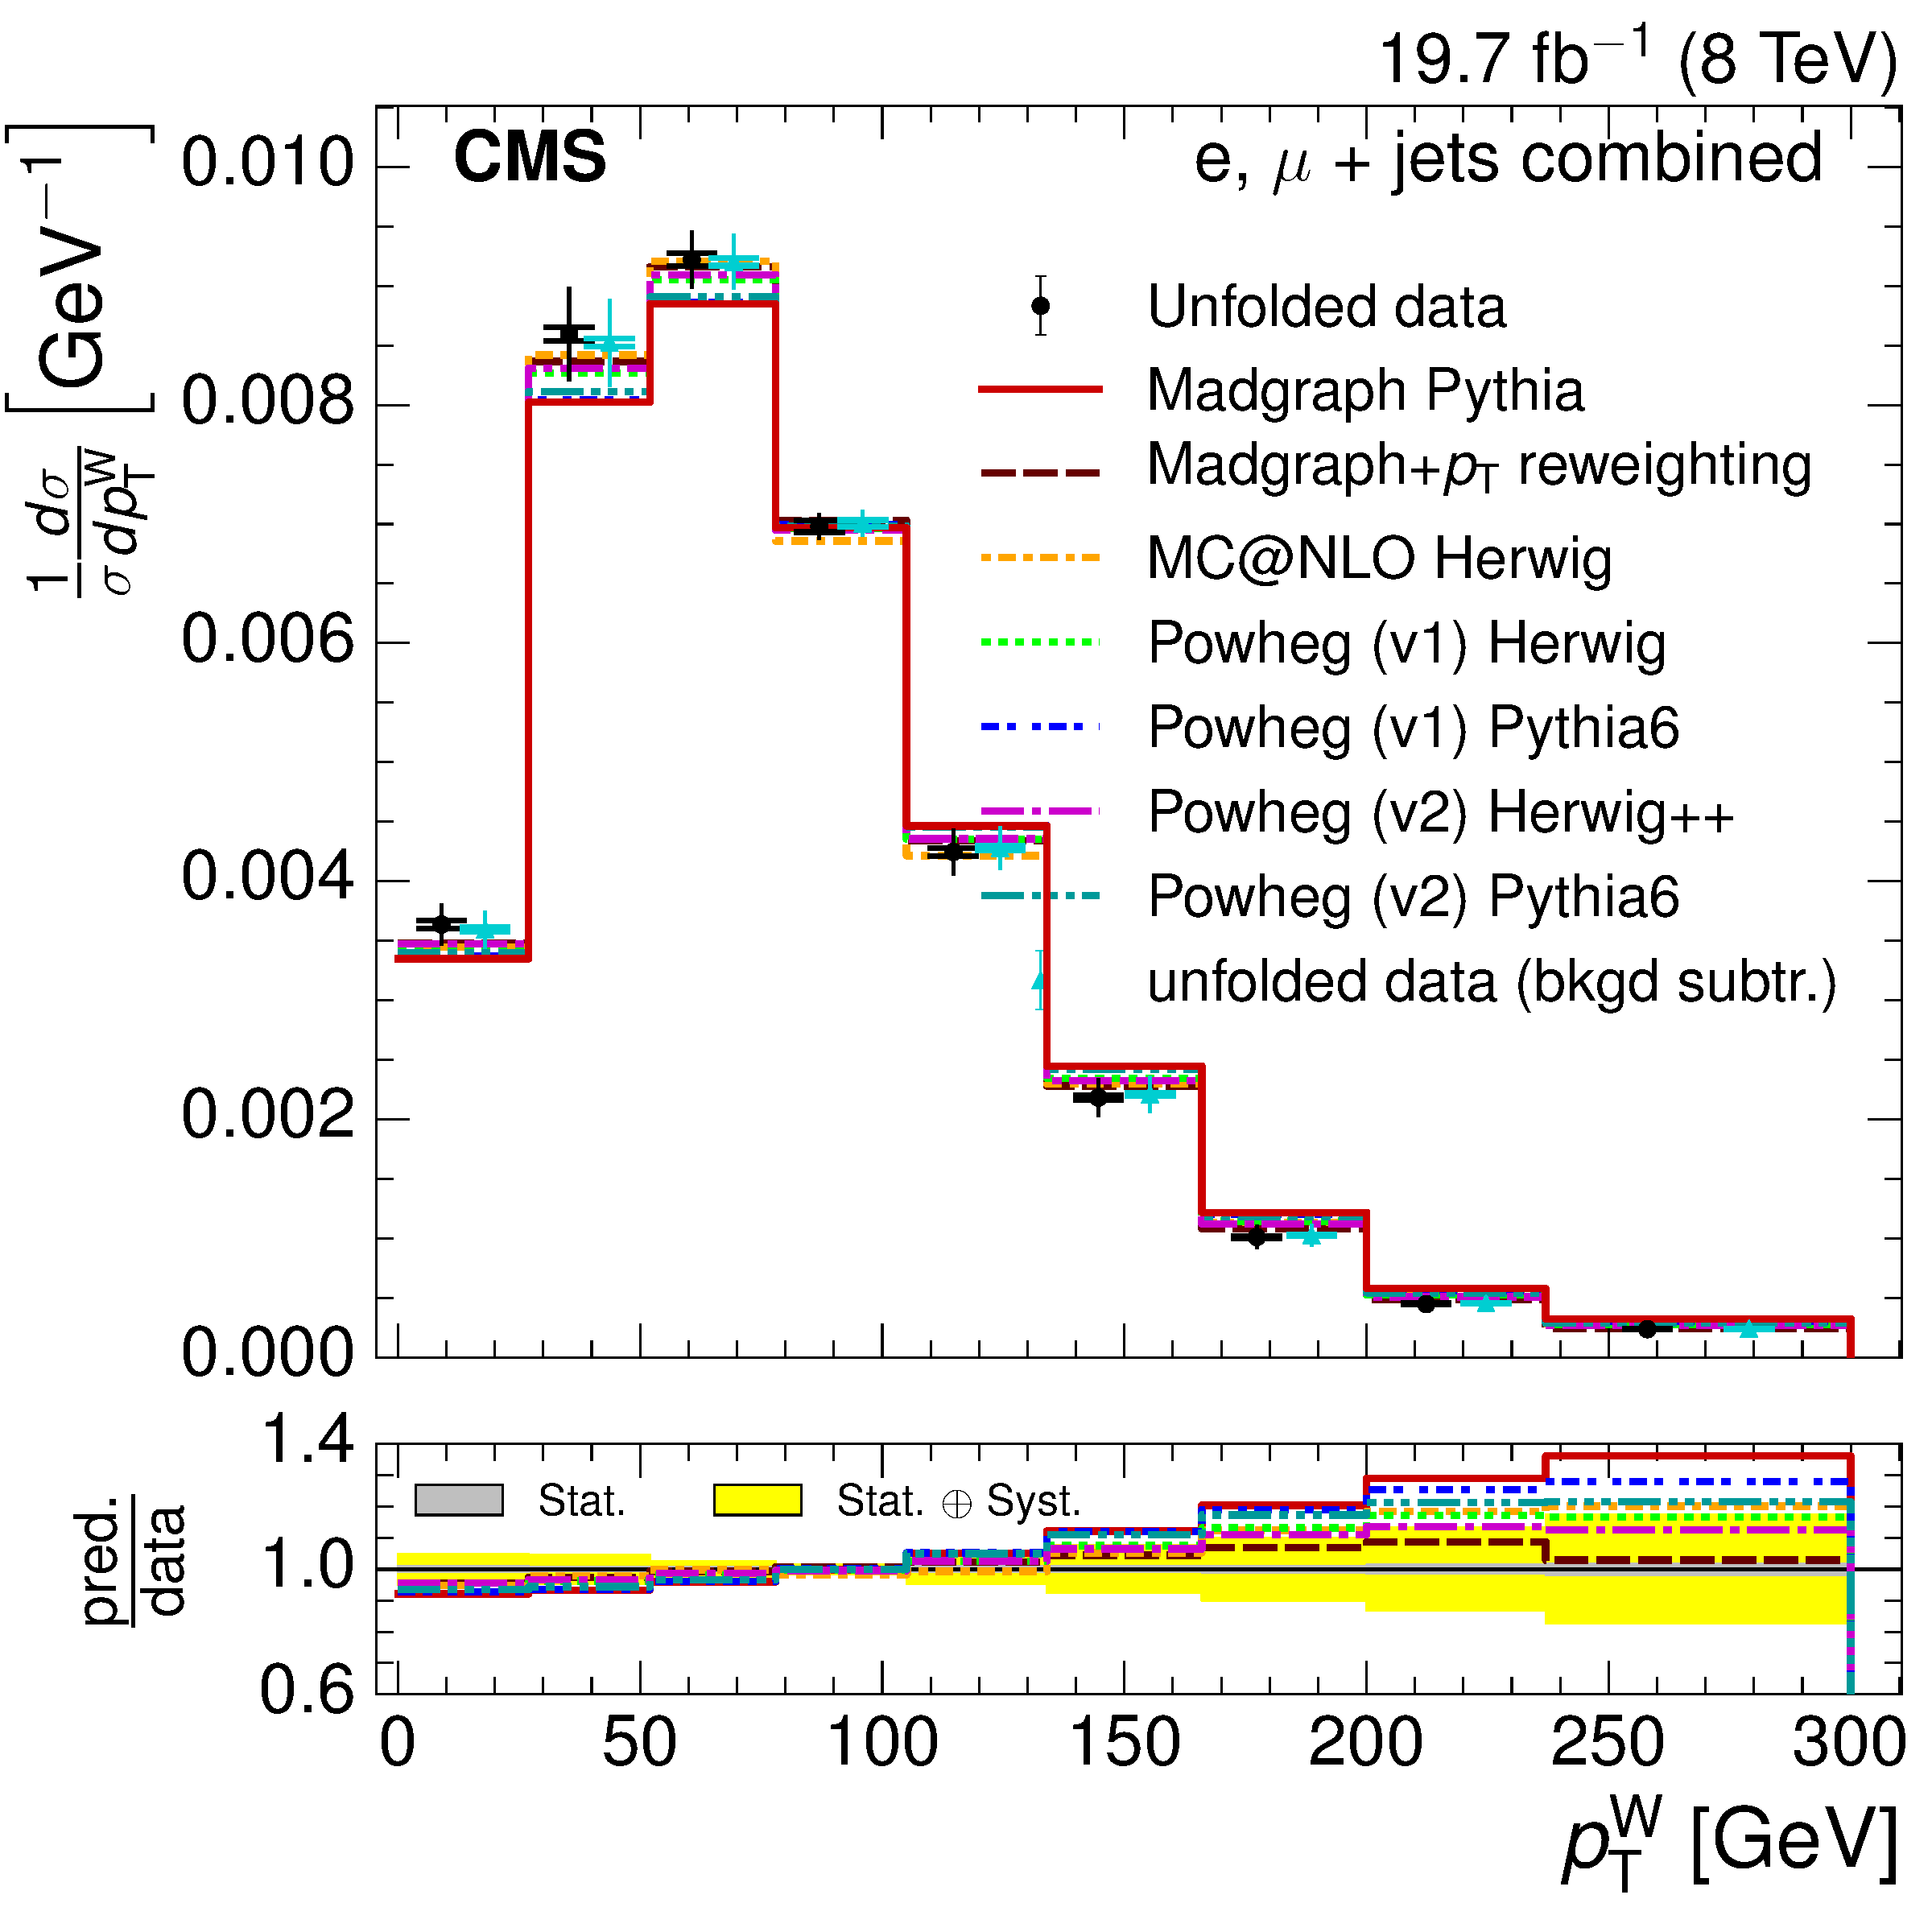
\includegraphics[width=0.32\textwidth]{Chapters/07_08_09_Analysis/Images/results/fit/8TeV/WPT/central/normalised_xsection_combined_different_generators_with_bkgd_subtraction_results.pdf}\hfill
     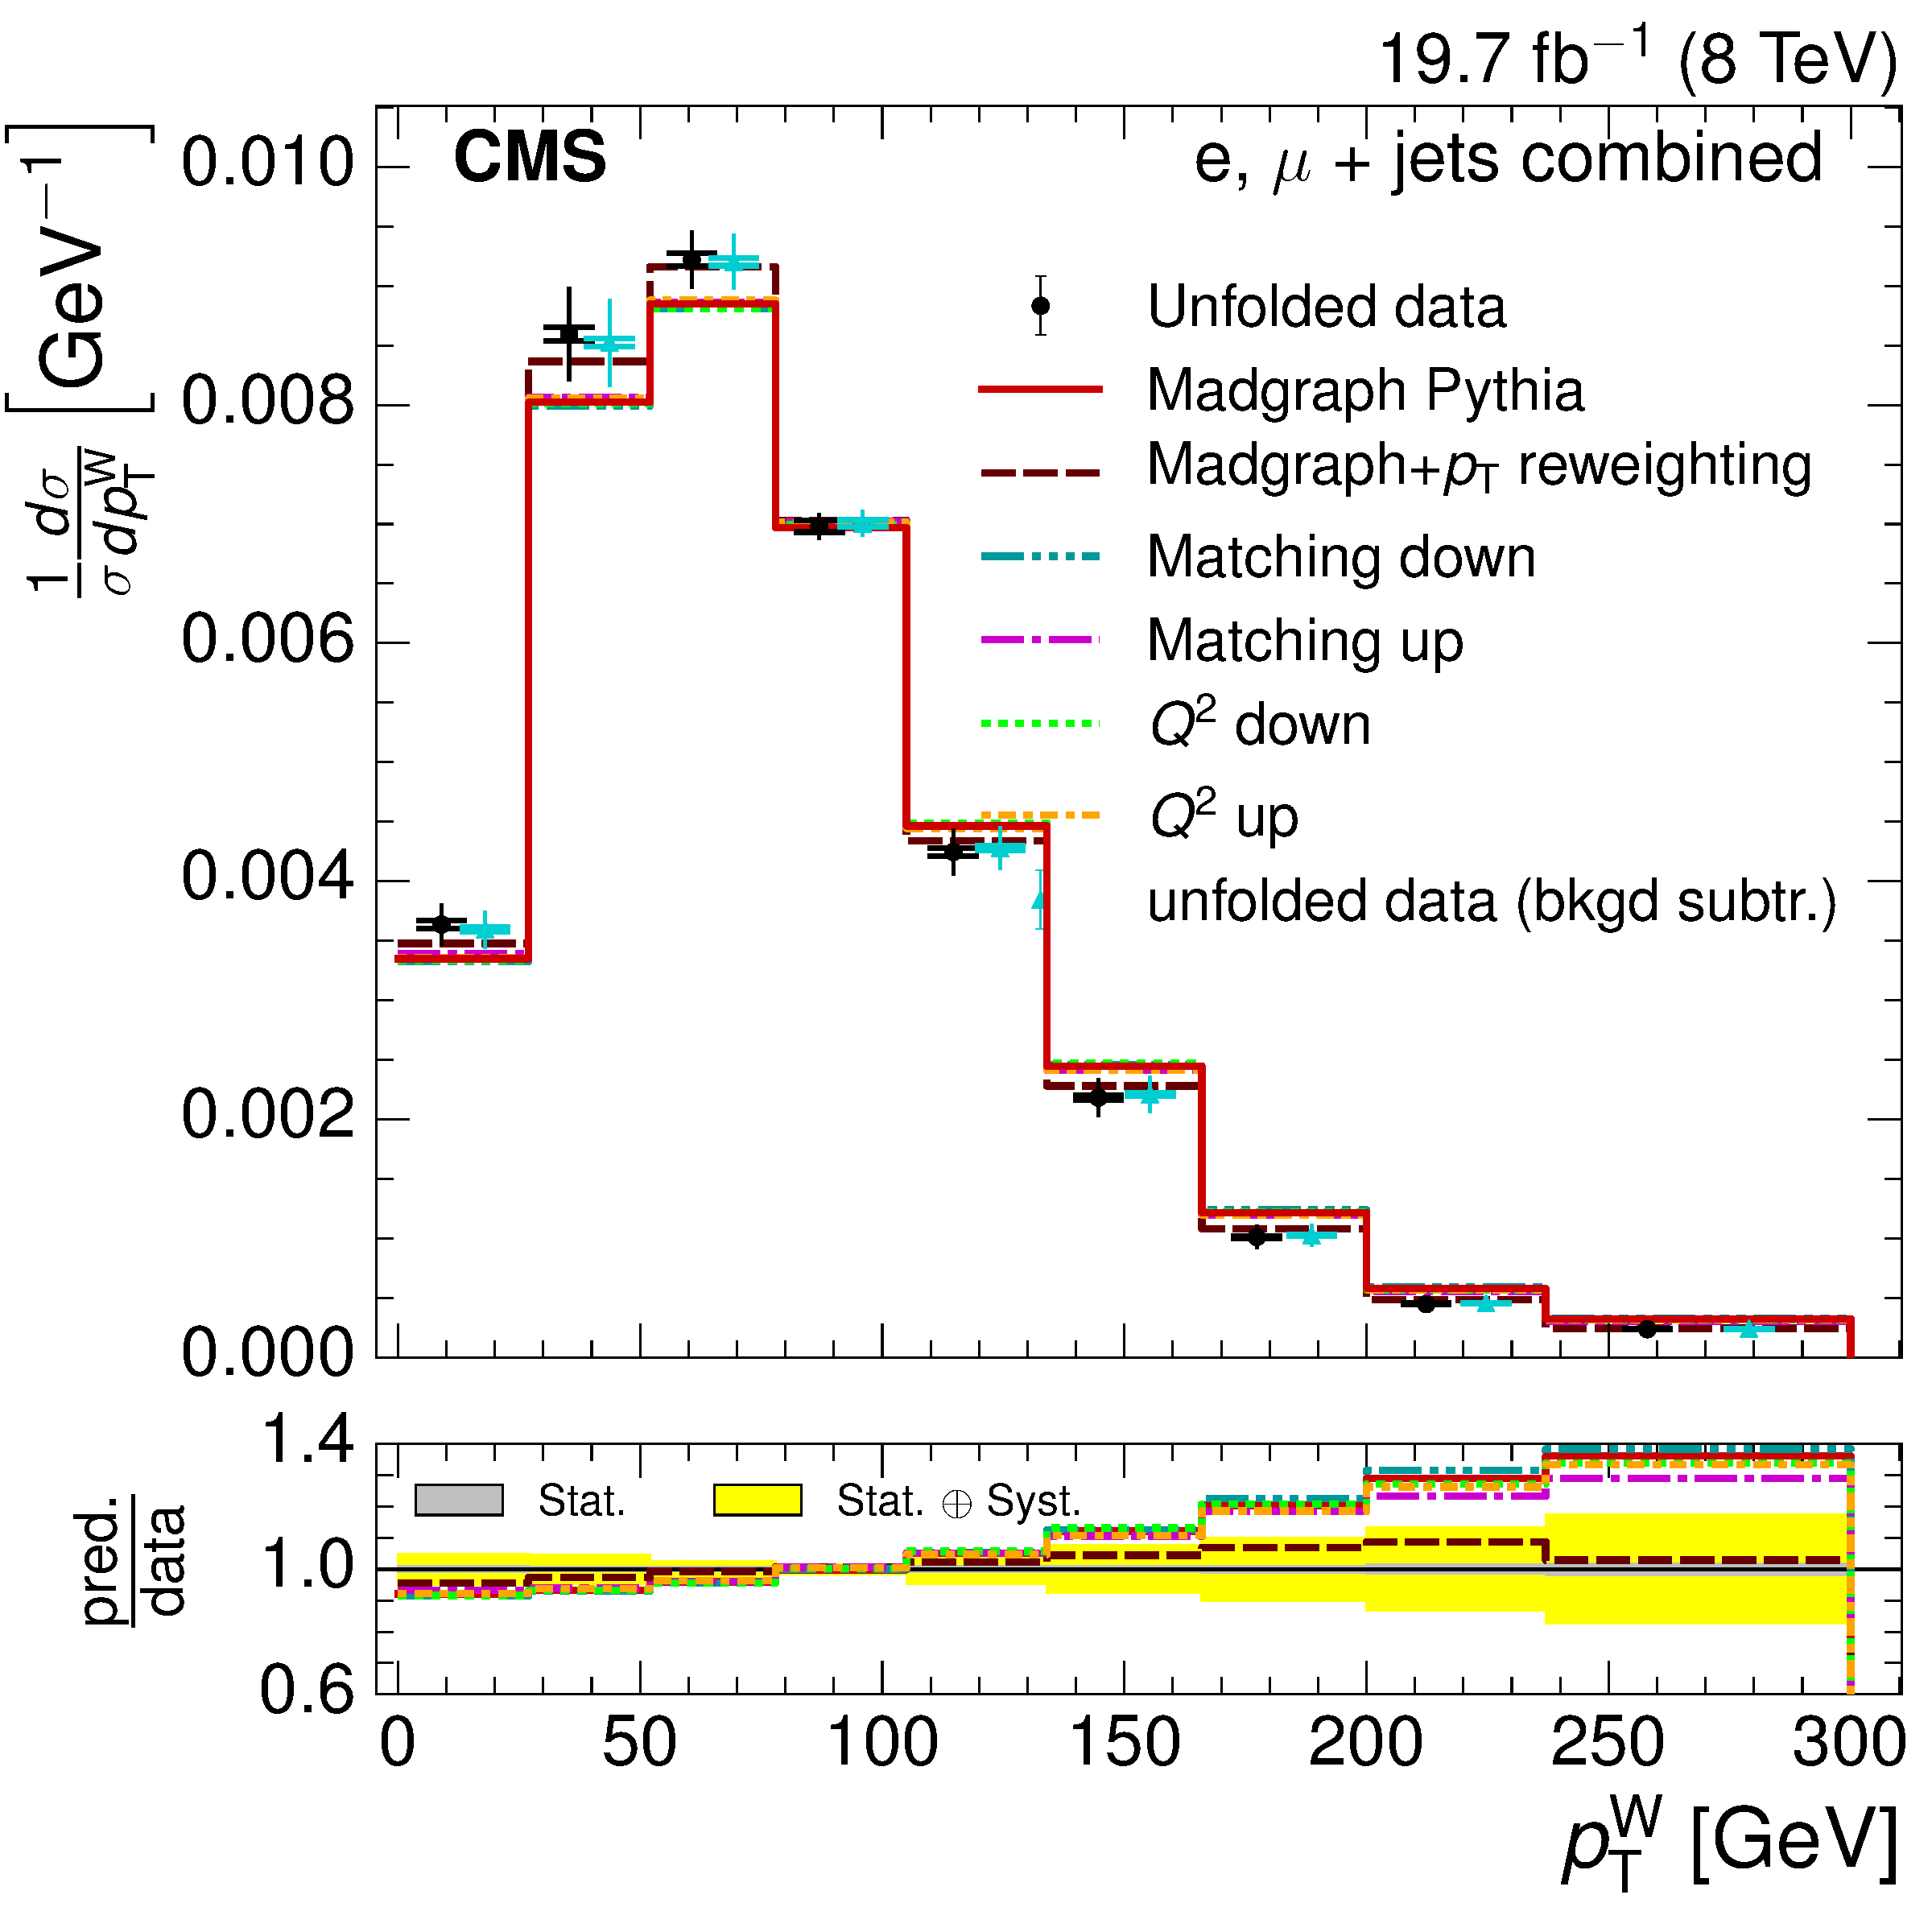
\includegraphics[width=0.32\textwidth]{Chapters/07_08_09_Analysis/Images/results/fit/8TeV/WPT/central/normalised_xsection_combined_systematics_shifts_with_bkgd_subtraction_results.pdf}\\
     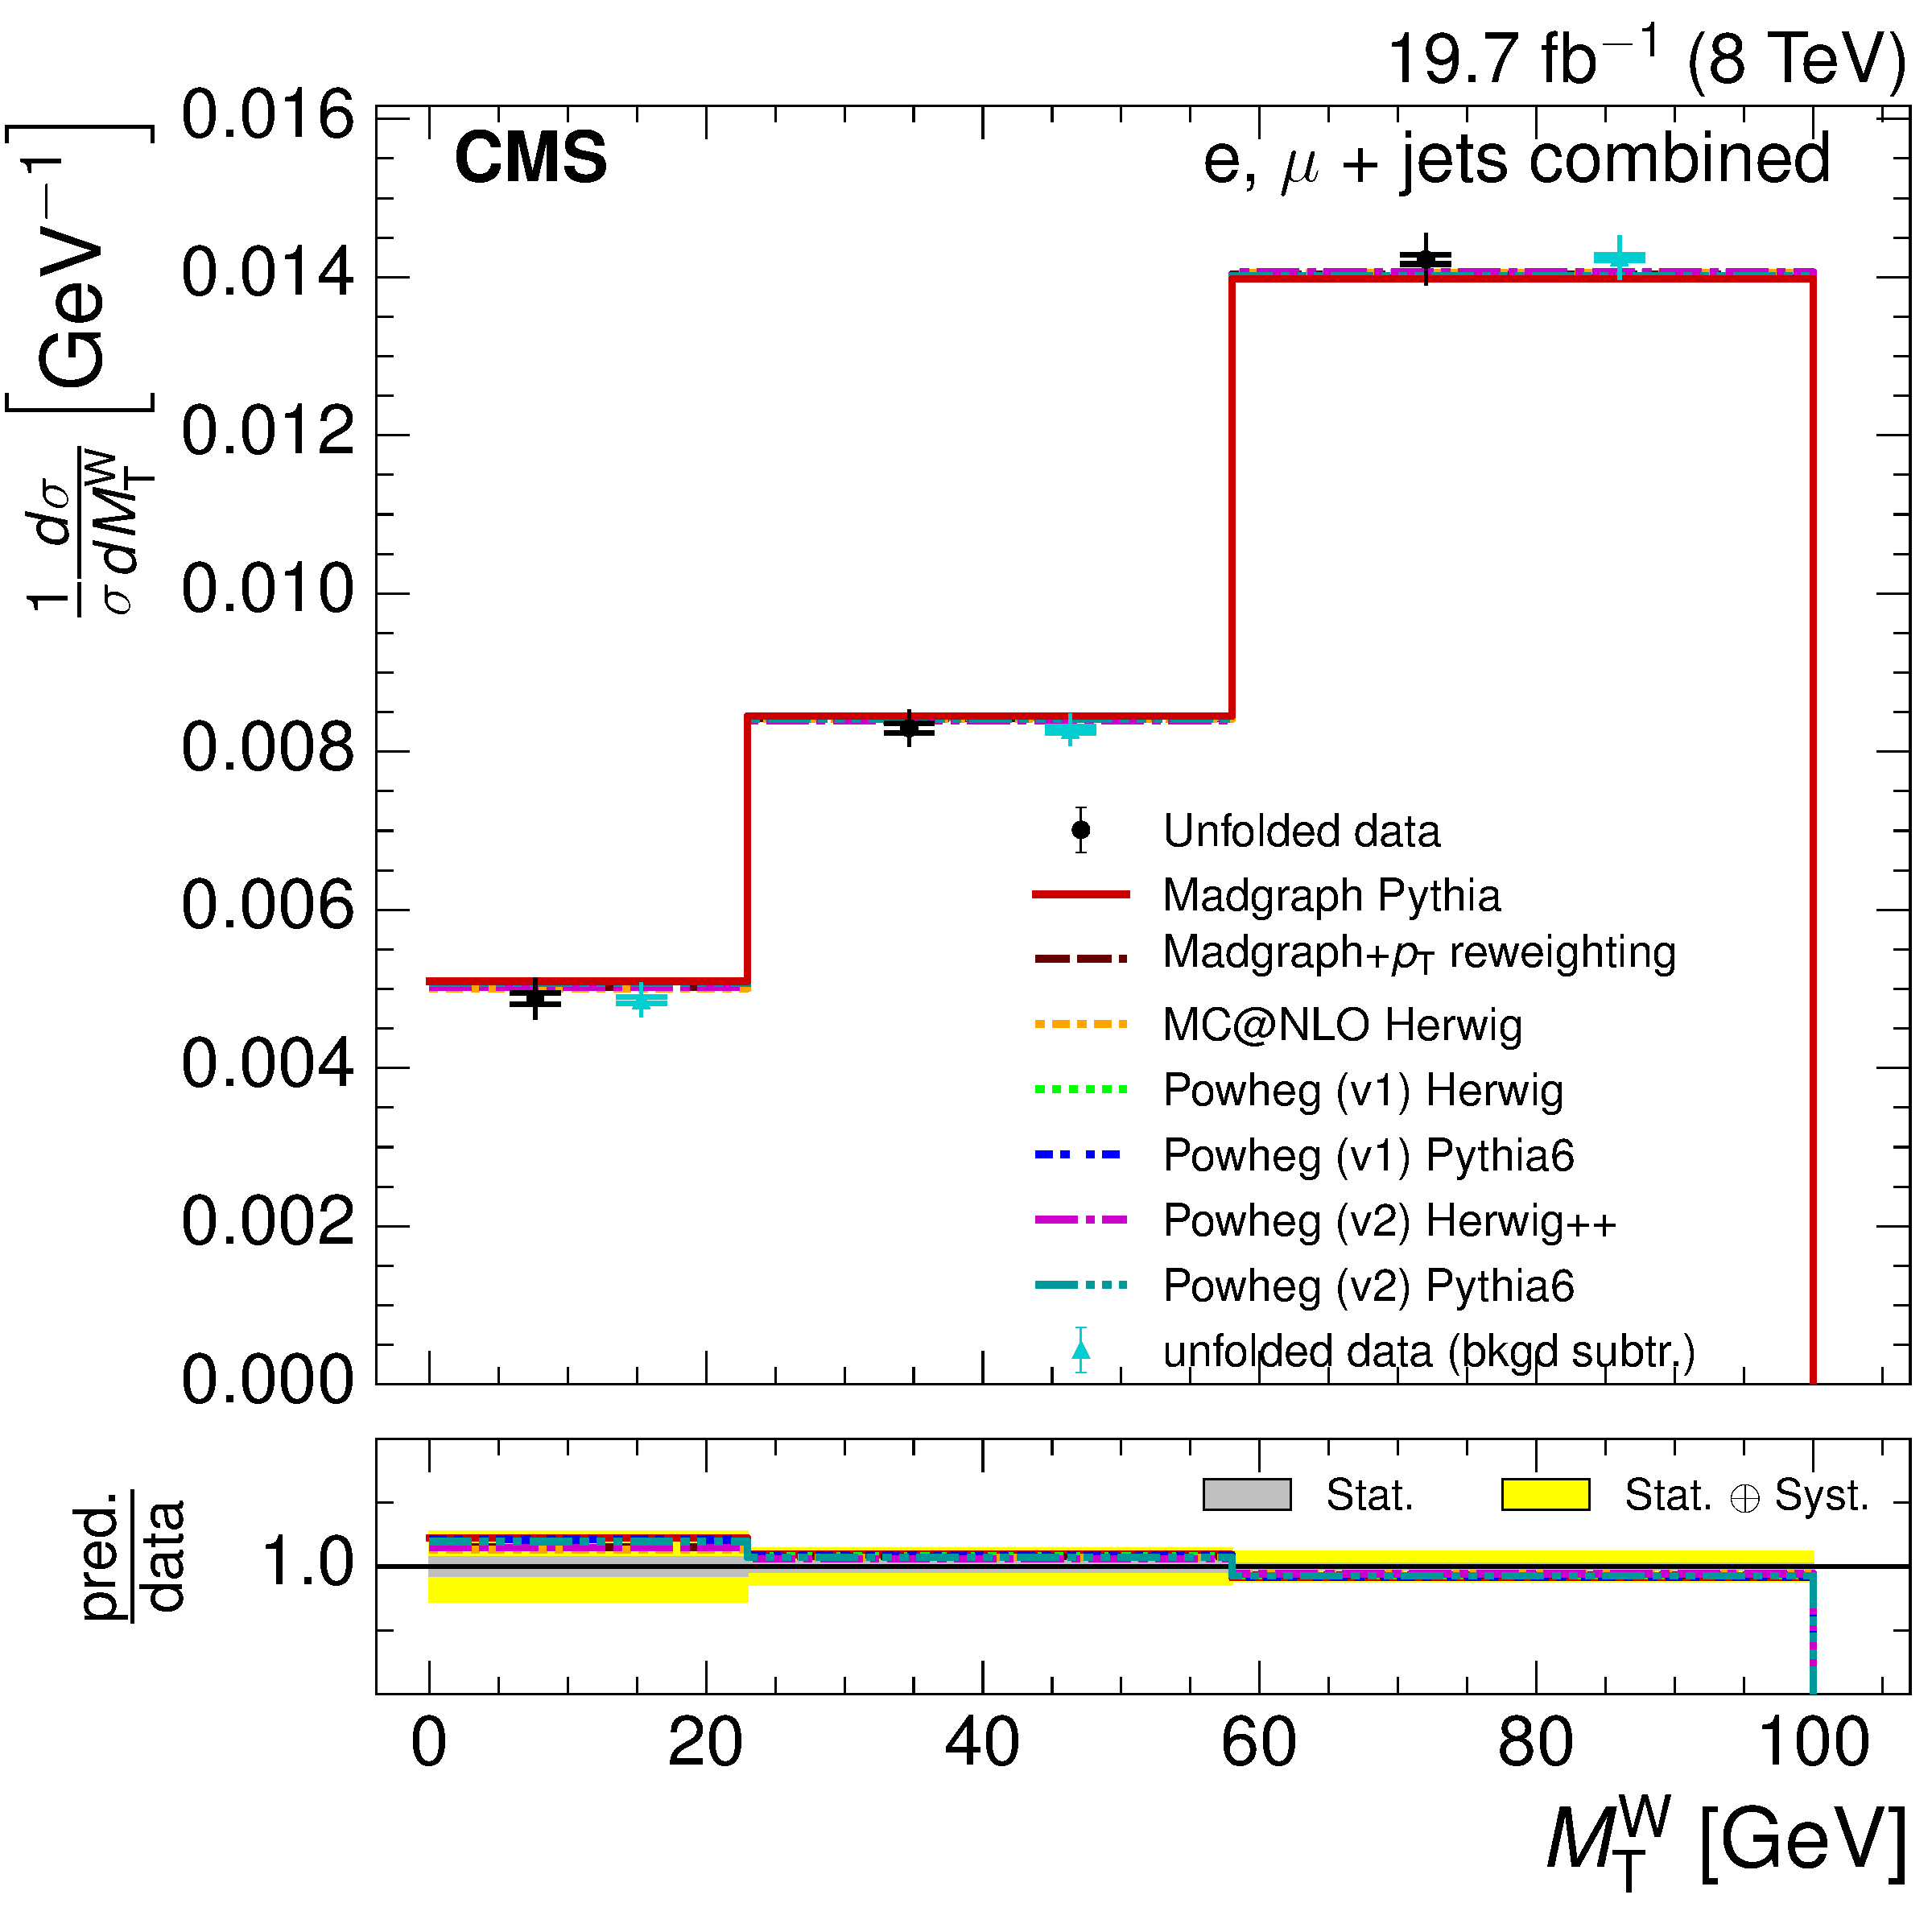
\includegraphics[width=0.32\textwidth]{Chapters/07_08_09_Analysis/Images/results/fit/8TeV/MT/central/normalised_xsection_combined_different_generators_with_bkgd_subtraction_results.pdf}\hfill
     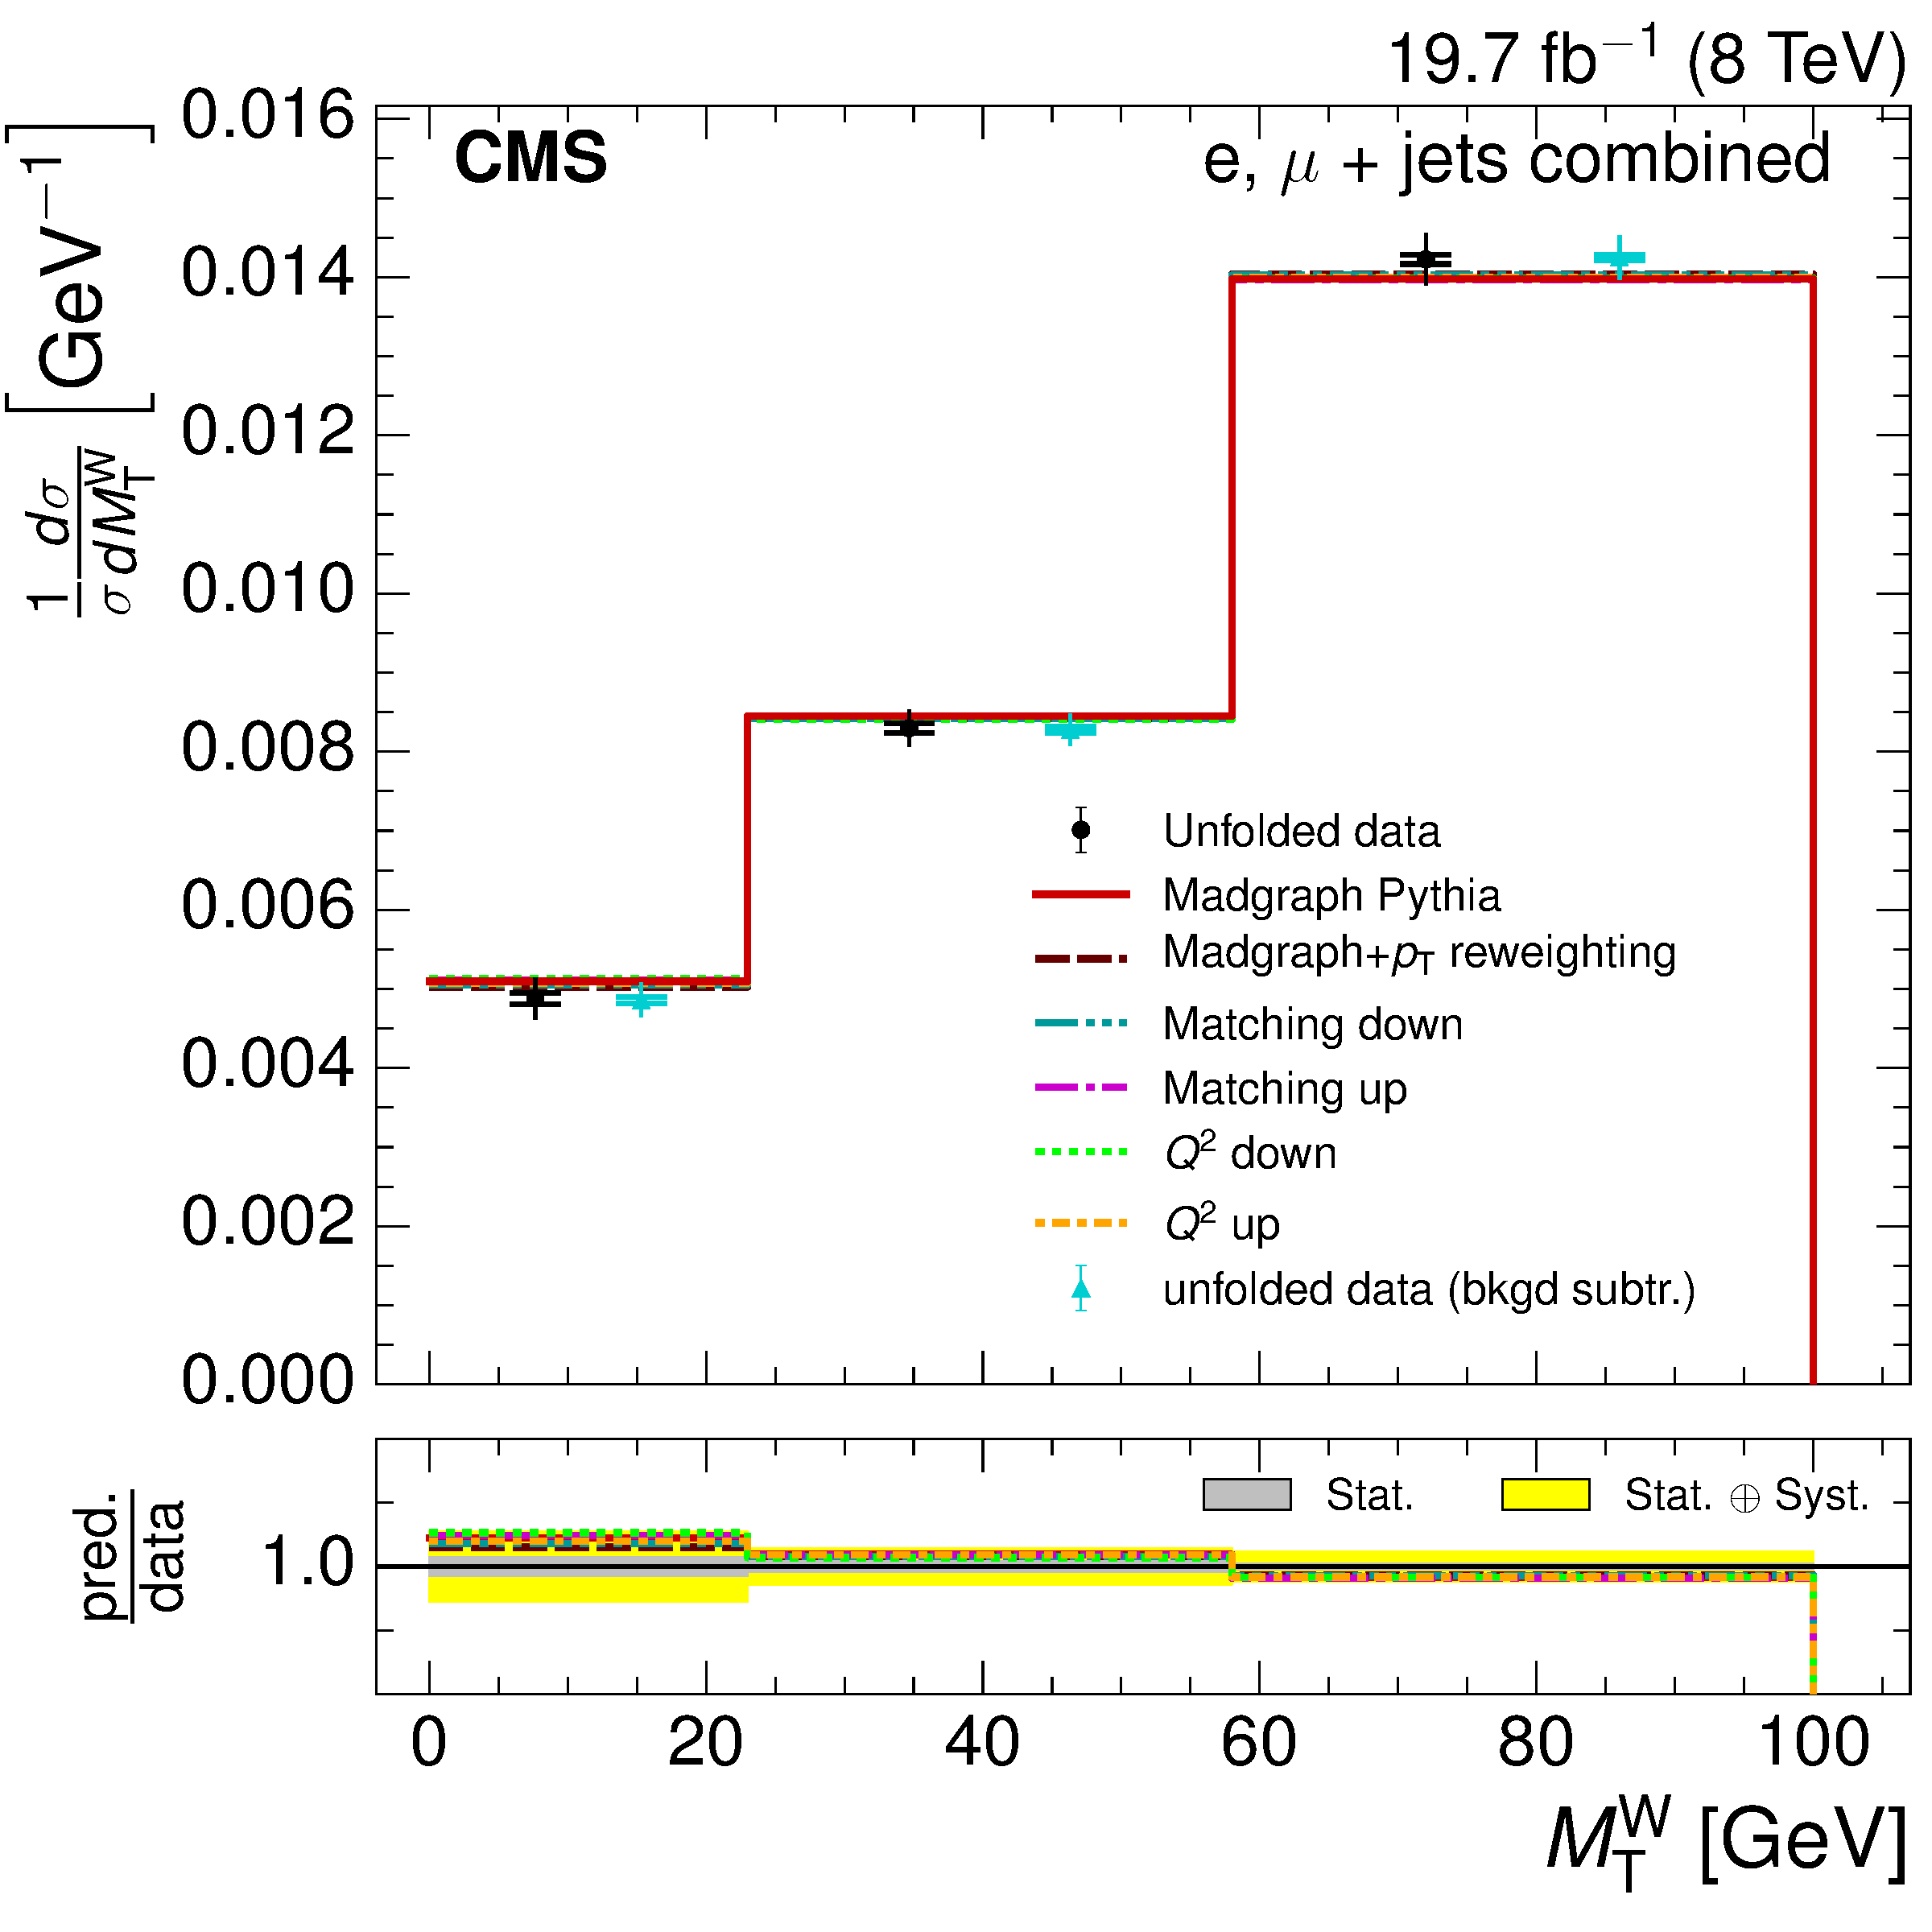
\includegraphics[width=0.32\textwidth]{Chapters/07_08_09_Analysis/Images/results/fit/8TeV/MT/central/normalised_xsection_combined_systematics_shifts_with_bkgd_subtraction_results.pdf}\\
     \caption[Comparison of the measured normalised differential cross section, with background
     subtraction results, with respect to \met, \HT, \st, \wpt and \mt to different Monte Carlo generators and
     predictions at $\roots=8\TeV$.]{Comparison of the measured normalised differential cross section,
     including from the background subtraction method, with respect to \wpt and \mt, to
     different Monte Carlo generators: \MADGRAPH, \POWHEGHERWIG, \POWHEGPYTHIA and \MADGRAPH corrected for
     top \pt mismodelling (left) and to different Monte Carlo predictions matching threshold up/down and
     factorisation scale up/down (right) in the combined electron+jets and muon+jets channel at
     $\roots=8\TeV$. The lower plots show the ratio of the predictions to the data.}
     \label{fig:result_with_background_subtraction_WPT_MT_8TeV_combined}
\end{figure}